% Use only LaTeX2e, calling the article.cls class and 12-point type.

\documentclass[12pt]{article}

% Users of the {thebibliography} environment or BibTeX should use the
% scicite.sty package, downloadable from *Science* at
% http://www.sciencemag.org/authors/preparing-manuscripts-using-latex 
% This package should properly format in-text
% reference calls and reference-list numbers.

\usepackage{scicite}

\usepackage{times}

\usepackage{graphicx,float}

%setup for commenting during editing
\usepackage{xcolor}
\newcommand{\tom}[2]{{\color{red}{#1}}\footnote{\textit{\color{red}{#2}}}}
\newcommand{\josh}[2]{{\color{blue}{#1}}\footnote{\textit{\color{blue}{#2}}}}

% for adjusting the sizes of tables
\usepackage{adjustbox}
% for setting up equations
\usepackage{amsmath}

% The preamble here sets up a lot of new/revised commands and
% environments.  It's annoying, but please do *not* try to strip these
% out into a separate .sty file (which could lead to the loss of some
% information when we convert the file to other formats).  Instead, keep
% them in the preamble of your main LaTeX source file.


% The following parameters seem to provide a reasonable page setup.

\topmargin 0.0cm
\oddsidemargin 0.2cm
\textwidth 16cm 
\textheight 21cm
\footskip 1.0cm


%The next command sets up an environment for the abstract to your paper.

\newenvironment{sciabstract}{%
\begin{quote} \bf}
{\end{quote}}



% Include your paper's title here

\title{Microbial symbionts buffer hosts from the consequences of environmental stochasticity} 


% Place the author information here.  Please hand-code the contact
% information and notecalls; do *not* use \footnote commands.  Let the
% author contact information appear immediately below the author names
% as shown.  We would also prefer that you don't change the type-size
% settings shown here.

\author
{Joshua C. Fowler,$^{1\ast}$ Shaun Ziegler,$^{2}$ Kenneth D. Whitney,$^{2}$\\
	 Jennifer A. Rudgers,$^{2}$ Tom E. X. Miller $^{1}$\\
\\
\normalsize{$^{1}$Rice University, Department of BioSciences, Houston, TX, 77005}\\
\normalsize{$^{2}$University of New Mexico, Department of Biology, Albuquerque, NM, 87131}\\
\\
\normalsize{$^\ast$To whom correspondence should be addressed; E-mail:  jcf3@rice.edu.}
}

% Include the date command, but leave its argument blank.

\date{}



%%%%%%%%%%%%%%%%% END OF PREAMBLE %%%%%%%%%%%%%%%%



\begin{document} 

% Double-space the manuscript.

\baselineskip24pt

% Make the title.

\maketitle 


% Place your abstract within the special {sciabstract} environment.

\begin{sciabstract}
	ABSTRACT: 
Persistence in increasingly variable climates will hinge on species' endurance of environmental stochasticity.
Most organisms host microbiota that can shield against stress, but pinpointing microbial symbionts as buffers against stochasticity requires experiments over long-term, variable climates. 
Stochastic demographic models for seven plant species parameterized with 14 years of symbiont-removal data determined, for the first time, that microbes elevated host fitness by dampening year-to-year fluctuations in demographic performance. 
Hosts with "fast" life histories that lack longevity as an intrinsic buffer experienced the greatest benefits. 
Simulated futures of greater environmental stochasticity amplified the value of variance buffering, which surpassed symbiont benefits to mean host fitness, which preoccupy most prior research.
Results establish microbial symbioses as an important, but cryptic mechanism of resilience to stochastic global change.

\end{sciabstract}


\subsubsection*{One sentence summary suggestions:}
\emph{Epichloë} fungal endophytes buffer their grass hosts from the detrimental effects of environmental variability.

% In setting up this template for *Science* papers, we've used both
% the \section* command and the \paragraph* command for topical
% divisions.  Which you use will of course depend on the type of paper
% you're writing.  Review Articles tend to have displayed headings, for
% which \section* is more appropriate; Research Articles, when they have
% formal topical divisions at all, tend to signal them with bold text
% that runs into the paragraph, for which \paragraph* is the right
% choice.  Either way, use the asterisk (*) modifier, as shown, to
% suppress numbering.

\section*{Main Text}

Global climate change involves increases in environmental variability, including changes to precipitation patterns and the frequency of extreme weather events \cite{IPCC2012managing,seneviratne2012changes,stocker2013technical};
yet, the consequences of increased variability are less well understood than those of changing climate means, such as long-term warming or drying. 
Incorporating environmental variability into forecasts of population dynamics can improve predictions of the future.
Classic theory predicts that long-term population growth rates (equivalently, population mean fitness) will decline under increased environmental variability because the costs of bad years outweigh the benefits of good years -- a consequence of nonlinear averaging \cite{lewontin_population_1969,tuljapurkar_population_1982}.
For example, in unstructured populations, the long-term stochastic growth rate in fluctuating environments ($\lambda_s$) will always be lower than the growth rate averaged across environments ($\overline{\lambda}$) by an amount proportional to the environmental variance ($\sigma^2$): 
\begin{equation}
	 log(\lambda_s)  \approx log(\overline{\lambda}) - \frac{\sigma^2}{2\overline{\lambda}^2}
\end{equation}

\noindent Populations structured by size or stage similarly experience costs of variability \cite{cohen1979comparative,tuljapurkar2013population}.
There are accordingly two pathways to increase population viability in a variable environment: increase the mean growth rate and/or dampen temporal fluctuation in growth rates, also called ``variance buffering''.

Both the characteristics of species and the properties of their environment can buffer demographic fluctuations, including life history traits such as longevity \cite{pfister1998patterns, morris2008longevity}, correlations among vital rates \cite{compagnoni2016effect}, transient shifts in population structure \cite{ellis2013role}, the magnitude of environmental variability \cite{rodriguez2021limits}, or the degree of environmental autocorrelation \cite{tuljapurkar1980population,fieberg2001stochastic}. 
These characteristics and properties determine the risks of extinction faced by populations \cite{menges2000applications} and underlie conservation management strategies promoting ecosystem resilience \cite{kuparinen2016fishing}. 
Yet little is known about how biotic interactions influence demographic variability \cite{hilde_demographic_2020}. 

Most multicellular organisms host symbiotic microbes that affect growth and performance \cite{rodriguez2009fungal,mcfall2013animals}, and many of these are transmitted via reproduction from maternal hosts to offspring \cite{funkhouser2013mom}.
This process of vertical transmission links the fitness of hosts and symbionts in a feedback loop that selects for mutual benefits \cite{ewald1987transmission,fine1975vectors}.
Many vertically transmitted microbes are mutualistic and protect hosts from environmental stresses including drought, extreme temperatures, or natural enemies \cite{russell2006costs,brownlie2009symbiont,kivlin2013fungal,corbin2017heritable,hoadley2019host}. 
However, these protective mutualisms are context-dependent: the magnitude of benefits depends on environmental or biotic conditions \cite{chamberlain2014context} and thus will vary temporally in a stochastic environment \cite{jordano1994spatial,billick2003relative}.
We hypothesized that context-dependent benefits from symbionts may buffer hosts against variability through strong benefits during harsh periods, and neutral or even costly outcomes during benign periods, reducing the impacts of host exposure to extremes and dampening inter-annual variance relative to non-symbiotic hosts.
Variance buffering is a previously unexplored mechanism by which symbionts may benefit their hosts, in addition to elevating average fitness,. Variance buffering is likely to increase in importance in a more variable future \cite{rudgers2020climate}.

We tested the hypothesis that context-dependent benefits of symbiosis buffer hosts from the fitness costs of environmental variability using data from long-term, symbiont-removal experiments. 
We  (i) quantified the effects of symbiosis on the mean and variance of host vital rates (survival, growth and reproduction), (ii) evaluated the relative contribution of mean and variance effects to long-term population growth rates ($\lambda_s$), (iii) investigated the relationship between host life history traits and the magnitude of symbiont-mediated variance buffering, and (iv) projected the consequences of variance buffering to population growth with simulations of increased variability.

Our experiment began in 2007 in south-central Indiana, USA with seven grass species that host \emph{Epichlo\"{e}} fungal endophytes. The experiment consisted of annually censused populations founded with either naturally symbiotic plants (S+) or those which have had their symbionts experimentally removed  via a heat treatment (S-) (See Materials and Methods for a full list of species and experimental methods).
\emph{Epichlo\"{e}} fungi are specialized symbionts growing intercellularly in the aboveground tissue of  $\sim30$\% of cool-season ($C_{3}$) grass species \cite{leuchtmann1992systematics}.
The fungi are primarily transmitted vertically from maternal plants through seeds \cite{cheplick2009ecology,rudgers2009fungus}.
They produce a variety of alkaloids that can protect host plants from herbivory \cite{brem2001epichloe} and drought stress \cite{cheplick2004recovery,kannadan2008endophyte,decunta2021systematic}.

The unique data from this long-term experiment are distinctly suitable for detecting fitness benefits of microbial symbiosis that arise through variance buffering. 
We collected annual demographic data on the vital rates (survival, growth, and reproduction) of all plants within replicated S+ and S- plots, which on average had 13.3 individuals/$m^2$ over the course of the experiment. 
Each census year was a sample of interannual climatic variation (n = 14 years).
We fit hierarchical Bayesian generalized linear mixed models to the vital rate data using RStan \cite{rstan2022}, which allowed us to isolate endophyte effects on vital rate means and variances, borrow strength across species for some variance components, and propagate uncertainty from the individual-level vital rate to our population model \cite{elderd2016quantifying}. 
We then parameterized stochastic matrix population models for each of the seven grass host species from the vital rate regressions to quantify endophyte effects on stochastic population growth rates ($\lambda_s$) and decompose the overall effect of the symbiosis into contributions through mean vital rates, variance in vital rates, and their interaction (Supplemental Material describes the statistical methods in full).

Across seven host species, eight vital rates, 14 years, and 16,789 individual plants, our analysis provides the first empirical support for the hypothesis of symbiont mediated variance buffering. Endophytes reduced inter-annual variance for 66\% ($37$/$56$) of host species-vital rate combinations (average Cohen's D for effects on vital rate standard deviation: $-0.15$) (Fig 1A). 
Endophytes also increased the mean for the majority of host species and vital rates ($36$/$56$) (average Cohen's D for effects on vital rate mean: $0.15$), and benefits were particularly strong for host survival, plant growth and germination (Fig. 1A).
Endophytes also reduced inter-annual variance for the majority of host species and vital rates 
The relative magnitude of symbiont effects on means versus variances differed among grass species and their vital rates.
For example, endophytes modestly increased mean adult survival (Fig. 1C) and reduced variance in survival (Fig. 1D) for \emph{Festuca subverticillata}, while for \emph{Poa alsodes}, variance buffering was more apparent in seedling growth and inflorescence production (Fig 1E). 
Interestingly, certain vital rates showed costs of endophyte symbiosis. 
Symbiotic individuals of \emph{A. perennans} grew larger than those without endophytes (Fig. 1B), yet endophytes also reduced this species' mean germination rates (Fig. 1A). 
Similarly, endophyte symbiosis increased variance in seedling growth for \emph{Elymus villosus} and \emph{Festuca subvertcillata} (Fig. 1A).
 
 The coefficient of variation of $\lambda$, reflecting inter-annual variability in population fitness, was $40$\% lower in endophyte-symbiotic populations than endophyte-free populations, (with $>86$\% confidence that the endophyte effect was dampening) (Fig. 2B).
For some host species, the coefficient of variation was reduced by as much as $170$\% (\emph{P. alsodes},\emph{F. subverticillata}), while for others, endophyte effects were substantially smaller ($6$\% - \emph{E. villosus}, $16$\% - \emph{A. perennans}), or even positive ($27$\% increase - \emph{E. virginicus}).
These results derived from stochastic matrix models with plant size (tiller number) as the integer-valued state variable to integrate the diverse effects on vital rates described above into comprehensive measures for the mean and variance of annual fitness ($\lambda$), because not all vital rates contribute equally to population growth.
In addition to the variance effect, on average across host species, endophyte-symbiotic populations had \tom{$9$\%}{would like to discuss} greater mean growth rates, $\overline{\lambda}$, than endophyte-free populations (Fig. 2A). 
Our hierarchical Bayesian analysis, which propagated uncertainty from the underlying data through model predictions, indicated $>92$\% confidence that endophytes increased $\overline{\lambda}$.
When the two mechanisms, via variance or via mean effects, were considered together, none of the host-symbiont pairings were antagonistic (i.e., with endophytes that both decreased mean and increased variance) (Fig. 2C), suggesting that variation the across host species in mean and variance effects may reflect alternative life history strategies that yield similar benefits of endophyte symbiosis.

Long-lived species, those on the slow end of the slow-fast life history continuum, are expected to be less sensitive to environmental variability \cite{murphy1968pattern}, a pattern which has empirical support across plants \cite{compagnoni2021herbaceous} and animals \cite{le2022life,morris2008longevity}.
Therefore, we predicted that host species with slower life histories that produce fewer, large offspring that persist through environmental variability would benefit less from the variance buffering effects of endophytes than species with fast life histories that produce many smaller offspring with low per-capita chance of success) \cite{rees1996evolutionary,moles2004seedling}.
In support of this prediction,  symbiota with trait values representing faster life history strategies experienced greater variance buffering from endophytes (Fig. 3) than those with slow life histories. 
For example, variance buffering was stronger for host species with smaller seeds (Fig. 4E; 74\% probability of positive relationship) and shorter longevity (Fig. 4C; 64\% probability of positive relationship).
Other life history traits similarly had positive but weaker support for the prediction that slower life traits would correlate with stronger variance buffering (Fig. S27).
We calculated demographic life history traits (generation time, longevity, and net reproductive rate) from matrix models for symbiont-free populations using the Rage package \cite{jones2022rcompadre} and we collated other traits from the literature (seed length) and from the experimental plots (99th percentile of maximum observed age). 
We used Bayesian phylogenetic mixed-effects models to assess the relationship between these traits and the variance buffering effect of symbiosis, propagating uncertainty associated with estimated variance buffering effects (Supplemental Methods).
Additionally, in our study, the three host species for which the overall mutualism was weakest (\emph{Elymus villosus}, \emph{Elymus virginicus}, and \emph{Poa sylvestris}) (Fig. 2C) were the only hosts for which we observed stromata, fungal fruiting bodies capable of horizontal (contagious) endophyte transmission (Table S2), in line with theoretical expectations for strict vertical transmission to drive the evolution of mutualisms \cite{fine1975vectors,afkhami2008symbiosis}.
Conclusions about life histories are limited by traits spanning a relatively narrow range of values due to the number of species in our experiment and, their shared evolutionary histories within the Pooidae. 
Our understanding of the role of symbiosis in life history theory would profit from tests for variance buffering across a wide span of taxonomic groups \cite{jeschke2009roles}.

Reduced sensitivity to drought, as has been reported for some \emph{Epichlo\"{e}} symbioses \cite{decunta2021systematic}, is a candidate mechanism that could generate a signature of variance buffering.
Accordingly, analysis of a climate-explicit population model indicated that for five of seven taxa, symbiotic populations were less sensitive to annual or growing season drought (12-month or 3- month drought index; Standardized Precipitation Evaporation Index) \cite{vicente2010multiscalar}) than symbiont-free populations (Fig. S24-S25; Table S3) (Supplemental Methods).
However, we did not find a strong relationship between the magnitude of variance buffering and relative drought sensitivities, suggesting that other climatic factors or other aspects of the abiotic or biotic environment may elicit benefits of endophyte symbiosis, including documented resistance to herbivory for six of the taxa \cite{rudgers2008invasive,crawford2010fungal}
Identifying the potentially complex relationships between vital rates and environmental drivers remains a key challenge for accurate forecasts of the ecological impacts of environmental stochasticity \cite{ehrlen2015predicting}.


Endophytes' contributions to the stochastic growth rate ( $\lambda_s$) from mean effects were four times greater, averaged across species, than contributions from variance buffering (Fig. 4),  suggesting that, under the regime of environmental variability represented by our 14-year study, dampened fluctuation is a far less important element of the benefits of symbiosis than elevated mean fitness of symbiotic plants. 
Overall, the full effect of symbiosis on $\lambda_s$, averaged across host species, provided strong evidence of grass-endophyte mutualism (100\% certainty of a positive total effect on $\lambda_s$) (Fig. 4; see Fig. S21 for individual host species).
Contributions to the total effect on $\lambda_s$ derived from both mean and variance buffering effects, as well as a slightly negative interaction (i.e., the combined influence of mean and variance effects was lower than the sum of their individual effects). To evaluate the relative importance of these pathways of mutualism (via mean benefits or variance buffering), we decomposed  the overall effect of the symbiosis on $\lambda_s$ using stochastic simulations of four versions of population models. 
The models included both mean and variance buffering effects, mean effects alone, variance effects alone, or neither mean nor variance effects. 
We ran each simulation for 1000 years by randomly sampling from the annual transition matrices observed over the 14 year experiment, discarding the first 100 years to reduce transient effects. 
Sampling observed transition matrices produces models which realistically capture inter-annual variation by preserving correlations between vital rates \cite{metcalf2015statistical}.
%We calculated $\lambda_s$ for each host species as the mean of annual growth rates during each simulation.  
%Yet, for two species (\emph{A. perennans}, \emph{P. sylvestris}) contributions from variance buffering exceeded mean effects (Fig. S21). 


Simulations of increases in environmental variability indicated that mutualism with microbial symbionts, and their variance buffering effects in particular, will take on increased importance for grasses in a more variable climate of the future.
In the most variable scenario, the relative importance of mean and variance effects reverses, with variance buffering contributions that are 1.5 times greater than contributions from mean benefits, averaged across species (Fig. 4). 
 increased variability elicited stronger mutualistic benefits of endophyte symbiosis (Fig. 3) than ambient variability (overall effect of the symbiosis increased by $>130 $\%).
This increase was driven by increased contributions from the variance buffering mechanism (from a $24$\% contribution in ambient scenario to a $66$\% contribution in the most variable scenario). 
For this exploration of future scenarios, we used simulations to project how contributions from mean fitness effects and variance buffering may change under increased environmental variability, a key prediction of climate change forecasts \cite{stocker2013technical}.
%Under the regime of environmental variability observed over the course of this study, endophyte effects on mean population growth rates were the primary contribution to mutualistic outcomes.
To simulate increased variability, we repeated the decomposition of $\lambda_s$ under two additional scenarios, randomly sampling a subset of transition matrices from the six or two most extreme years experienced by each species. 
Model simulations that sampled the six and two most extreme years increased the standard deviation of yearly growth rates by $1.3$ and $2.1$ times, respectively, relative to the ambient scenario inclusive of all 14 years, while maintaining equivalent mean growth rates ($<2.3$\% difference between simulation treatments)(See SM; Fig. S22).


Ecologists increasingly recognize the importance of symbiotic microbes for host organisms and the populations, communities, and ecosystems in which their hosts reside \cite{rudgers2007forest, afkhami2016native, dallas2022captivity, smith2017symbiont}.
Despite widespread awareness of these ubiquitous interactions, long-term studies of microbial symbiosis are rare. 
Our analysis of replicated 14 year field experiments manipulating the presence/absence of fungal symbionts in plants demonstrated that heritable microbes can commonly benefit hosts not only through improved mean fitness -- the focus of most previous studies -- but also via buffering against environmental variance. 
%Our novel approach integrated individual-level measurements into demographic models within a framework of Bayesian mixed models to newly account for context-dependent biotic interactions that vary through time.
%Our results deeply inform understanding of organisms' strategies to cope with environmental stochasticity because we identified a role for microbial symbiosis in demographic variance buffering, for the first time. 
Such variance buffering mechanisms may be similarly relevant to the diverse host-microbe symbioses across the tree of life.
Our results provide a important advance to improve forecasts on the responses of populations (and symbiota) to increasingly variable environments under global environmental change. We reveal that mutualist-mediated variance buffering is likely to become an increasingly significant component of symbiotic benefits in future environments.


% Your references go at the end of the main text, and before the
% figures.  For this document we've used BibTeX, the .bib file
% scibib.bib, and the .bst file Science.bst.  The package scicite.sty
% was included to format the reference numbers according to *Science*
% style.

%BibTeX users: After compilation, comment out the following two lines and paste in
% the generated .bbl file. 



\bibliography{endo_stoch_demo}

\bibliographystyle{Science.sty}





\section*{Acknowledgments}
We thank the many individuals who contributed to field data collection. This research was supported by the National Science Foundation (grants 1754468 and 2208857). 

%Here you should list the contents of your Supplementary Materials -- below is an example. 
%You should include a list of Supplementary figures, Tables, and any references that appear only in the SM. 
%Note that the reference numbering continues from the main text to the SM.

\section*{Supplementary materials}
%\textbf{This pdf contains the following supplementary material:}\\
Materials and Methods\\


Figs. S1 to S10\\
Tables S1 to S3\\
References \textit{(51-62)}


\section*{Material and Methods}
\paragraph*{Study site and species}
This study was conducted at Indiana University's Lilly-Dickey Woods (39.238533, -86.218150) in Brown County, Indiana, USA. 
This site is part of the Eastern broadleaf forests of southern Indiana, where the ranges of many understory cool-season grass species overlap. 
The experiment focused on seven of these grasses which host \emph{Epichlo\"e} endophytes (\emph{Agrostis perennans}, \emph{Elymus villosus}, \emph{Elymus virginicus}, \emph{Festuca subverticillata}, \emph{Lolium arundinaceum}, \emph{Poa alsodes}, and \emph{Poa sylvestris}) (Table S1). 


\paragraph*{Endophyte removal, plant propagation, and field set-up}
Seeds from naturally symbiotic populations of the seven focal host species were collected during summer-fall 2006 from Lilly-Dickey Woods in Brown County, Indiana, USA, and the nearby Bayles Road Teaching and Research Preserve (39.220167, -86.542683). 
To generate symbiotic (S+) and symbiont-free (S-) plants that shared the same genetic lineage, seeds from each species were disinfected with a heat described in Table S1 or left untreated. 
The heat treatment created symbiont-free plants by warming seeds to temperatures at which the fungus becomes inviable but the host seeds can still germinate.
Both heat-treated and untreated seeds were surface sterilized with bleach to remove epichyllous microbes, cold stratified for up to 4 weeks, then germinated in a growth chamber before transfer to the greenhouse at Indiana University where they grew for $\sim$ 8 weeks. 
We confirmed endophyte status by staining thin sections of inner leaf sheath with aniline blue and examining tissue for fungal hyphae at 200X magnification \cite{bacon2018stains}. 
We established the field plots with vegetatively propagated clones of similar sizes. 
By starting the experiment with plants of similar sizes and the same number of unique genotypes, we aimed to limit any potential effects of heat treatments on initial plant growth \cite{rudgers2009benefits}.

During the fall of 2007 and spring of 2008, we established 10 3x3 m. plots for \emph{A. perennans}, \emph{E. villosus}, \emph{E. virginicus}, \emph{F. subverticillata}, and \emph{L. arundinaceum}  and 18 plots for \emph{P. alsodes} and \emph{P. sylvestris}.
Half of the plots were randomly assigned to be planted with either symbiotic (S+) or with symbiont-free (S-) plants, and initiated with with 20 evenly spaced S+ or S- individuals tagged with an aluminum label.
In spring 2008, we placed plastic deer net fencing around each plot to limit deer herbivory and disturbance; damaged fences were regularly replaced.

\paragraph*{Long-term demographic data collection}
Each summer starting in 2008 through 2021, we censused all individuals in each plot for survival, growth and reproduction,  adding new recruits to the census.
We censused each species during its peak fruiting stage (May: \emph{Poa alsodes}, \emph{Poa sylvestris}; June: \emph{Festuca subverticillata}; July: \emph{Elymus villosus}, \emph{Elymus virginicus}, \emph{Lolium arundinaceum}; September: \emph{Agrostis perennans}), such that the censuses were pre-breeding and new recruits came from the previous years' seed production.
Leaf litter was cleared out of each plot prior to the census, to aid in locating plants.
For each plant remaining from the previous year, we determined survival, measured its size as a count of the number of tillers, and collected reproductive data as counts of the number of reproductive tillers and counts of the number of seed-bearing spikelets on all reproductive tillers to a maximum of three. 
We also tagged all unmarked individuals that were recruits from the previous years' seed production and collected the same demographic data.
New recruits typically have one tiller and are non-reproductive. 
In 2008 and 2009, we took additional counts of seeds per inflorescence for all reproducing individuals in the plots to ground-truth our subsample estimates. 
For \emph{Agrostis perennans}, we also collected seed counts in 2010.
In 2018, we stopped collecting data for the \emph{Lolium arundinaceum} plots, which had very high survival and low recruitment, and consequently very low variation across years.
For each individual in the experiment, our data record their transitions in size and reproduction from one year to the next. 
In total across 14 years, the dataset includes demographic information for 16,789 individual host-plants and 31,216 transition-year observations.

We typically expected plots to maintain their endophyte status (S+ or S-) because the fungal symbionts are almost entirely vertically transmitted, and plots are spaced a minimum of 5 m apart, limiting seed dispersal between plots or horizontal transmission of the symbiont. 
However, we regularly confirmed endophyte treatment throughout the lifetime of the experiment by opportunistically taking subsets of seeds from reproductive individuals and scoring them with microscopy for their endophyte status as above.
Overall, these scores reflected 98\% faithfulness of recruits to their expected endophyte status across species and plots (Fig. S23; Supplement data). 
Additionally, we have rarely observed fungal stromata, the fruiting bodies by which \emph{Epichlo\"e} are potentially transmitted horizontally, provided the fly vector is also present \cite{bultman1995mutualistic}. 
For \emph{A. perennans}, \emph{F. subverticillata}, \emph{L. arundinaceum}, and \emph{P. alsodes}, we never observed stromata. 
We observed stromata only infrequently for \emph{E. villosus}, and even more rarely for \emph{E. virginicus} and \emph{P. sylvestris} (Table S2). 
For these species, stromata have only been observed on 35, 4, and 6 plants respectively, making up < 0.3\% of all censused plants \tom{(Supplemental data)}{I would put these frequencies in the table rather than just yes/no.}.
These stromata observations occurred irregularly across years; in most years there were no stromata, and in a few years several plants produced stromata during the census. 

\paragraph*{Vital rate modeling}
Equipped with this demographic data, we next fit statistical models for survival, growth, flowering (yes or no), fertility of flowering plants (no. of flowering tillers),  production of seed-bearing spikelets (no. per inflorescence), the average number of seeds per spikelet, and the recruitment of seedlings from the preceding year's seed production (Fig. S1 - S10).  
We fit these vital rates as generalized linear mixed models in a hierarchical Bayesian framework  using RStan \cite{rstan2022}. 
All vital rate models included random year and plot effect, with separate estimates of year-to-year variance for symbiotic and symbiont-free plants, to quantify the effect of endophytes on interannual variance (Fig. S11 - S18).
These variance components and other predictors as described below were given vague priors.
We ran each vital rate model for 2500 warm-up and 2500 MCMC sampling iterations with three chains. 
We assessed model convergence with trace plots of posterior chains and checked for $\hat{R}$ values less than 1.01, indicating low within- and between-chain variation \cite{brooks1998general,gelman2006data}. 
For those models that showed poor convergence, we extended the MCMC sampling to include 5000 warm-up and 5000 sampling iterations, which was only necessary for seedling growth. 
For each of these vital rate models, we graphically checked model fit with posterior predictive checks comparing simulated data from 500 posterior draws with the observed data \tom{(Fig. S19-S20).}{It's a litte weird to show these aggregated across species.}

\emph{Survival} - We modeled survival as a Bernoulli process, where the survival ($S$) of an individual $i$ in plot $p$ and census year $t$ was predicted by the plot-level endophyte status ($e$), its host species ($h$), its size in the preceding census, and the plant's origin status (whether it was initially transplanted or naturally recruited into the plot) .

\begin{subequations}
	\label{eq:survival}
	\begin{align}
	    S_{i,p(e),h,t} \sim Bernoulli(\hat{S}_{p(e),h,t})\\
	    logit(\hat{S}_{p(e),h,t}) = \beta_{0_{e,h}} + \beta_{1}*origin_{i} + \beta_{2}*size_{i,t-1} + \beta_{3}*size_{i,t-1}*species_{h} + \tau_{e,h,t} + \rho_{p}\\
	    \tau_{e,h,t} \sim Normal(0,\sigma^2_{\tau_{e,h}})\\
	    \rho_{p} \sim Normal(0,\sigma^2_{\rho})
	\end{align}
\end{subequations}

Here, $\hat{S}$ is the survival probability ($p(e)$ indicates that plot identity is uniquely associated with an endophyte status), $\beta_{0_{e,h}}$ is an intercept specific to each host species and endophyte status, $\beta_1$ is the effect of the plant's recruitment origin, $\beta_2$ and $\beta_3$ define the size-dependent slope for each species, $\tau_{e,h,t}$ is a normally distributed year effect for each species and endophyte status with variance $\sigma^2_{\tau_{e,h}}$, and $\rho_{p}$ is a normally distributed plot effect with variance $\sigma^2_{\rho}$.
We assume that origin effect $\beta_1$ and plot variance $\sigma^2_{\rho}$ are shared across host species, allowing us to ``borrow strength'' across the multi-species dataset.
We separately modeled the survival of newly recruited seedlings, which were typically one tiller and non-reproductive, with a similar model but omitting size dependence and the effect of the plant's origin status.


\emph{Growth} - We modeled plant size in census year $t$ ($G$) with the same predictors as described for survival.
Because we measured size as positive integer-valued counts of tillers, we modeled it with a zero-truncated Poisson-inverse Gaussian distribution.
This distribution includes a shape parameter $\lambda_G$ to account for overdispersion in the data.
We additionally modeled the growth of newly recruited seedlings separately with a Poisson-inverse Gaussian model omitting size structure and the plants' origin status as with seedling survival.\tom{}{Were the variance terms (eg $\sigma^2_{\rho}$) shared across seedling and non-seedling data?}

\emph{Flowering} - We modeled whether or not a plant was flowering during the census ($P$) as a Bernoulli process, in a similar manner as described above for survival except that size dependence for reproductive vital rates was determined by the individual's size during the same census as opposed to the size during the previous census year.

\emph{Fertility} - For a plant that was flowering during the census, its fertility was the number of reproductive tillers produced ($F$), which we modeled as a function of size in the same census period with a Poisson-Inverse Gaussian distribution, parameterized as described above. 

\emph{Spikelets per Inflorescence} - We fit data on spikelet production ($K$) which was recorded as integer counts on up to three inflorescences per reproducing plant with a negative binomial distribution, parameterized as described above. 

\emph{Seed Production} - For individuals with recorded counts of seed production, we calculated the number of seeds per spikelet from our counts of seeds and spikelets per inflorescence, and then modeled seeds per spikelet ($D$) as normally distributed averages for each species and endophyte status. 
Because we had less detailed data across years and plants for seed production than for other reproductive vital rates, we omitted both plot and year random effects. 

\emph{Seedling Recruitment} - Finally, we used a binomial distribution to model the recruitment of new seedlings ($R$) into the plots from seeds produced in the preceding year, assuming no long-lived seed bank. 
We included  an intercept specific to each host and endophyte status and the same random effects structure as in other models. 
We estimated the number of seeds per plot in the preceding year by multiplying the total number of reproductive tillers per plant by the mean number of spikelets per inflorescence on that plant and by a sample from the posterior distribution of mean number of seeds per spikelet ($D$).
For plants with missing fertility or spikelet data, we used the expected number of reproductive tillers ($F$) or of spikelets per infloresce from ($K$), drawing from the full posteriors of our models. 
We rounded this value to get the estimated seed production for each individual, and finally summed across all reproductive plants in each year and plot to get the total number of seeds produced. 

\paragraph*{Stochastic population model}
Using the fitted vital rate models, we parameterized stochastic matrix population models for each species and endophyte status including two state variables: $r_{t}$ (the number of newly recruit individuals in year $t$), and $\textbf{n}_{t}$ (a vector including all non-seedling individuals of sizes $x\in\{1,2,...U\} $, ranging from one to the maximum number of tillers $U$. 
The total number of recruits in year $t+1$ is given by:

\begin{equation} 
	\label{eq:MPM_F}
	\begin{aligned}
		r_{t+1} = \sum_{x=0}^{U} P(x; \pmb{\tau}_{P})F(x; \pmb{\tau}_{F})K(x; \pmb{\tau}_{K})DR(\pmb{\tau}_{R}) n_{x_{t}}\\
	\end{aligned}
\end{equation}
The total number of seeds produced by a maternal plant of size $x$ is the product of the size-specific probability of flowering $P$, the number of reproductive tillers $F$, the number of spikelets per inflorescence $K$, and the number of seeds per spikelet $D$. 
Multiplying by the probability of transitioning from seed to seedling $R$ gives a per-capita rate of seedling production, which is multiplied by the number of plants of size $x$ ($n_{x_{t}}$, the $x$\textsuperscript{th} element of \textbf{$n_{t}$}) and summed. 
Each function also depends on the species- and endophyte-specific year random effects for that vital rate ($\pmb{\tau}$, a vector of year-specific values derived from the statistical models). 
Recruitment, survival and growth determine the rest of the population dynamics of the new seedlings and larger plants. 
The number of y-sized plants in year $t+1$ is given by:
\begin{equation} 
	\label{eq:MPM_T}
	\begin{aligned}
		n^y_{t+1} = Z(y)B(y; \pmb{\tau}_{B})R_{t}  + 
		\sum_{x=0}^{U} S(x; \pmb{\tau}_{S})G(x,y; \pmb{\tau}_{G}) n^x_{t}\\
	\end{aligned}
\end{equation}
\tom{}{There were some problems in this equation that I tried to fix, but I am still confused why you have $R_t$. I think you need the recruitment rate $R$ but also the state variable $r_t$. You were also missing the state variable in the second term.}
where $n^y_{t+1}$ is the $y$\textsuperscript{th} element of vector \textbf{$n_{t+1}$}.
\tom{The survival ($Z$) and growth ($B$) of seedling recruits, where $Z(y)$ is the size distribution of recruits that survive their first year is the first term on the right hand side of Eqn. \ref{eq:MPM_T}. }{I think something is wrong here. Z cannot be both survival and the size distribution. And the survival rate should not be a function of y.}
This is added to the survival of $x$-sized plants and the growth of survivors from size $x$ to $y$, summed over all $x$. 
To avoid predictions of unrealistic growth outside of the observed size distribution, we set a ceiling on the growth function for plants at the 97.5\textsuperscript{th} percentile in the observed size distribution \cite{williams2012avoiding}.
Each of the functions in Eqns. \ref{eq:MPM_F} and \ref{eq:MPM_T} have separate intercepts and year random effects for symbiotic and symbiont-free populations, allowing us to calculate the effect of endophyte symbiosis on the mean and variance of population growth rates, $\lambda$, the dominant eigenvalue of the projection matrix.

To calculate stochastic population growth rates ($\lambda_s$) for each host species and endophyte status we simulated population dynamics for 1000 years by randomly sampling from the \tom{14}{or is it 13?} annual transition matrices observed over the course of the experiment, discarding the first 100 years to minimize the influence of initial conditions. 
We tallied the total population size at each time step as  $N_{t} = r_{t} + \sum_{x=1}^{U}n^x_{t}$ and calculated the stochastic growth rate as $log(\lambda_s) = E[log(\frac{N_{t}}{N_{t+1}})]$ \cite{caswell2001matrix,rees2009integral}.
We calculated the total effect of endophyte symbiosis as the difference in $\lambda_s$ between S+ and S- populations. 
We propagated uncertainty from the vital rate models to the calculation of $\lambda_s$ using 500 draws from the posterior distribution of model parameters. 

\paragraph*{Mean-variance decomposition and simulation experiment}
We next used simulation experiments to decompose the total endophyte effect on $\lambda_s$ into contributions from effects on vital rate means, variances, and their interaction. 
Specifically, we repeated the calculation of $\lambda_s$ for two additional ``treatments'': (1) endophyte effects on mean vital rates only, with inter-annual variances shared between S+ and S- at the S- reference level for all vital rates, and (2) endophyte effects on vital rate variances only, with vital rate means shared between S+ and S- at the S- reference level. 
The combination of all four $\lambda_s$ treatments (S+ vital rate means and variances, S- means and variances, S+ means with S- variances, S- means with S+ variances) allowed us to quantify to what extent the overall effect of symbiosis derives from changes in vital rates means, variances, and their interaction. 
The interaction occurs because the variance penalty to stochastic growth is proportional to the mean value of annual growth rates (see Eq. 1) such that variance is more detrimental for populations with low average growth rates. 

To create scenarios of increased variance relative to that observed during the study period, we repeated the stochastic growth rate estimation and decomposition, but sampling only a subset of the 14 observed annual transition matrices. 
We created two scenarios of increased environmental variance by sampling the transition matrices associated with the six or two most extreme $\lambda$ values, representing the six or two best and worst years, using S- populations as the reference condition. 
\tom{By sampling away from an average year in both directions, the mean value of $\lambda$ remained similar (less than 2.3\% difference) (Fig. S22A), while the standard deviation more than doubled on average across species (Fig. S22B), representing elevated environmental fluctuations.}{I think the stats about changes to mean and variance should be reported separately for the 2 and 6 year cases.}
We performed the same decomposition for these scenarios as for the ambient conditions (all 14 years sampled) for all host species, and then calculated the \tom{mean}{Mean what? You need to be careful with your language because there are many means and many variances in this study.} across species for the different contribution elements.   

\paragraph*{Estimating climate drivers of environmental context-dependence}
To connect the variance buffering effects of endophytes with interannual climatic variability, we built climate-explicit stochastic matrix population models from the vital rate data.
To do this, we first downloaded temperature and precipitation data from a weather station in Bloomington, IN,  approx. 27 km from our study site, using the rnoaa package \cite{chamberlain2022package}. 
Compared to other weather stations in the area, the measurements from Bloomington contain the most complete climate record across the study period and are correlated with more local measurements from Nashville, IN for years in which local data are available (total annual precipitation: $R^2$ = .60; mean annual temperature: $R^2$ = .62).
The mean annual temperature across the study period was is 11.9 $C^o $ (SD: 1.05 $C^o $) and the average annual precipitation was 1237.9 mm/year (SD: 204.89 mm/year)
Given the known role of endophytes in promoting host drought tolerance, we calculated the Standardised Precipitation-Evapotranspiration Index for 3 and 12 months preceding each annual censuses, reflecting drought during the growing season and across the year \cite{vicente2010multiscalar}.

We repeated the process of fitting statistical models for each vital rate as described above with the inclusion of a parameter describing the relationship with SPEI. 
We fit separate vital rate models incorporating either the growing season or annual drought index for each vital rate, except for the model describing the mean number of seeds per inflorescence. 
This model was fit without climate effects because the data came from only a few years.
Initial analyses indicated similar model fits for models including only a linear term and those with both linear and  quadratic terms describing the relationship between the climate driver and the vital rate response, and so we proceeded with models including only the linear term.
We expected that including annual climate predictors into the models would explain some interannual variance in vital rates, shrinking the variance associated with the fitted year random effects.
We assessed model fit with graphic posterior predictive checks and convergence diagnostics as described for the climate-implicit analysis. 
Finally, we next built matrix projection models incorporating the climate-dependence to assess the response of S+ vs S- populations to drought. 
The model is as described above with the inclusion of parameters describing the slope of the relationship with SPEI. 

\tom{These drought indices did not explain the full extent of inter-annual variability in demographic performance.}{Can you report how much the ranom variance terms decreased? You set up this expectation in the previous paragraph.}
However, we compared the sensitivity to either annual or seasonal SPEI of S+ growth rates \tom{($\frac{\Delta\lambda^{+}}{\Delta SPEI}$)}{Can you drop the S and just show + and -? The S makes it look like stochastic lambda, which it is not.} with those of S- populations ($\frac{\Delta\lambda^{-}}{\Delta SPEI}$)(Fig. S25; Table S3).
Most species were slightly more responsive to growing season rather than annual drought conditions, and had sensitivities suggesting that symbiotic populations are less sensitive to drought conditions. 
\tom{\emph{Festuca subverticillata} and \emph{Poa sylvestris} benefited more from symbiosis under wet rather than dry conditions (Fig. S25; Table S3).}{This sentence feels like a weird way to end the paragraph. Can you give this more of a satisfying conclusion?}


\paragraph*{Life History Analysis}
We collected metrics describing each host species' life history to test the relationship between pace of life and variance buffering (Table S3). 
Using the Rage package, we calculated $R_0$, longevity, and generation time from our estimated transition matrices using the S- mean matrix as the reference condition.
We recorded seed length measurements as the average lemma length from the Flora of North America \cite{FloraNAonline}. 
We also calculated the maximum observed age and the 99th percentile of maximum observed age for each species from the S- populations.
Next, we fit Bayesian phylogenetic mixed-effects models using the 'brms' package \cite{Burkner2017brms} to test the relationship between each life history trait and the estimated effect of symbiosis on the coefficient of variation from the population model while controlling for phylogenetic non-independence in the hosts (Fig. 4) and the symbiont (Fig. S26).
We pruned larger species-level phylogenies of plants\cite{zanne2014three} and \emph{Epichlo\"{e}} fungi \cite{leuchtmann2014nomenclatural} to include the focal species.
\emph{Agrostis perennans} was not included in the tree, and so we used a \tom{congeneric species}{which one?}. 
We defined separate phylogenetic covariance matrices for each pruned tree.
We propagated uncertainty in the estimated variance buffering effect with a measurement error model and used weakly informative priors to aid model convergence.
Each prior was centered at zero, except for the overall standard deviation, which we centered at the standard deviation of the estimated variance buffering effect, $.04417872$.
Thus the model for the variance buffering effect $B$ was given by:


\begin{subequations}
	\begin{align}
		B_{estimated,i} \sim Normal(\mu_i,\sigma)\\
		\mu = \alpha + \beta*trait + \pi \\
		B_{posterior\ mean,i} \sim Normal(B_{estimated,i}, B_{posterior\ sd,i})\\
		\alpha \sim Normal(0,.5)\\
		\beta \sim Normal(0,.1)\\
		\sigma \sim Half-Normal(.04417872,.01)\\
		\pi \sim Normal(0,\sigma_{\pi}*\mathbf{A})\\
		\sigma_{\pi} \sim Half-Normal(0,.1)
	\end{align}
\end{subequations}

Here, the model includes an intercept parameter ($\alpha$), and a slope parameter ($\beta$) defining the relationship between the variance buffering effect and the life history trait. 
The overall standard deviation is given by ($\sigma$). 
The phylogenetic random effect ($\pi$) has a standard deviation ($\sigma_{\pi}$) which is structured by the covariance matrix \textbf{A}.
We ran each MCMC sampling chain for 8000 warmup iterations and 2000 sampling iterations. 
We assessed model convergence as described for the vital rate models.
\tom{}{What is i? Is that species?} 





% For your review copy (i.e., the file you initially send in for
% evaluation), you can use the {figure} environment and the
% \includegraphics command to stream your figures into the text, placing
% all figures at the end.  For the final, revised manuscript for
% acceptance and production, however, PostScript or other graphics
% should not be streamed into your compliled file.  Instead, set
% captions as simple paragraphs (with a \noindent tag), setting them
% off from the rest of the text with a \clearpage as shown  below, and
% submit figures as separate files according to the Art Department's
% instructions.



\clearpage


\begin{figure}
	\centering
	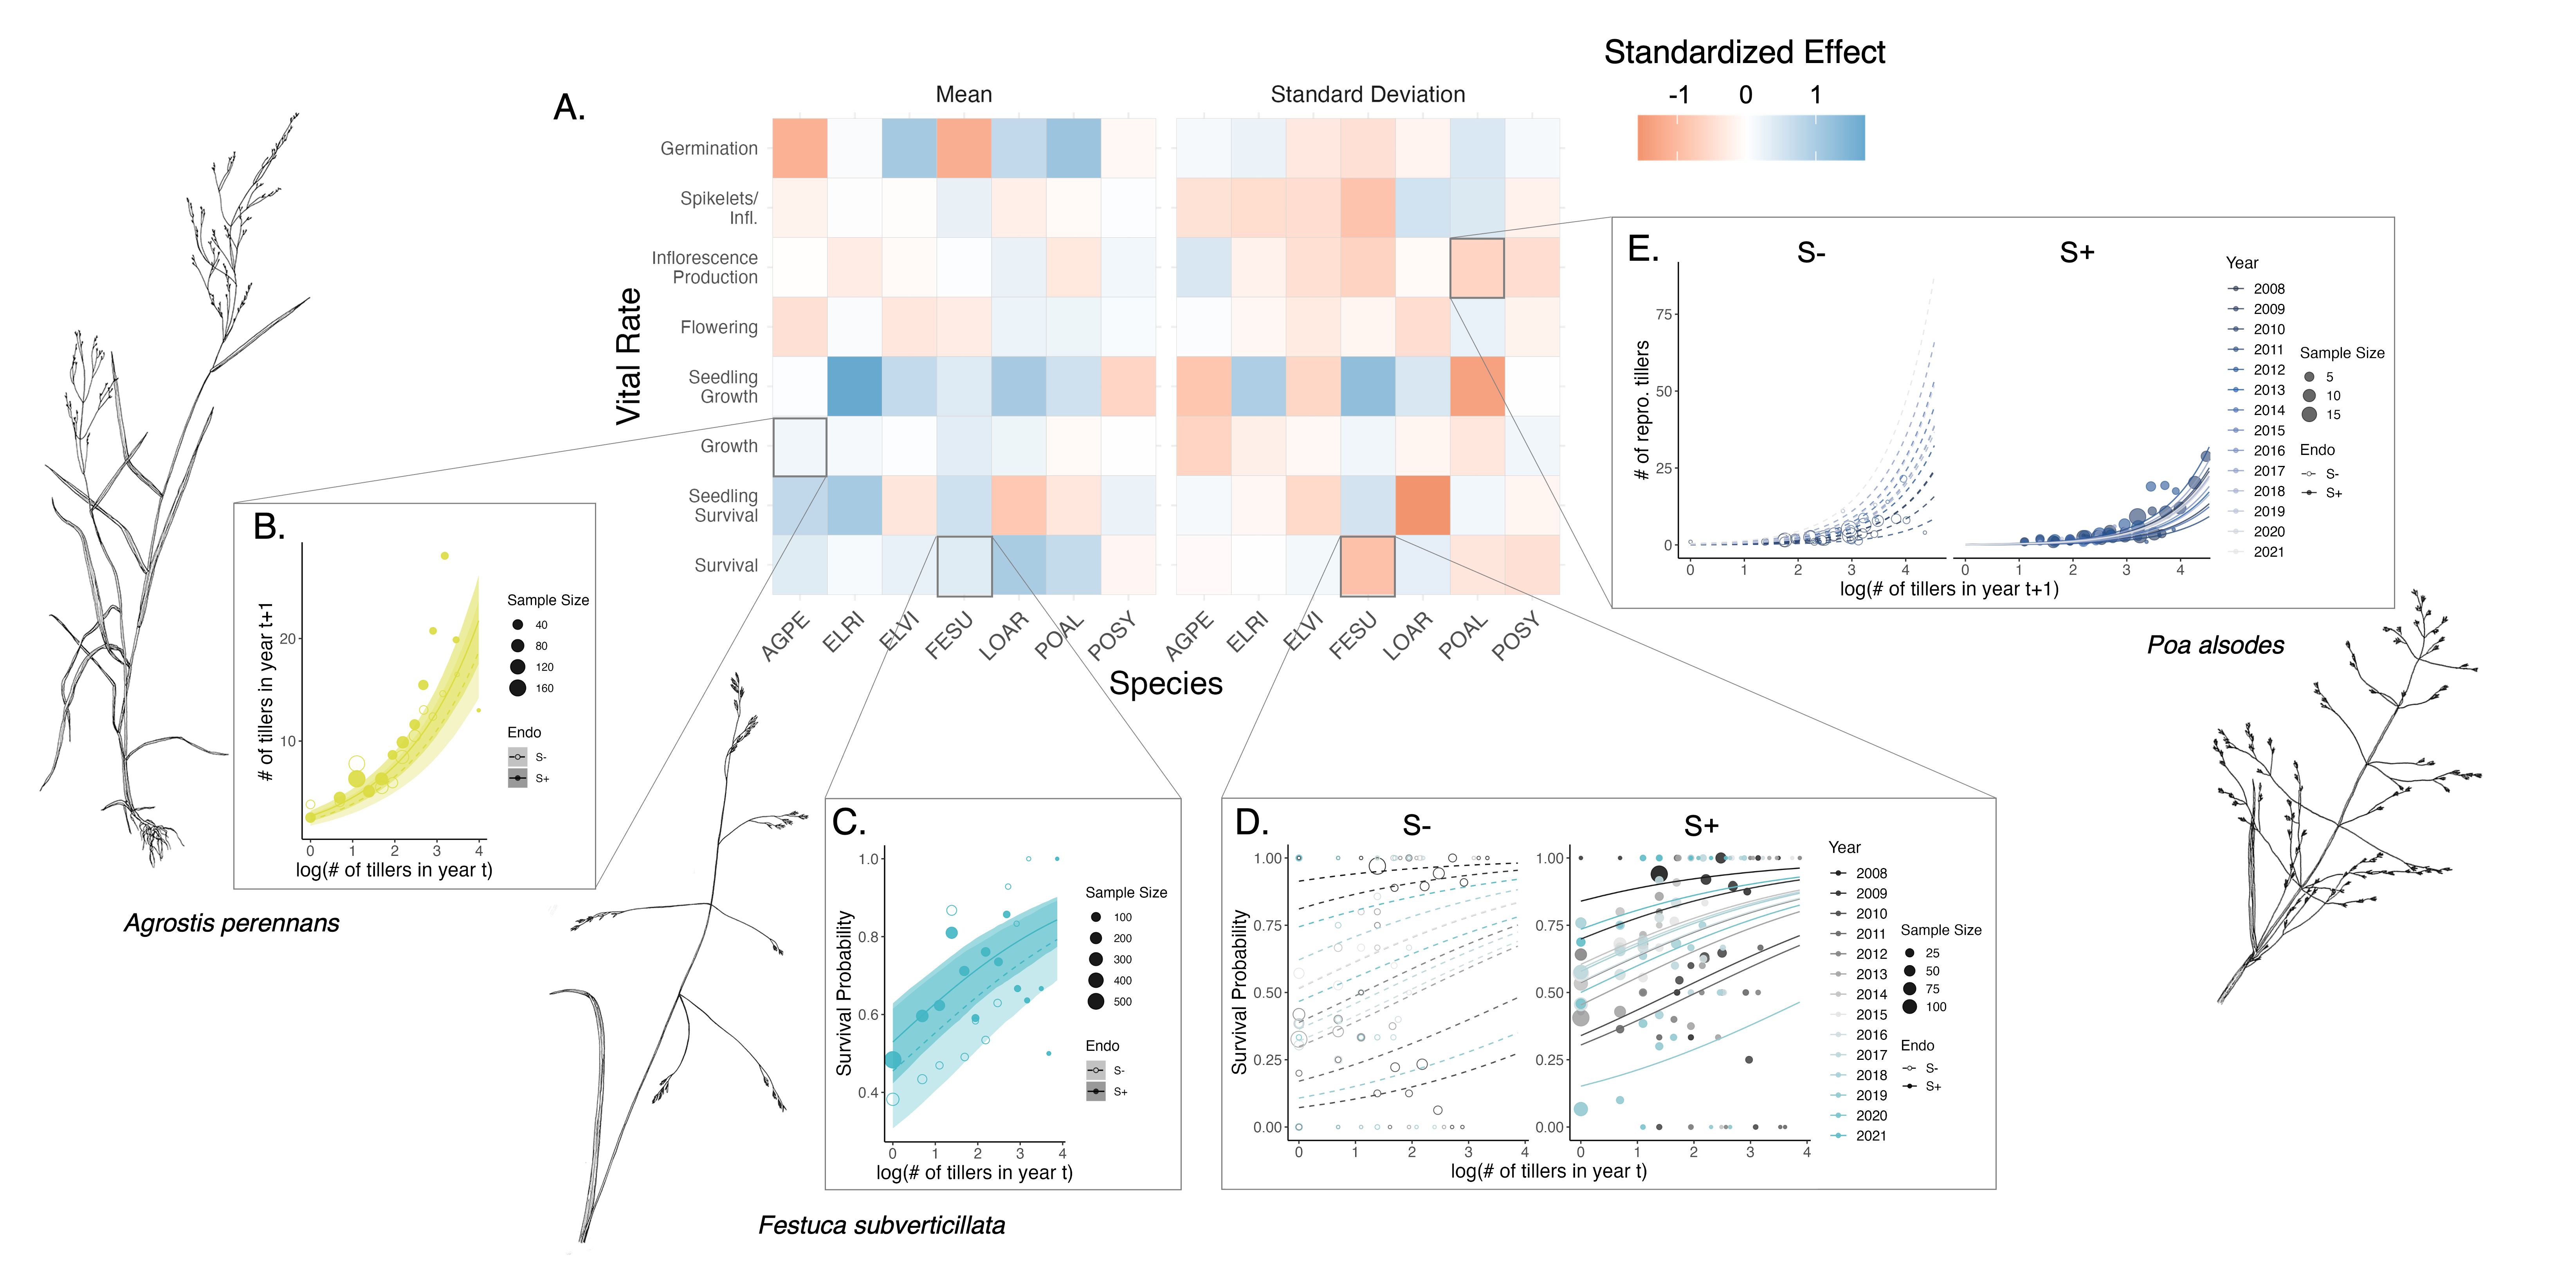
\includegraphics[width=\linewidth]{StochDemo_fig1.png}
\end{figure}
\noindent {\bf Fig. 1.} \textbf{Endophyte symbiosis altered host vital rates.} (A) Shading represents the posterior mean standardized effect size (Cohen's D) of endophyte symbiosis on mean or standard deviation of host vital rates (blue indicates that symbiosis increased the mean or standard deviation and red indicates a reduction). Endophyte presence increased (B) the mean growth of \emph{A. perennans} and (C) the survival probability of \emph{F. subverticillata}. Endophyte presence reduced interannual variance in (D) the survival of \emph{F. subverticillata} and (E) the fertility of \emph{P. alsodes}. Organism silhouettes modified from "Festuca subverticillata" by Cindy Roché and "Agrostis hyemalis" and "Poa alsodes" by Sandy Long © Utah State University)
\newpage

\begin{figure}
	\centering
	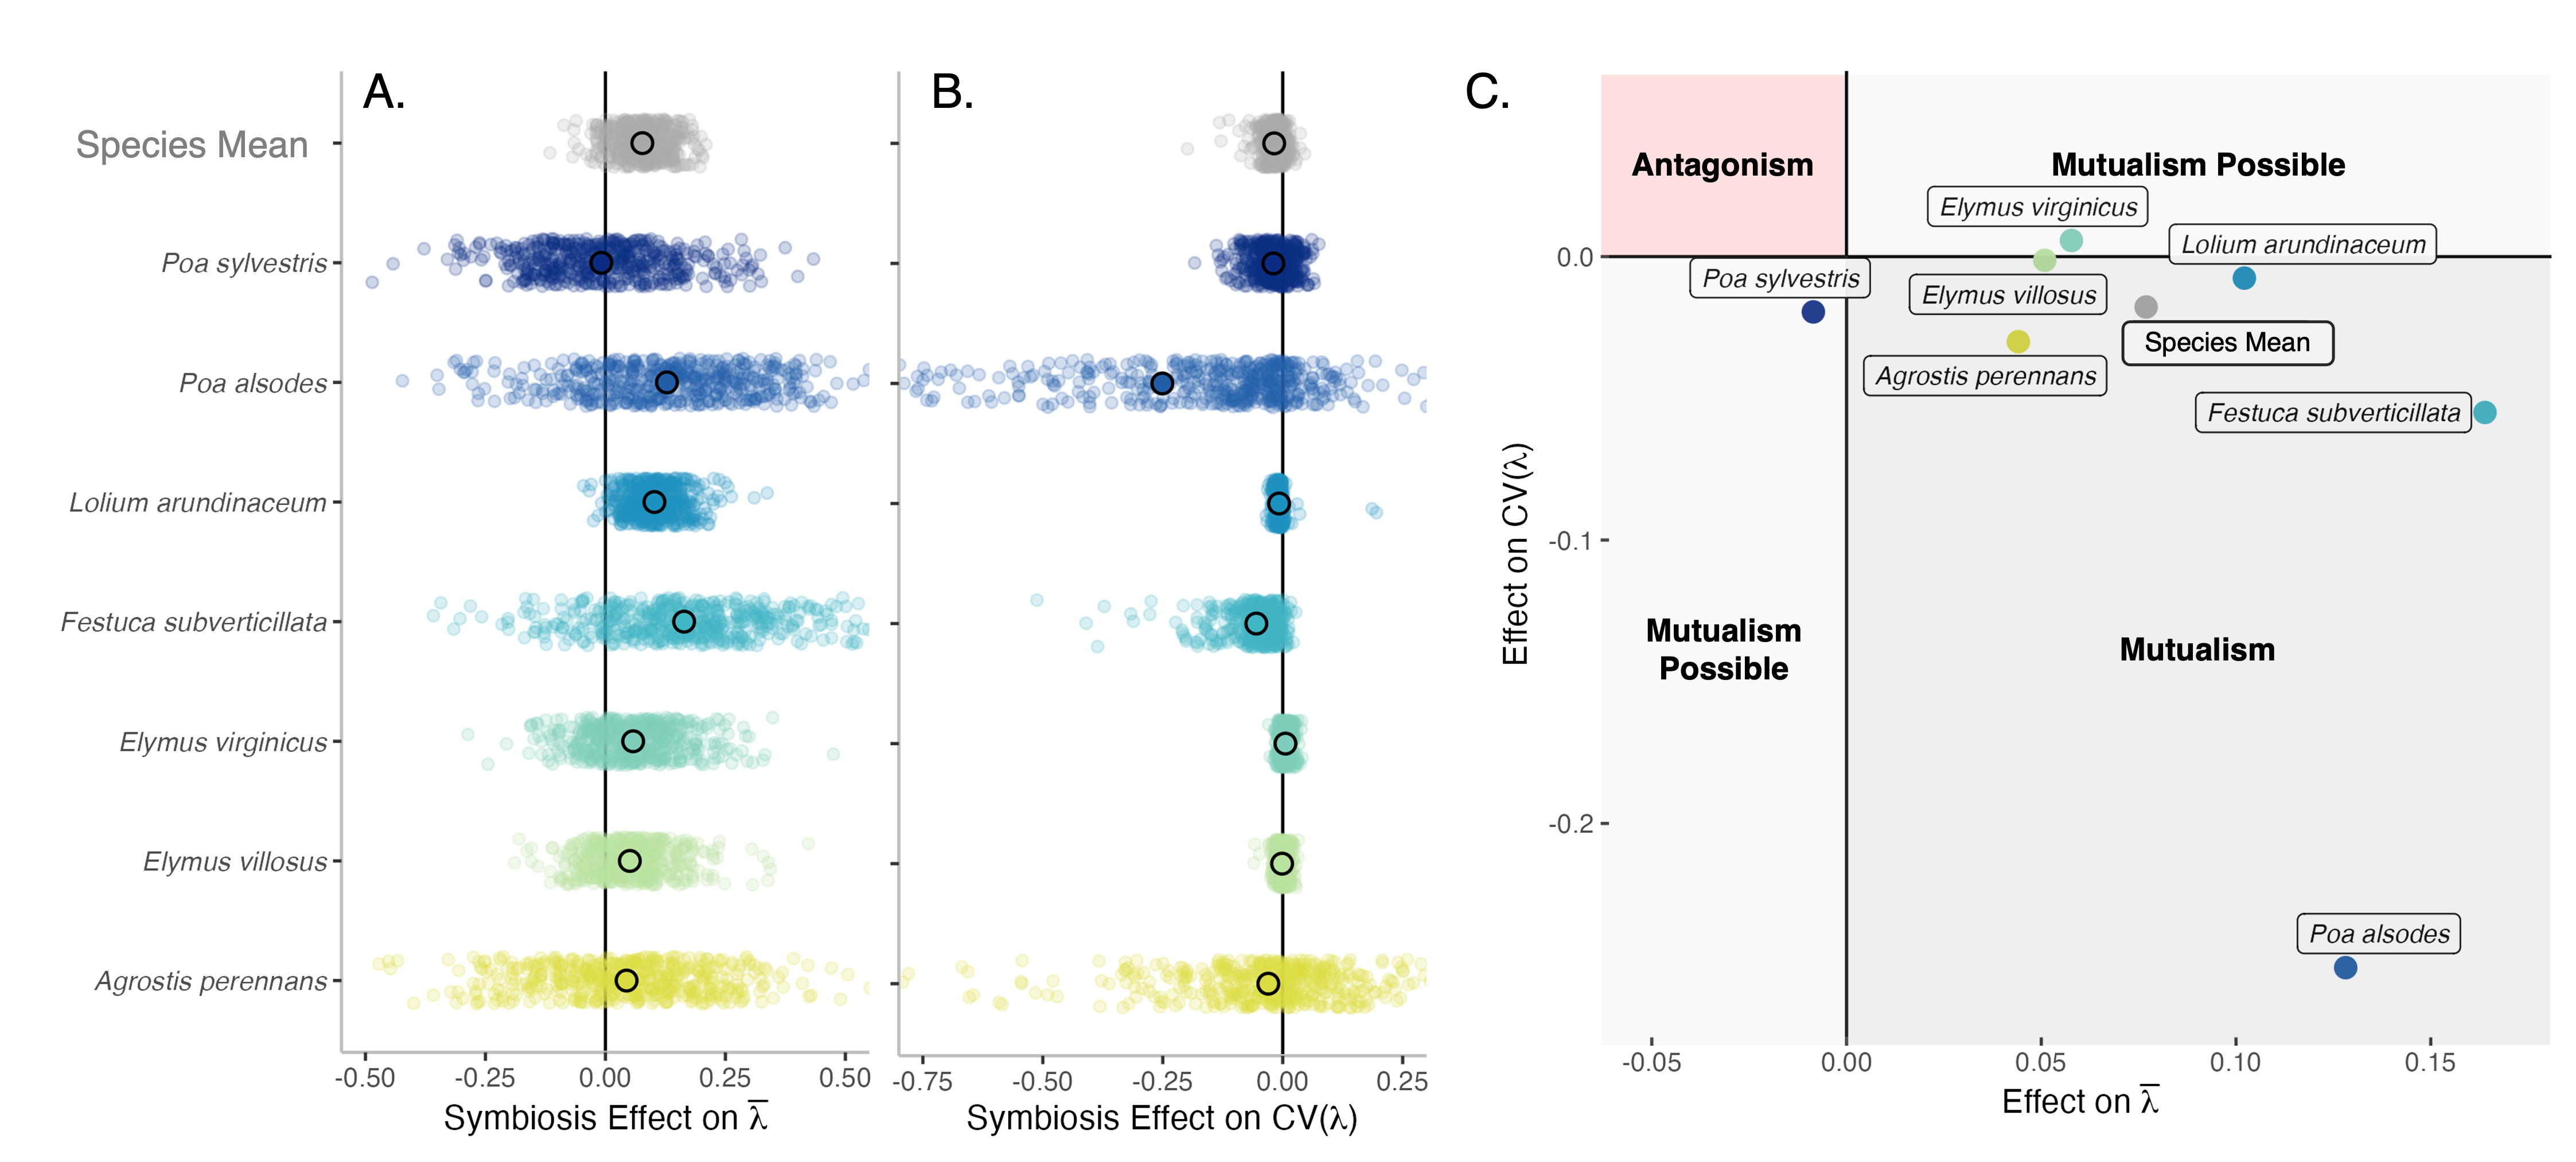
\includegraphics[width=\linewidth]{StochDemo_fig2.png}
\end{figure}
\noindent {\bf Fig. 2.} \textbf{Mean and variance-buffering effects on population growth rates.} Black circles indicate the average effect of endophytes along with 500 posterior draws (smaller colored circles) on the (A) mean and (B) coefficient of variation in population growth rates $\lambda$ for each host species as well as a cross species mean. (C) For all hosts, endophytes either reduce variance, increase the mean, or both, and consequently when considering stochastic environments, the interactions are always at least potentially mutualistic.
\newpage

\begin{figure}
	\centering
	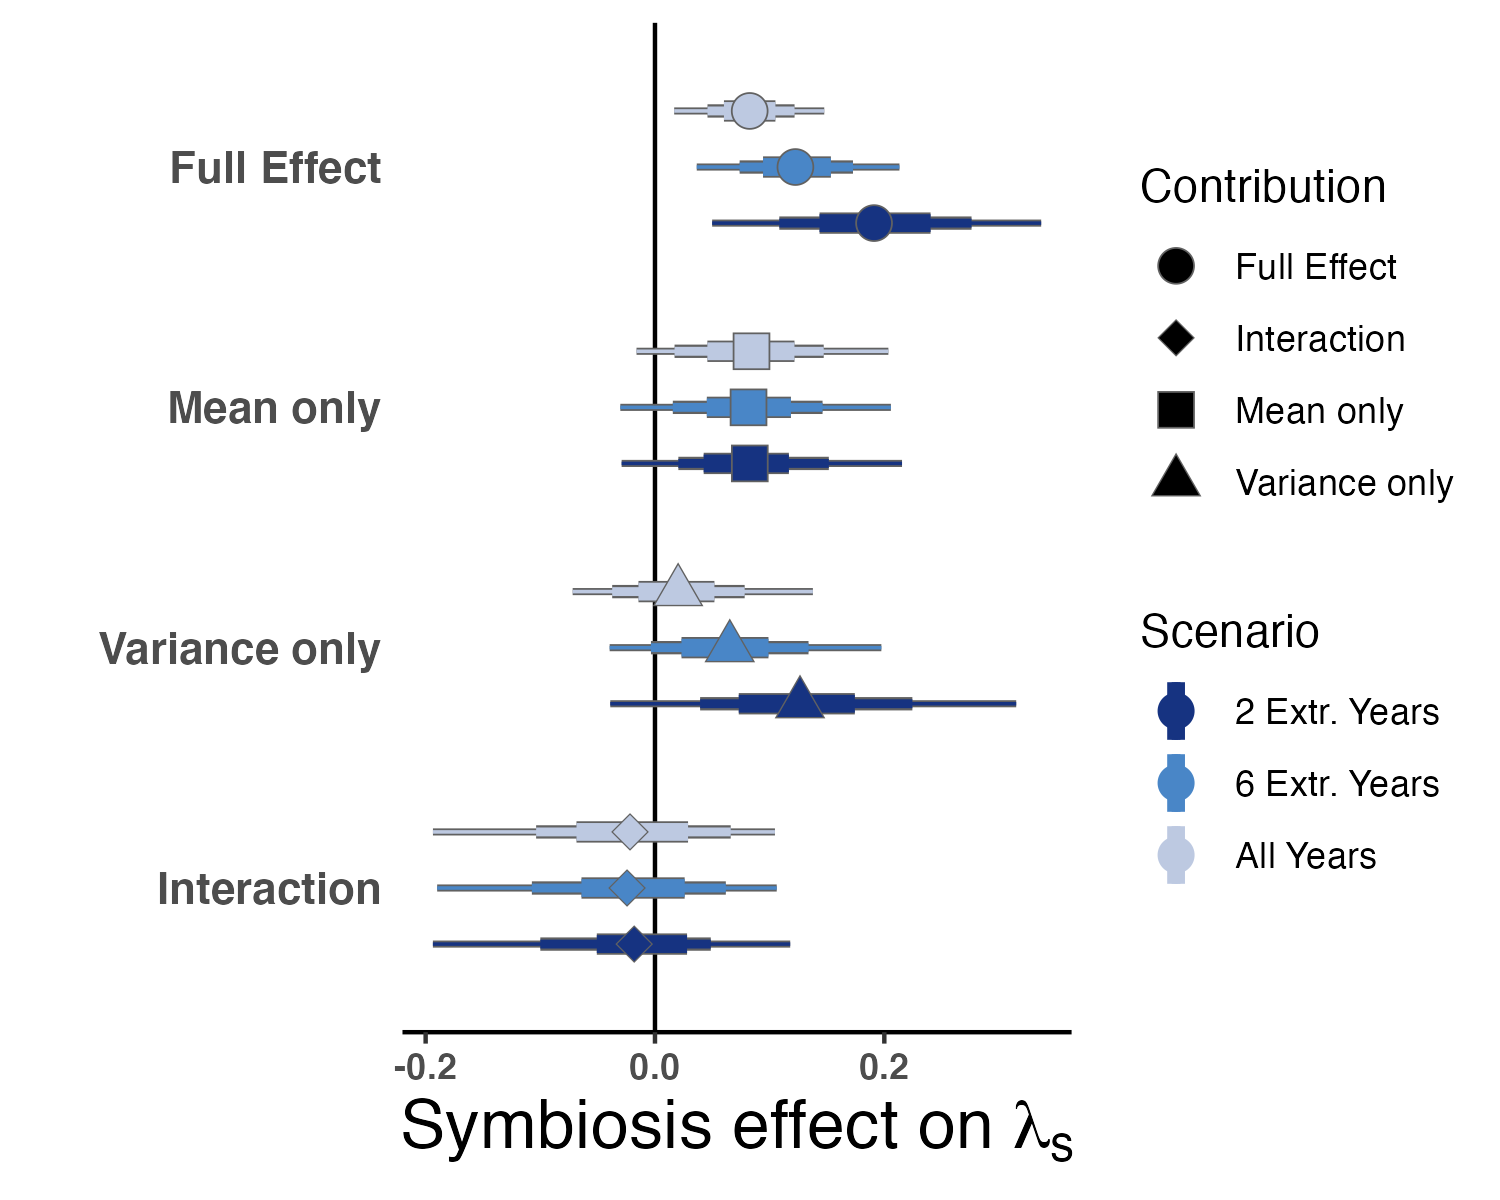
\includegraphics[width=\linewidth]{StochDemo_fig3.png}
\end{figure}
\noindent {\bf Fig. 3.} \textbf{Host species with faster life history traits experience stronger effects of symbiont-mediated variance buffering.} Regressions between life history traits describing the fast-slow life history continuum ((A) Maximum age observed during long term censuses; (B) 99th percentile maximum age during demographic censuses; (C) Net reproductive rate; (D) Longevity; (E) Mean life expectancy; (F) Generation time; (G) Seed size; (H) Rate of imperfect transmission) and the effect of endophyte symbiosis on the coefficent of variation in population growth rate ($\lambda$). Each panel shows the fitted mean relationship (line) along with the 95\% credible interval.
\newpage


\begin{figure}
	\centering
	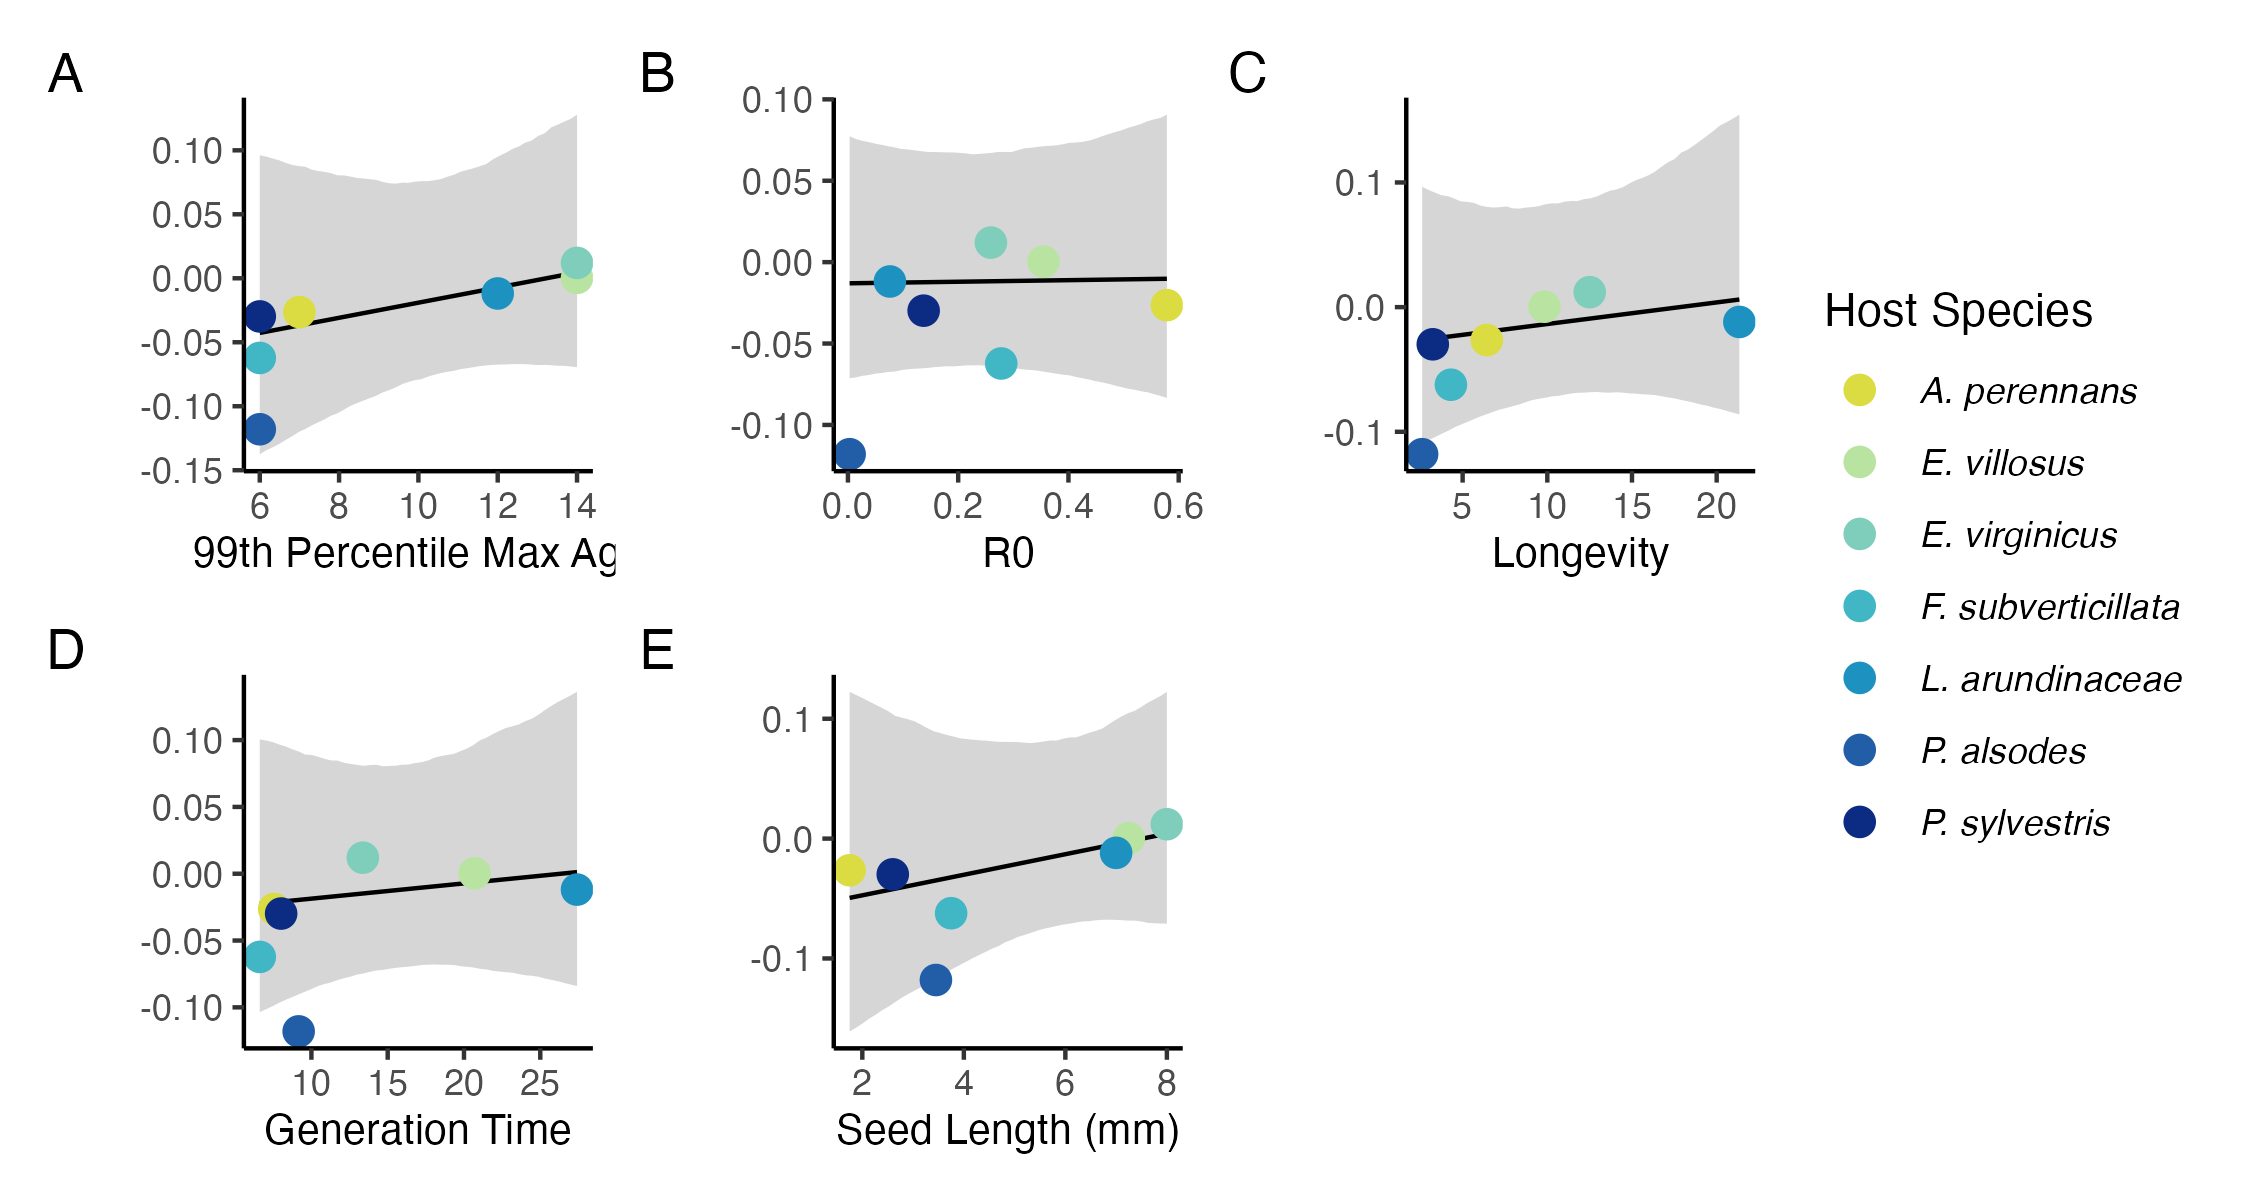
\includegraphics[width=.8\linewidth]{StochDemo_fig4.png}
\end{figure}
\noindent {\bf Fig. 4.} \textbf{Cross-species average endophyte contributions to stochastic growth rates under observed and elevated variance.} Endophyte symbiosis contributes to the total effect of mutualism through benefits to mean growth rates and through variance buffering as well as the interaction between mean and variance effects. Shapes indicate the posterior mean of each contribution averaged across the seven focal symbiota, along with bars for the 50, 75 and 95 \% credible intervals.  The full effect of the symbiosis (circles) becomes more mutualistic under scenarios of increased variance (represented by color intensity). Relative to a scenario sampling transition matrices for all 14 years during the study period, simulations increased variance by sampling the most extreme six or two years, leading to increased contributions from variance buffering effects (triangles) and a constant contribution from mean effects (squares).
\newpage





\begin{figure}[H]
	\centering
	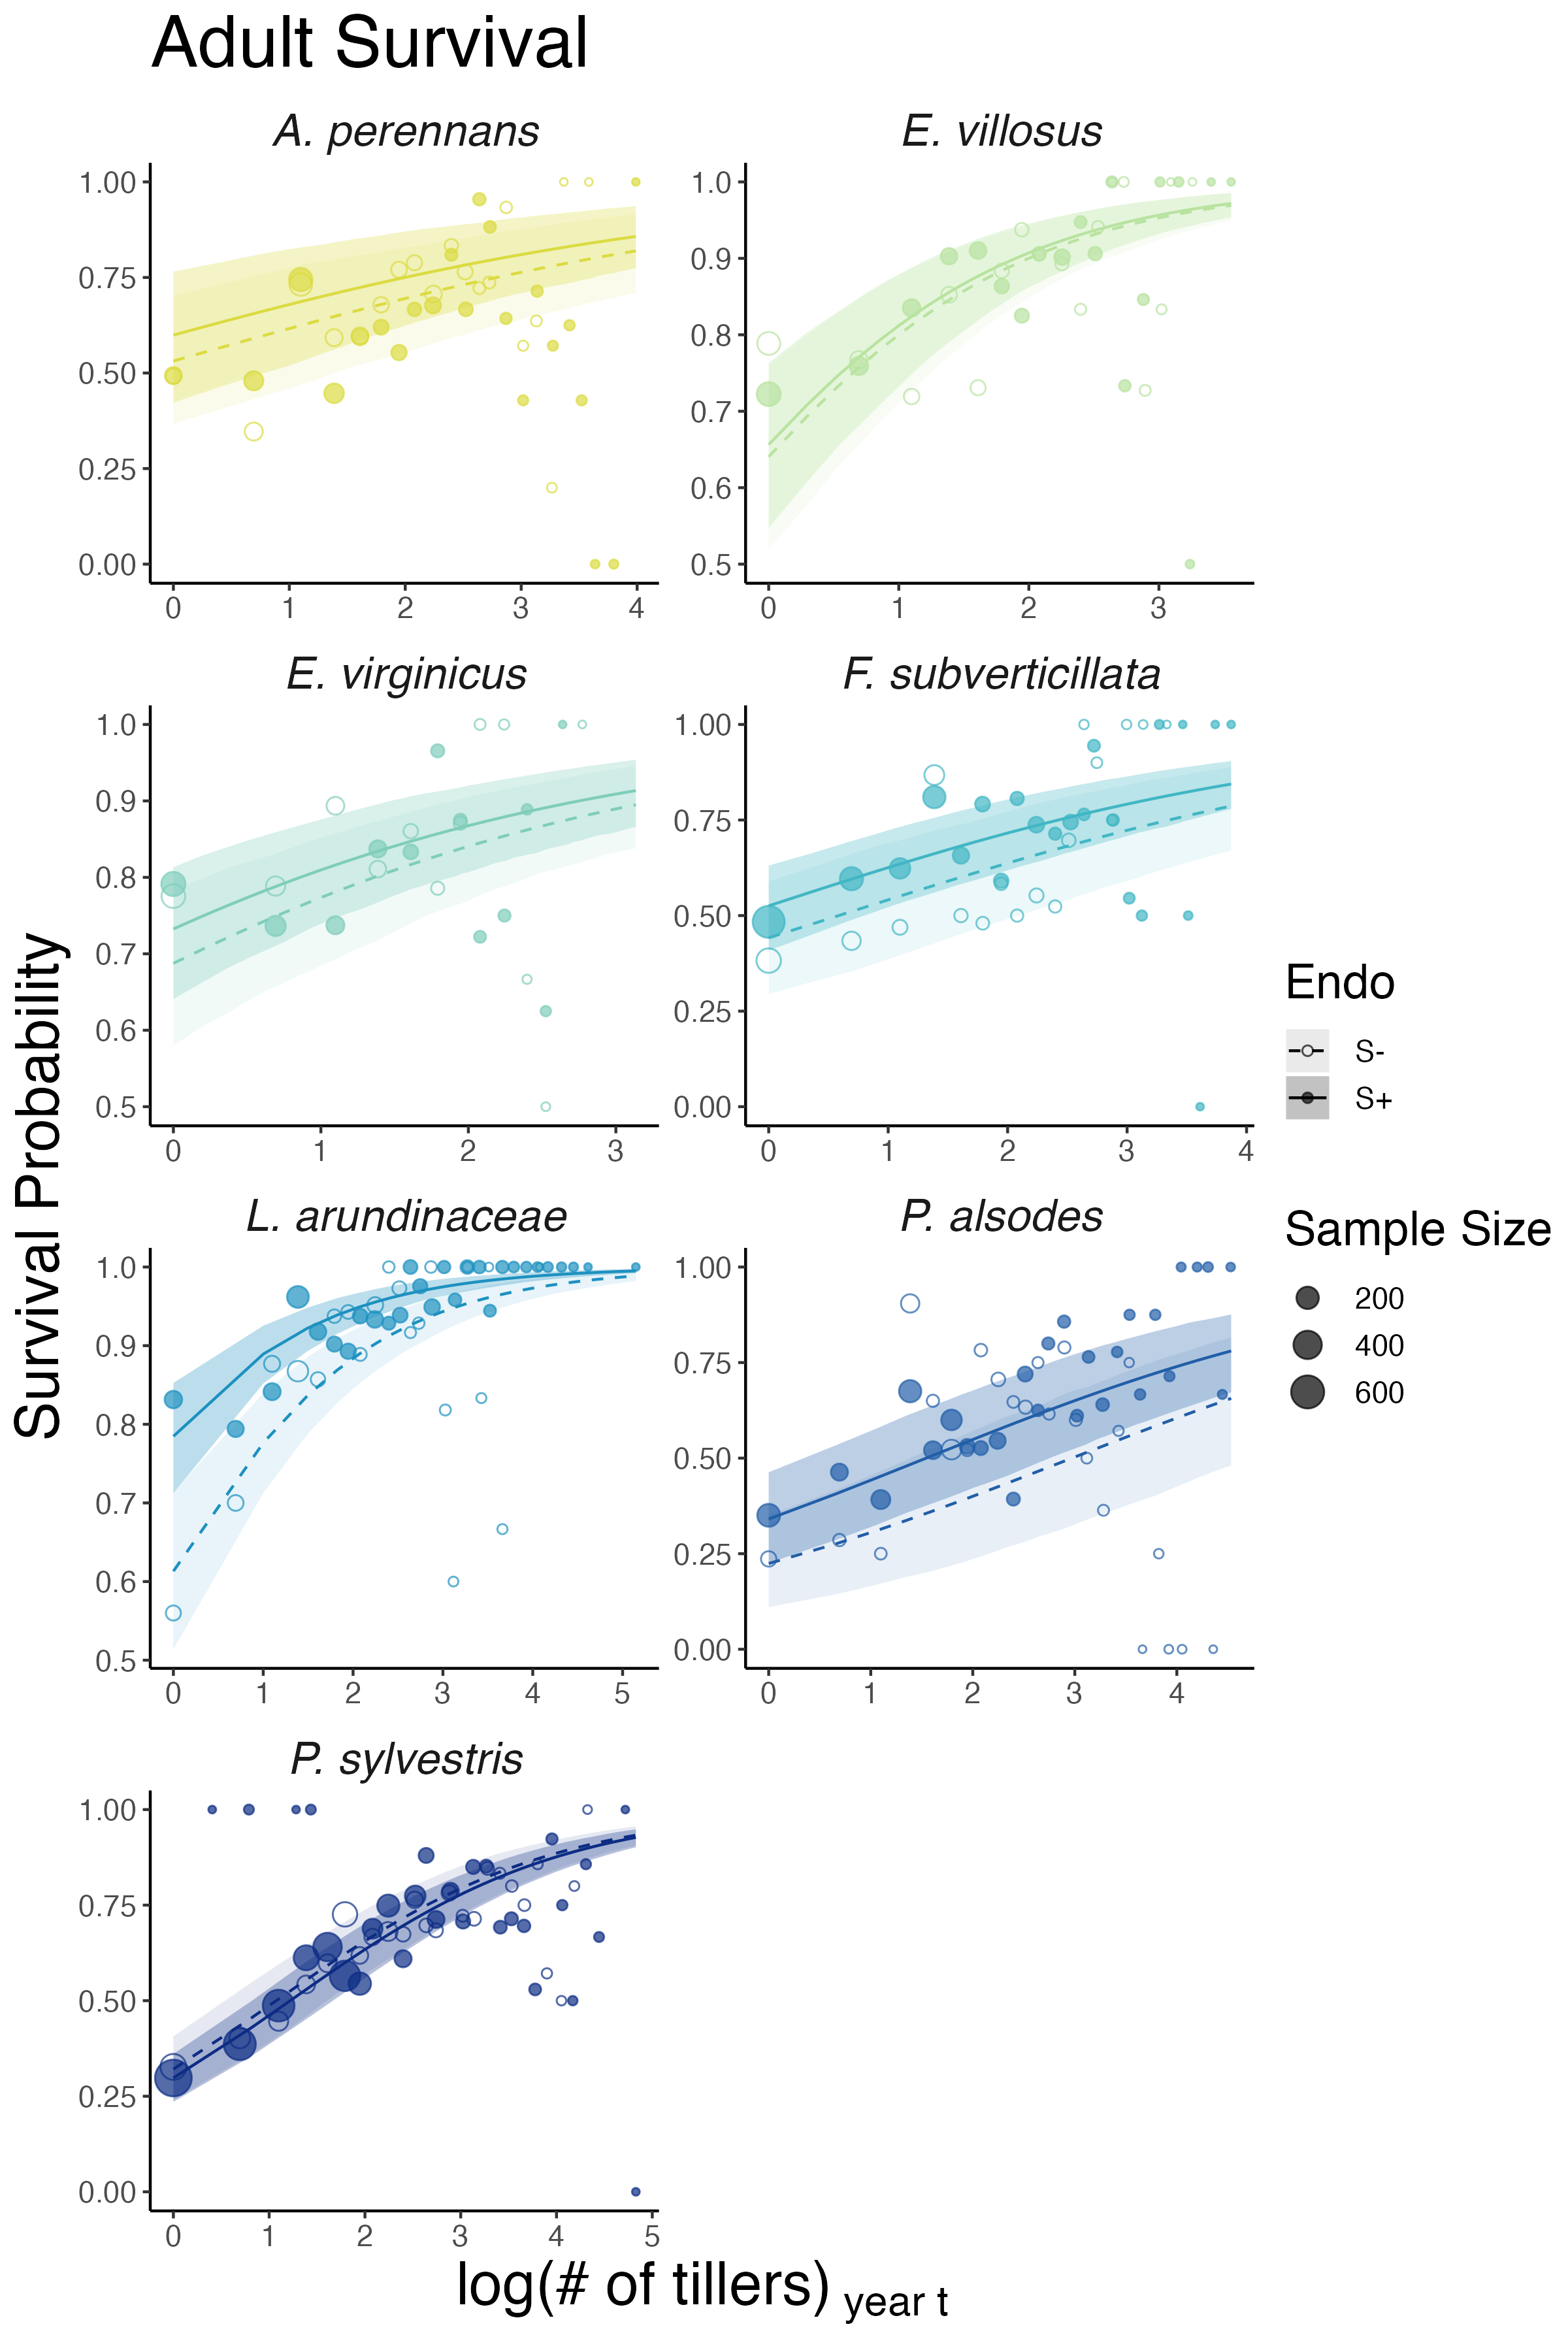
\includegraphics[width=.8\linewidth]{surv_meanplot.png}
\end{figure}
\noindent {\bf Fig. S1.} \textbf{Effect of endophyte symbiosis on the mean value of adult survival.} Fitted curves represent the size-specific mean survival probability along with data binned by size shown as open circles with a dashed line for symbiont-free (S-) plants , while the solid line and filled circles represent symbiontic (S+) plants. 80\% credible intervals are shown with dark shading for  S+, or light shading for S-.
\begin{figure}[H]
	\centering
	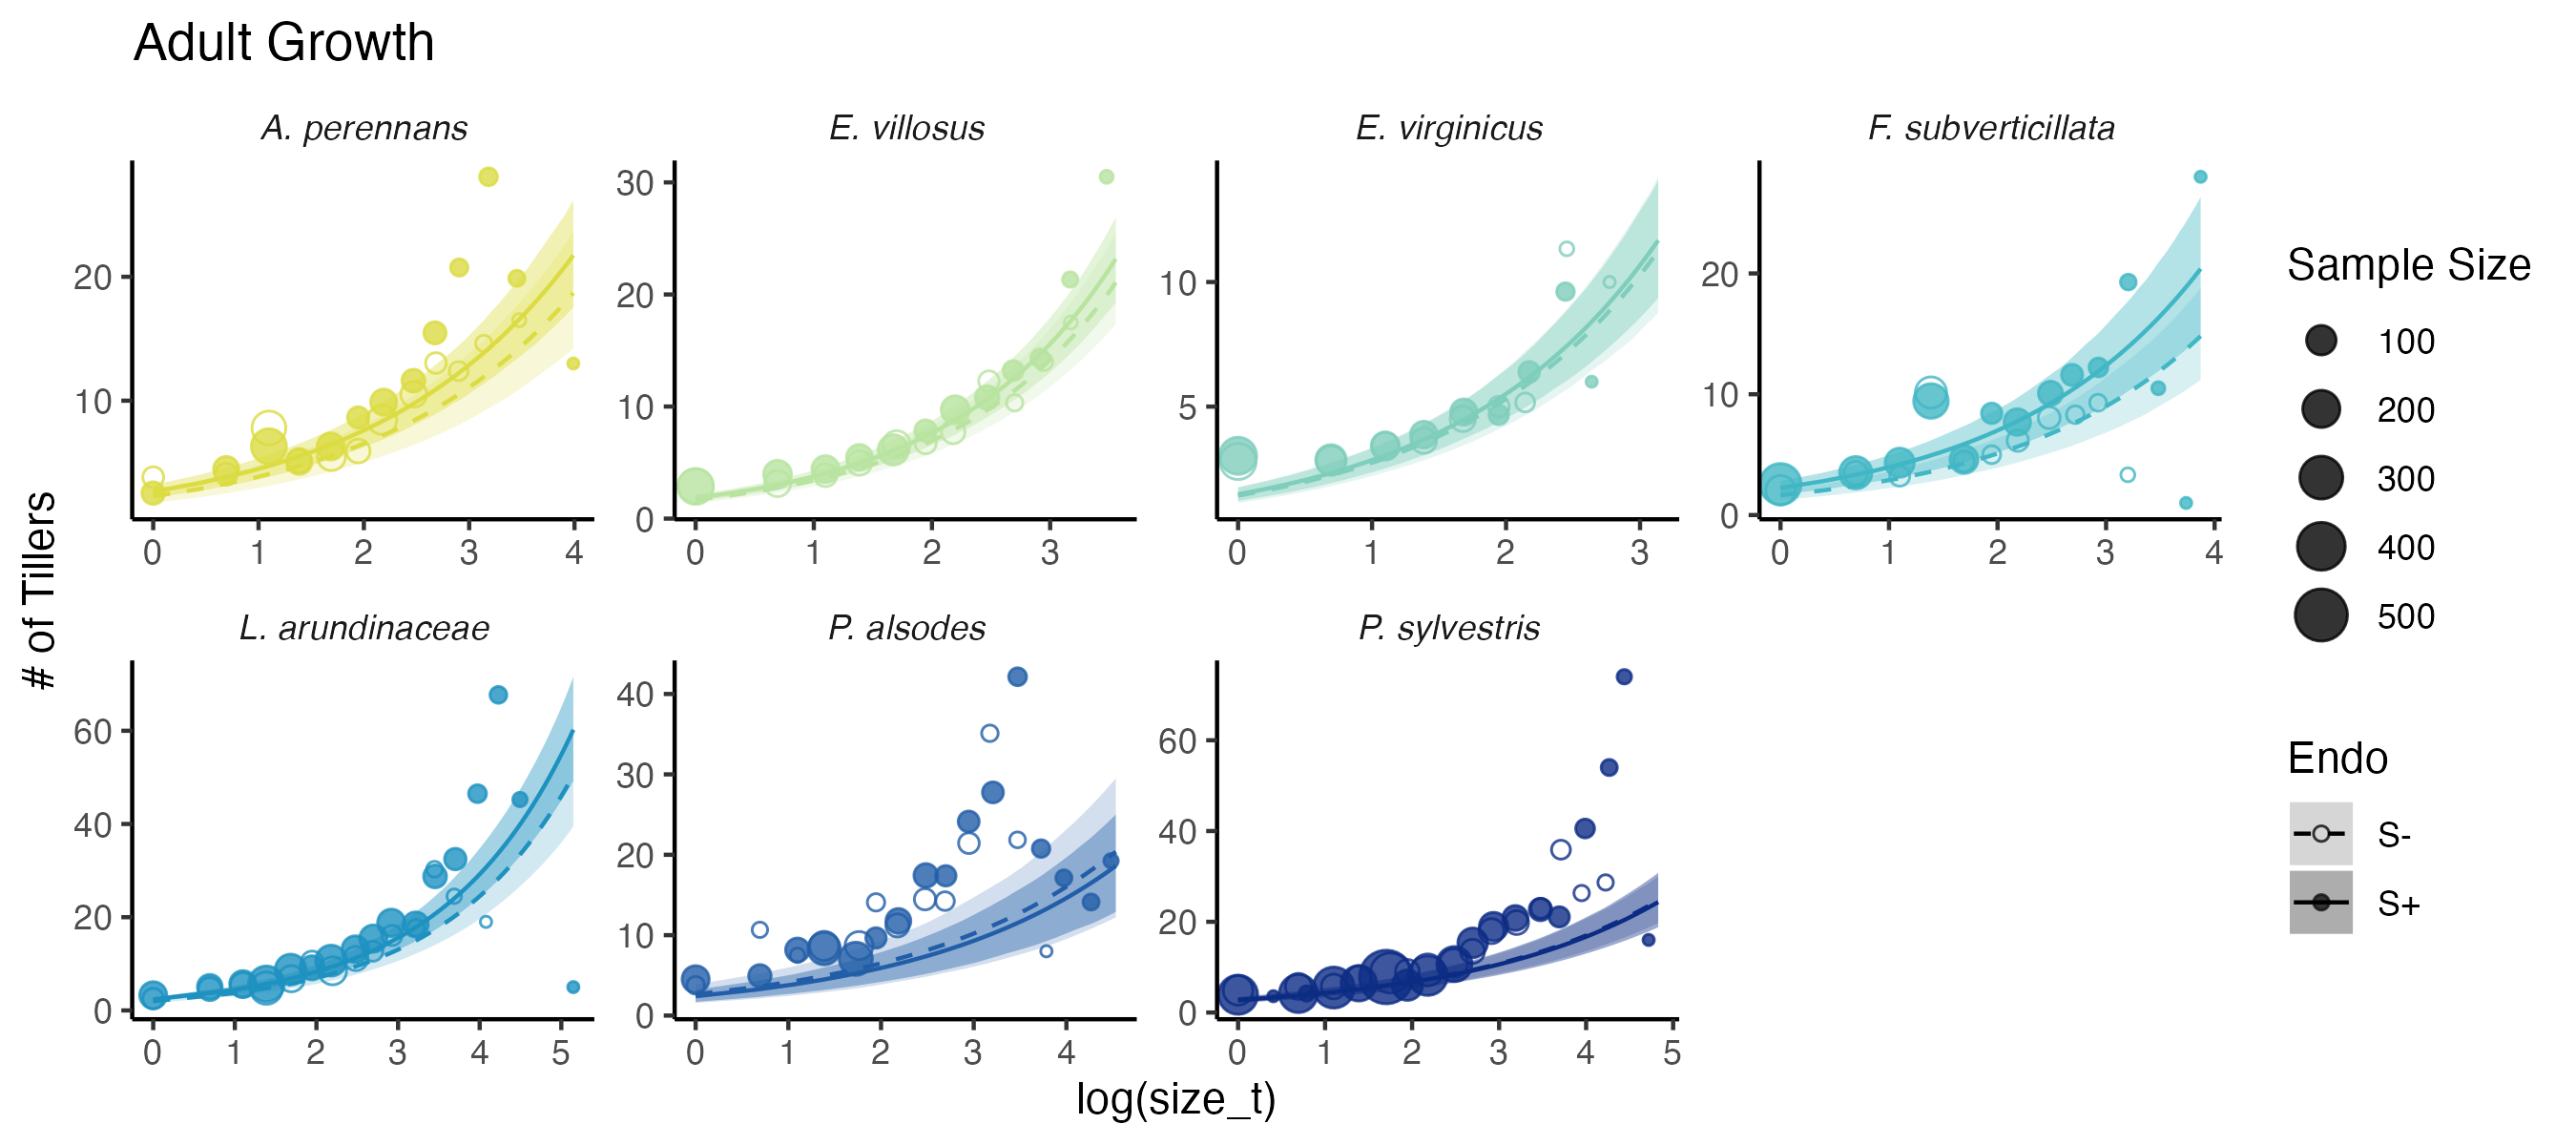
\includegraphics[width=.8\linewidth]{grow_meanplot.png}
\end{figure}
\noindent {\bf Fig. S2.} \textbf{Effect of endophyte symbiosis on the mean value of adult growth.} Fitted curves represent the size-specific mean expected plant size along with data binned by size shown as open circles with a dashed line for symbiont-free (S-) plants , while the solid line and filled circles represent symbiontic (S+) plants. 80\% credible intervals are shown with dark shading for  S+, or light shading for S-.
\newpage

\begin{figure}[H]
	\centering
	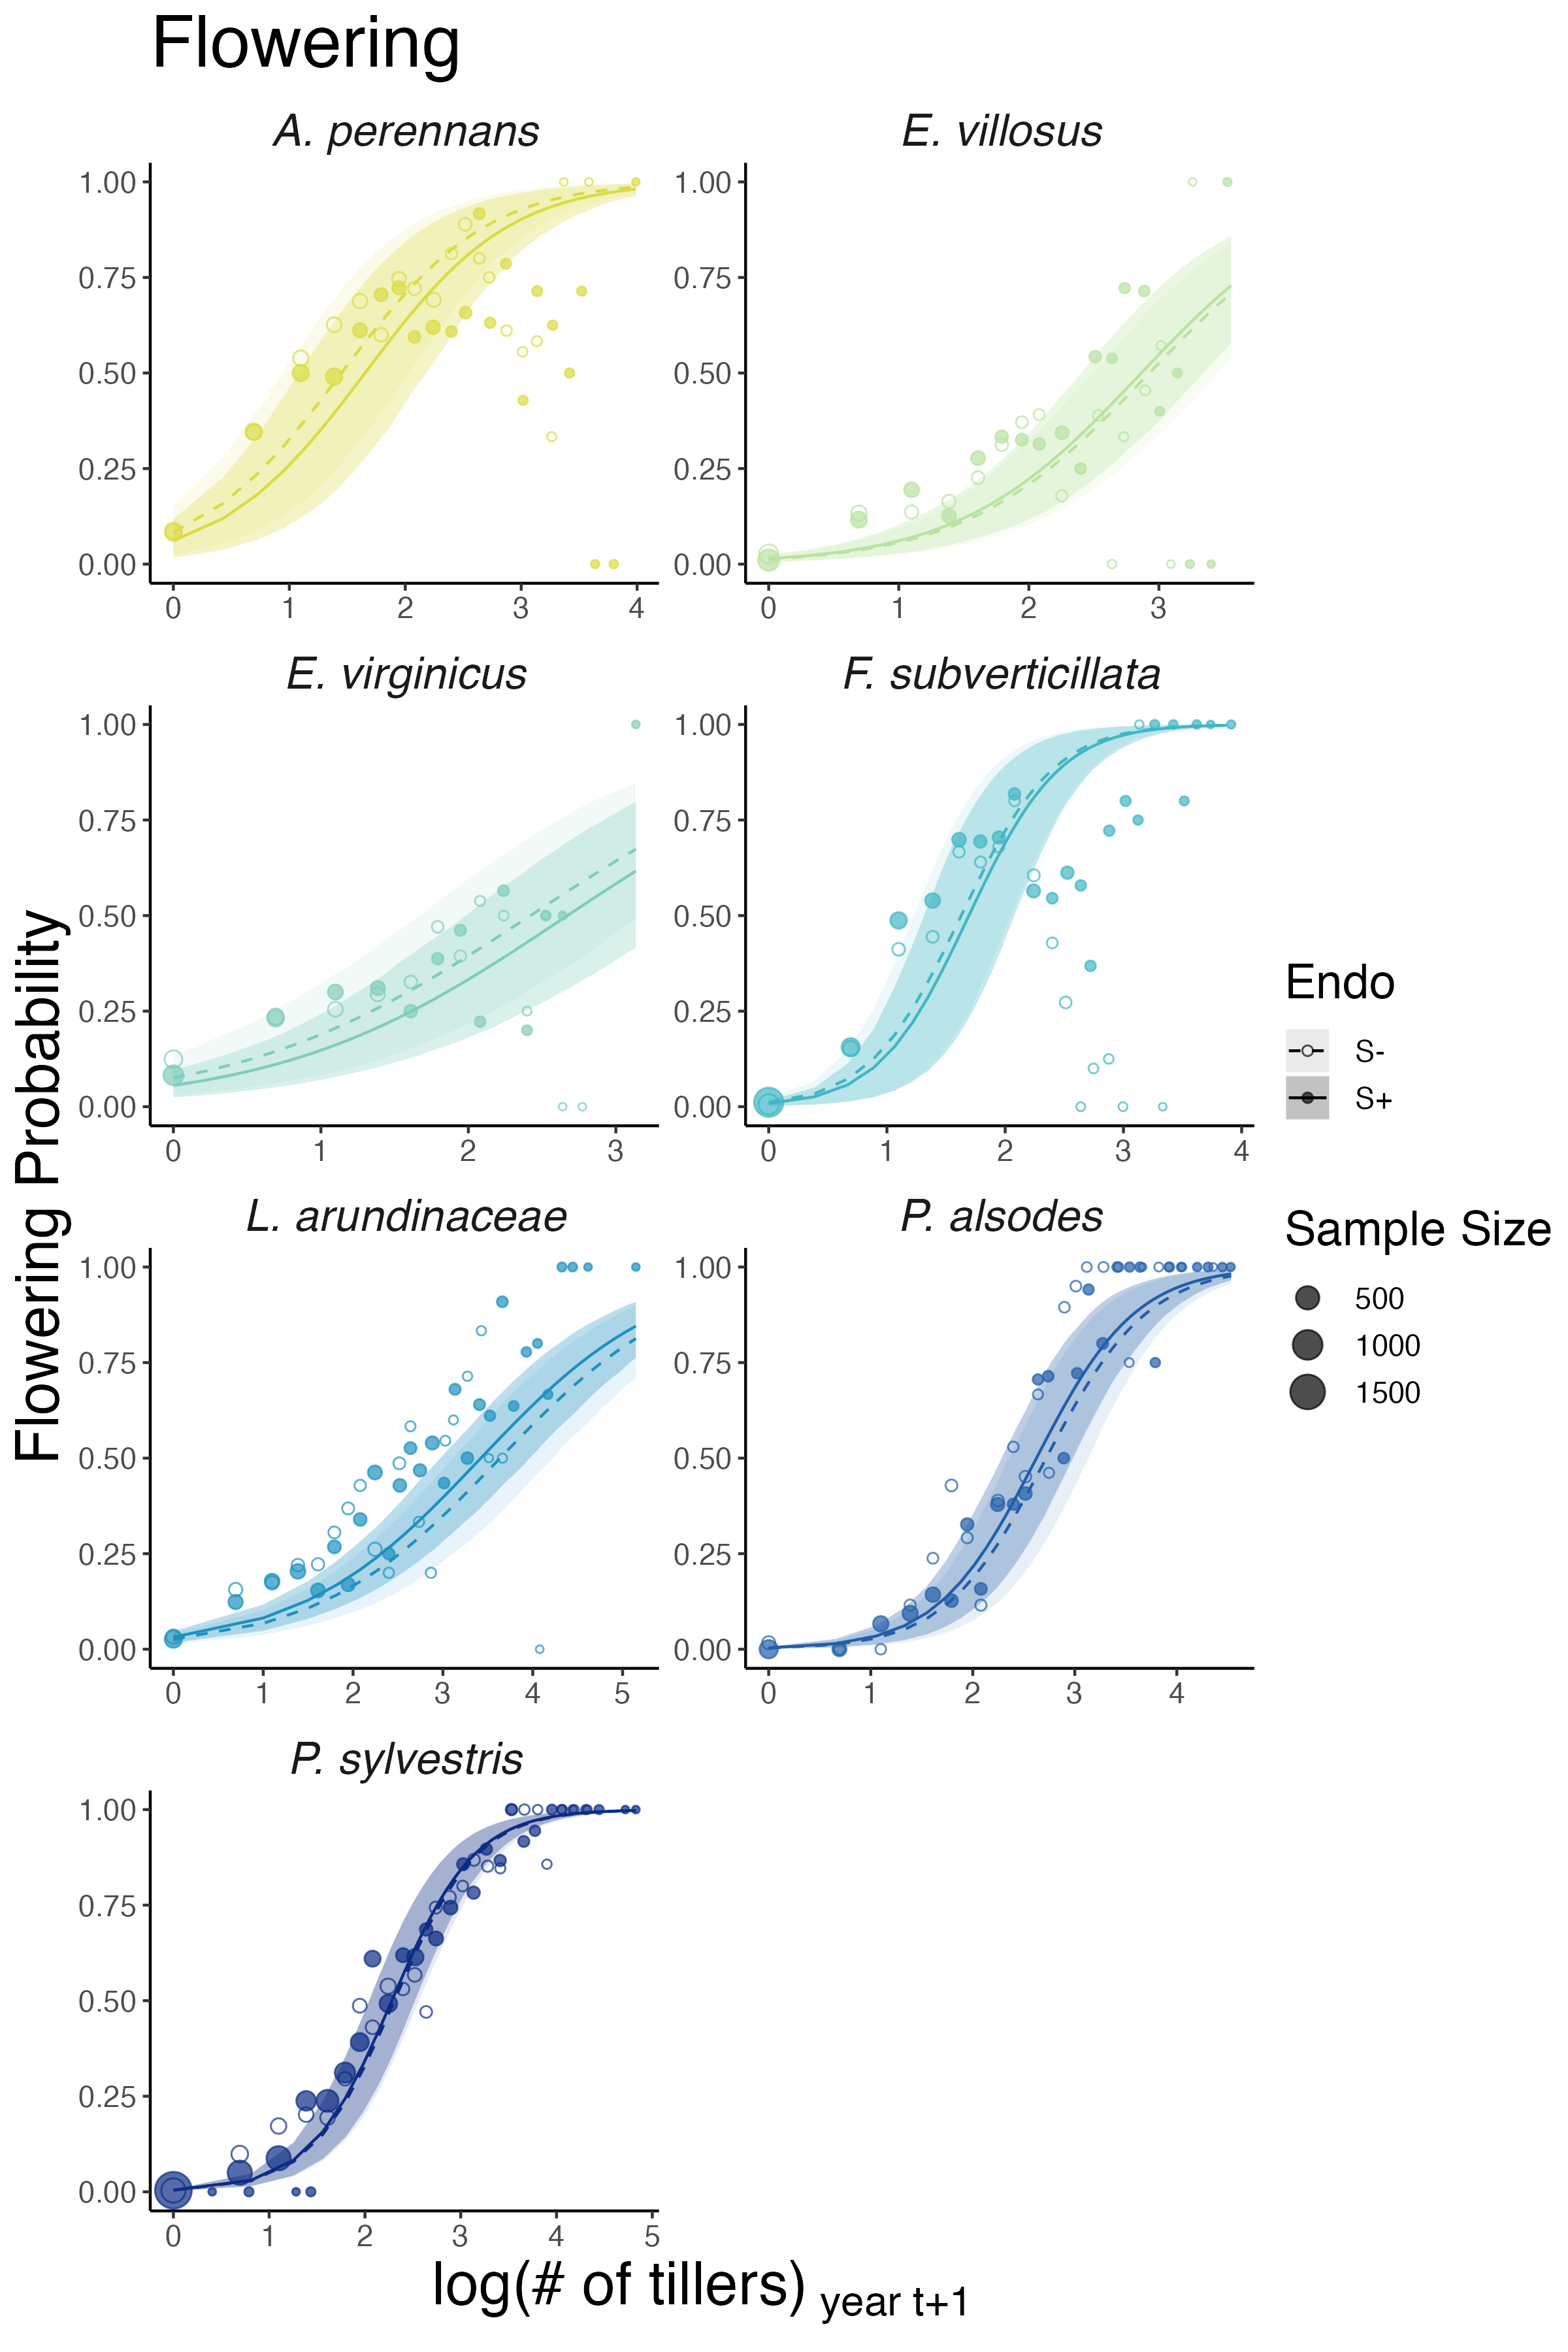
\includegraphics[width=.8\linewidth]{flw_meanplot.png}
\end{figure}
\noindent {\bf Fig. S3.} \textbf{Effect of endophyte symbiosis on the mean value of flowering} Fitted curves represent the size-specific mean flowering probability along with data binned by size shown as open circles with a dashed line for symbiont-free (S-) plants , while the solid line and filled circles represent symbiontic (S+) plants. 80\% credible intervals are shown with dark shading for  S+, or light shading for S-.
\begin{figure}[H]
	\centering
	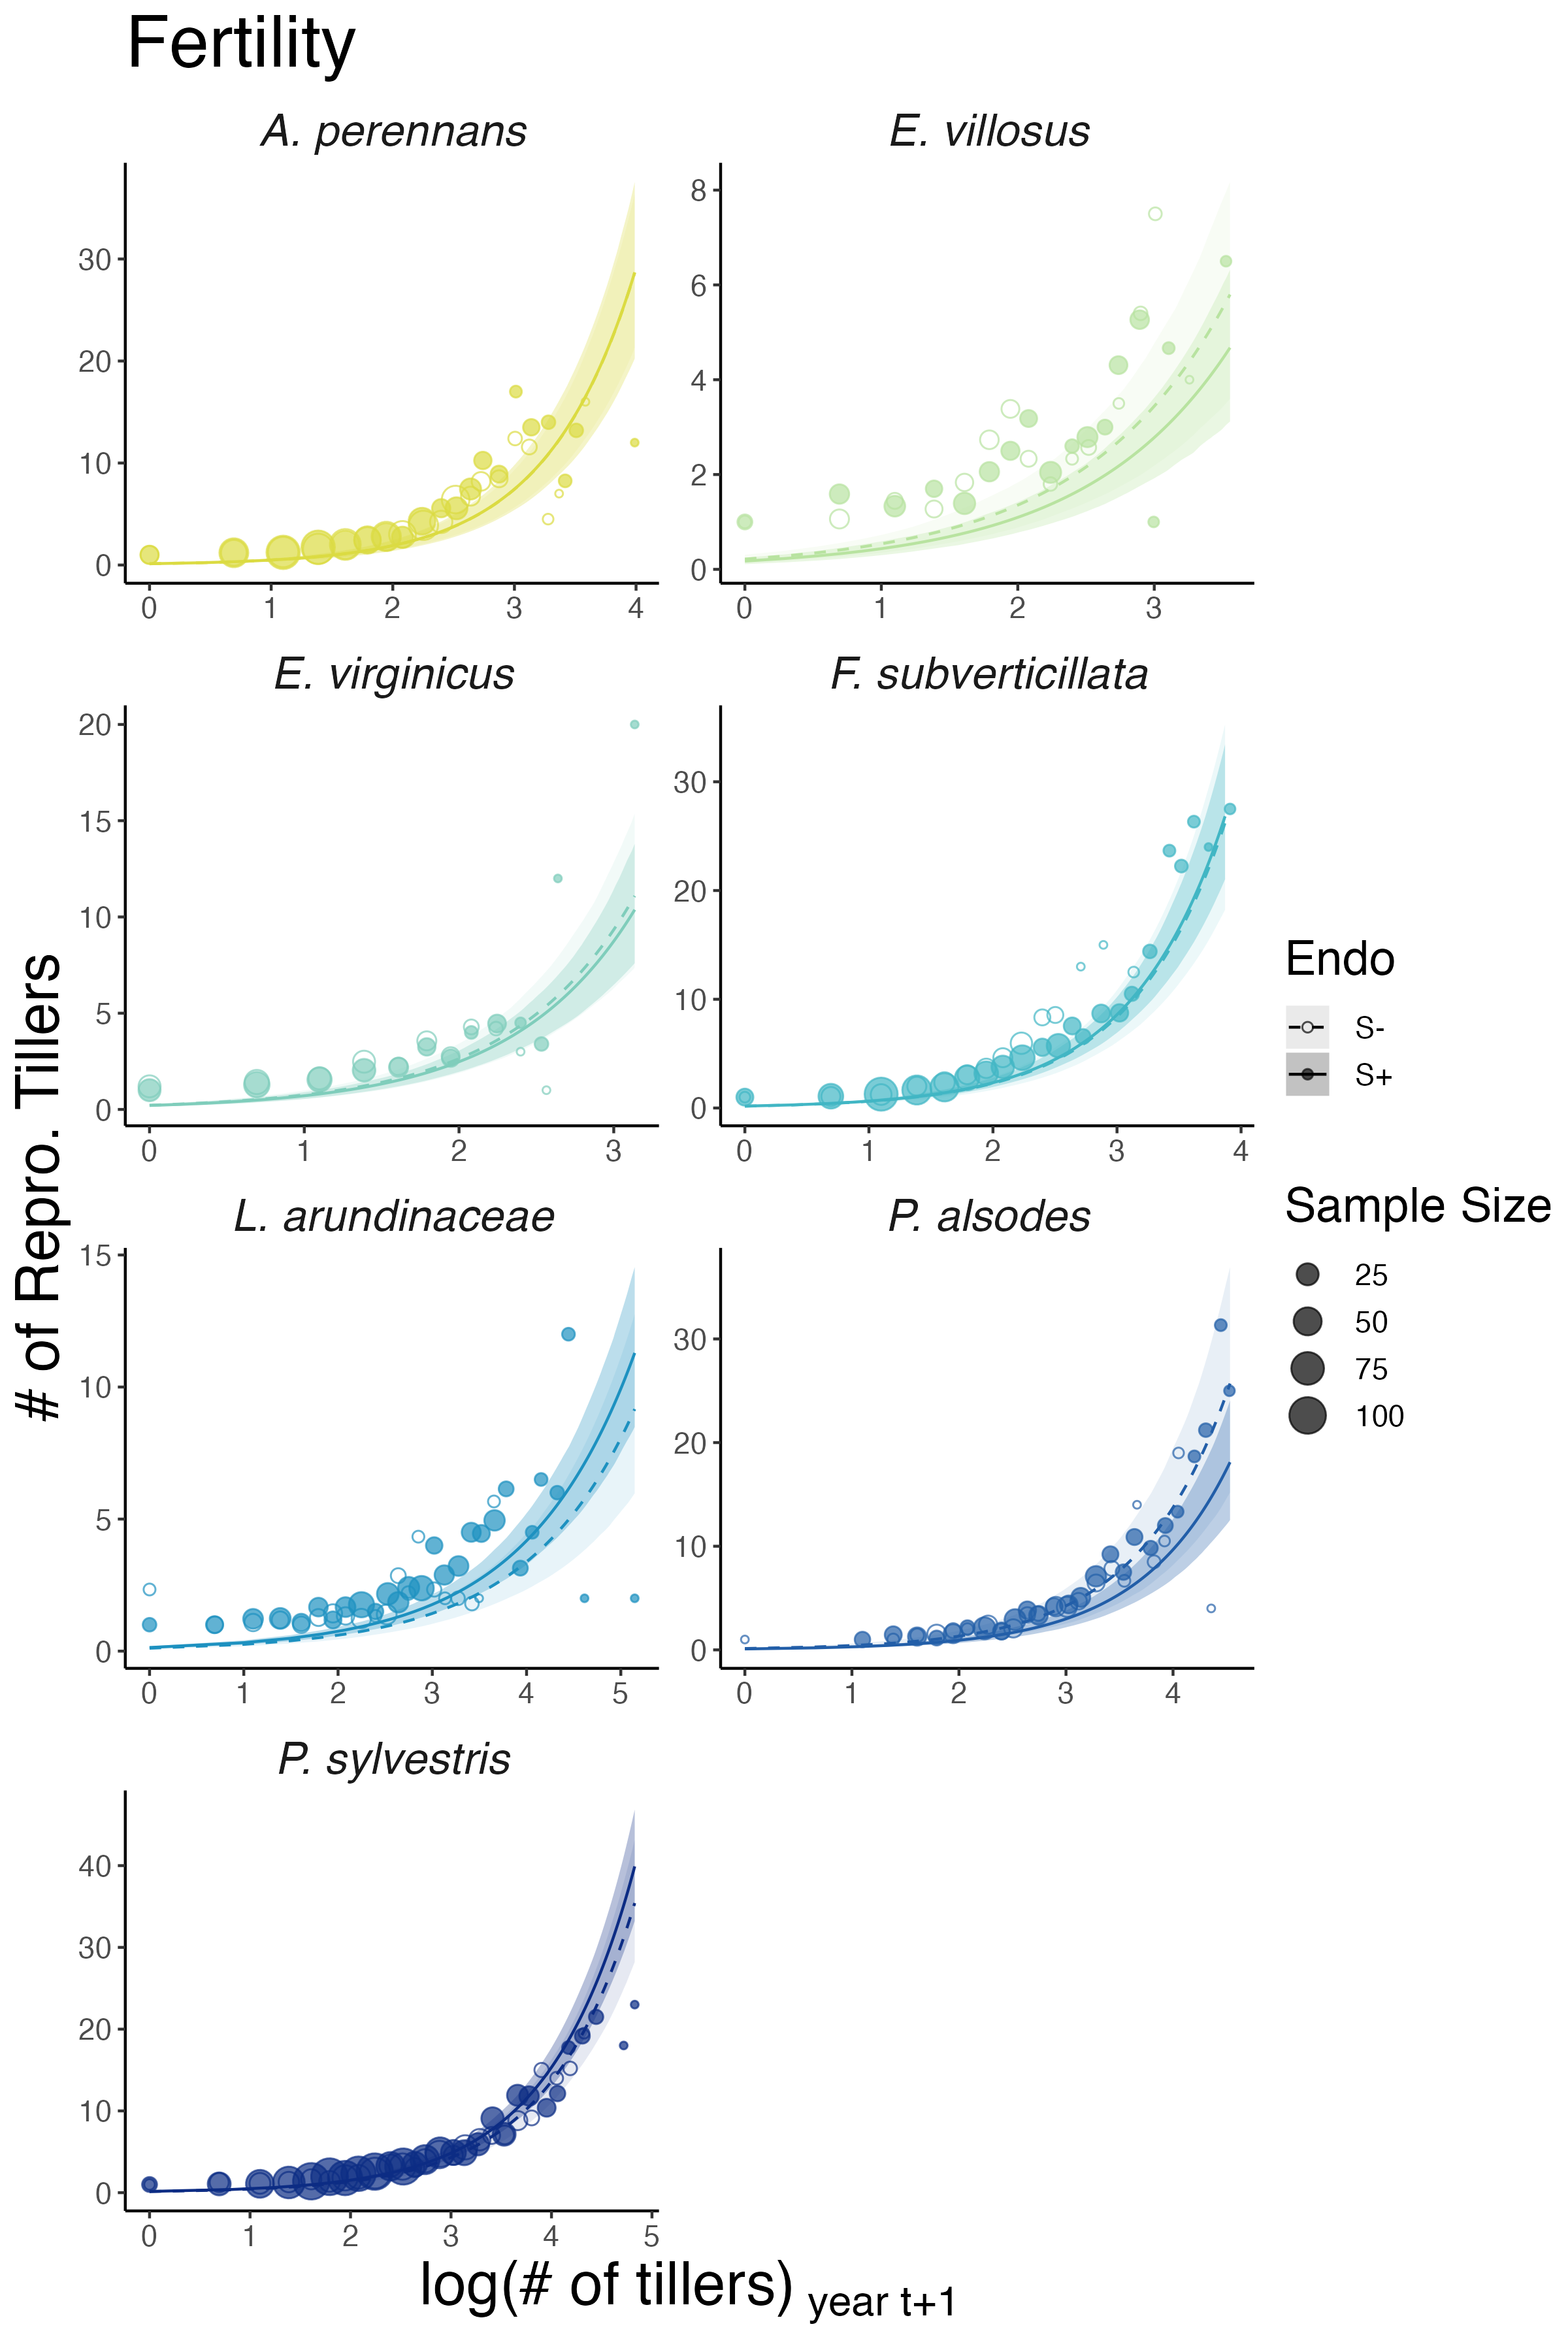
\includegraphics[width=.8\linewidth]{fert_meanplot.png}
\end{figure}
\noindent {\bf Fig. S4.} \textbf{Effect of endophyte symbiosis on the mean value of fertility.} Fitted curves represent the size-specific mean expected number of flowering tillers along with data binned by size shown as open circles with a dashed line for symbiont-free (S-) plants , while the solid line and filled circles represent symbiontic (S+) plants. 80\% credible intervals are shown with dark shading for  S+, or light shading for S-.
\newpage
\begin{figure}[H]
	\centering
	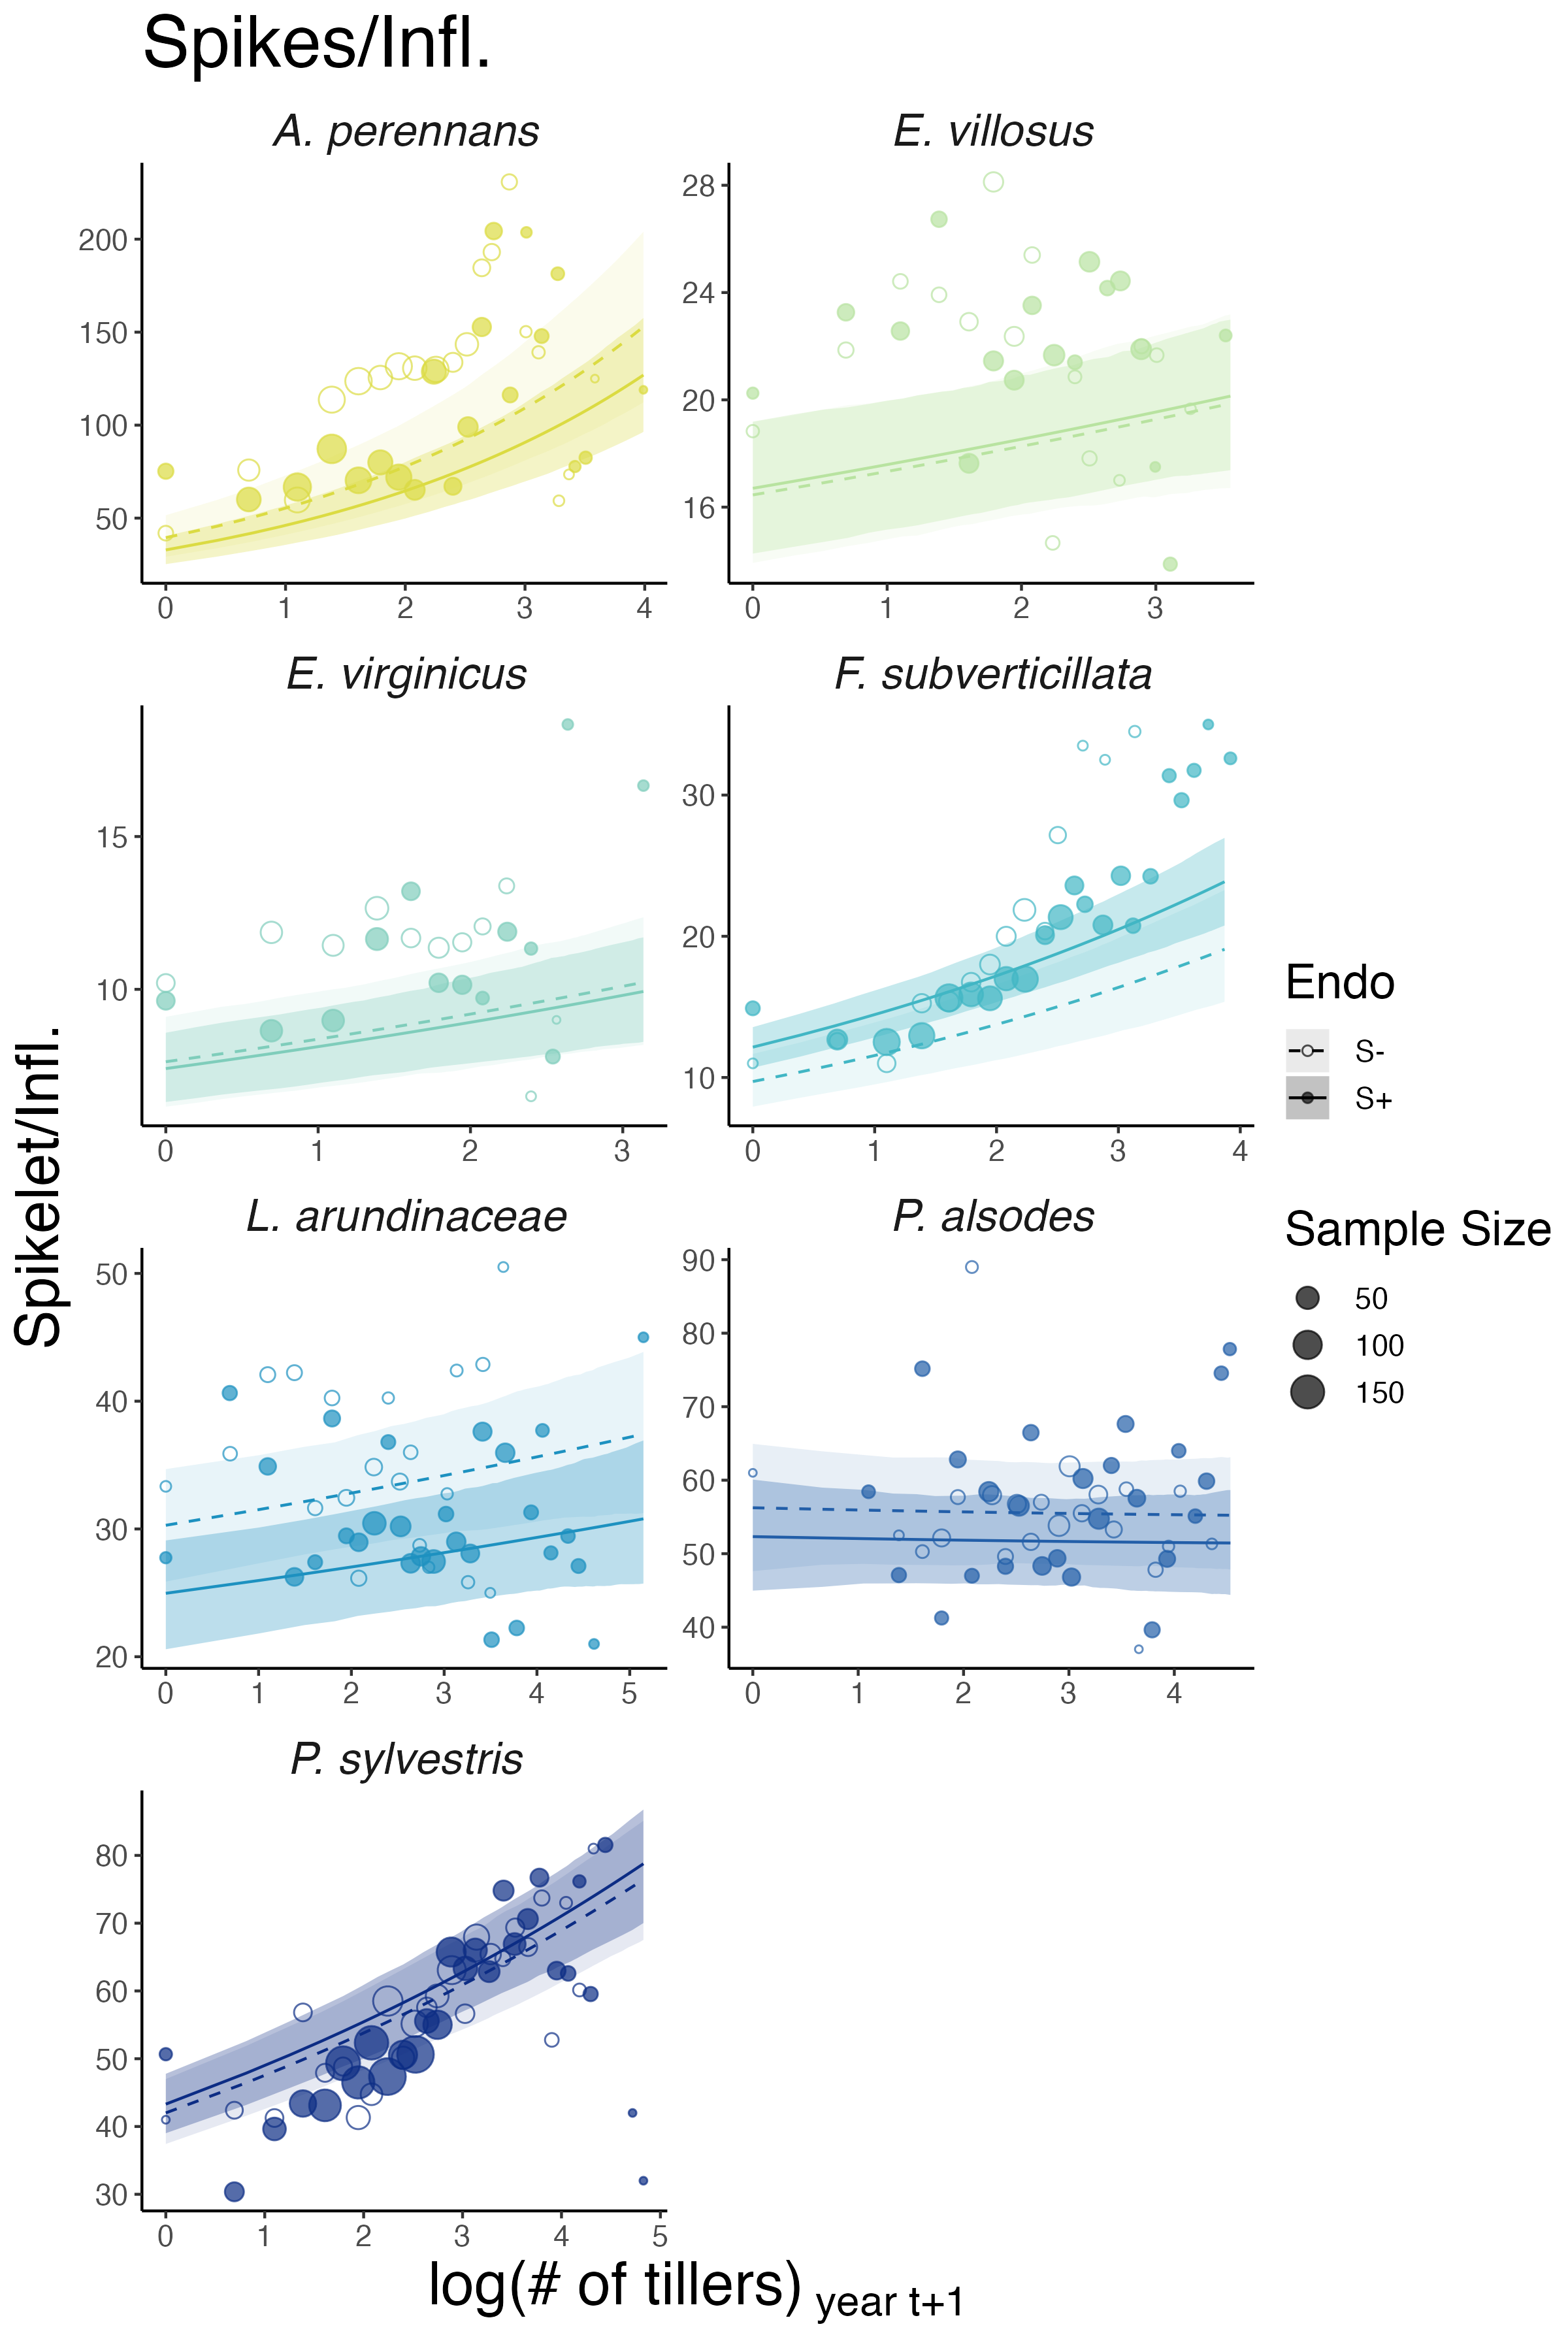
\includegraphics[width=.8\linewidth]{spike_meanplot.png}
\end{figure}
\noindent {\bf Fig. S5.} \textbf{Effect of endophyte symbiosis on the mean value of spikelet production.} Fitted curves represent the size-specific mean expected number of spikelets per inflorescence along with data binned by size shown as open circles with a dashed line for symbiont-free (S-) plants , while the solid line and filled circles represent symbiontic (S+) plants. 80\% credible intervals are shown with dark shading for  S+, or light shading for S-.
\newpage



\begin{figure}[H]
	\centering
	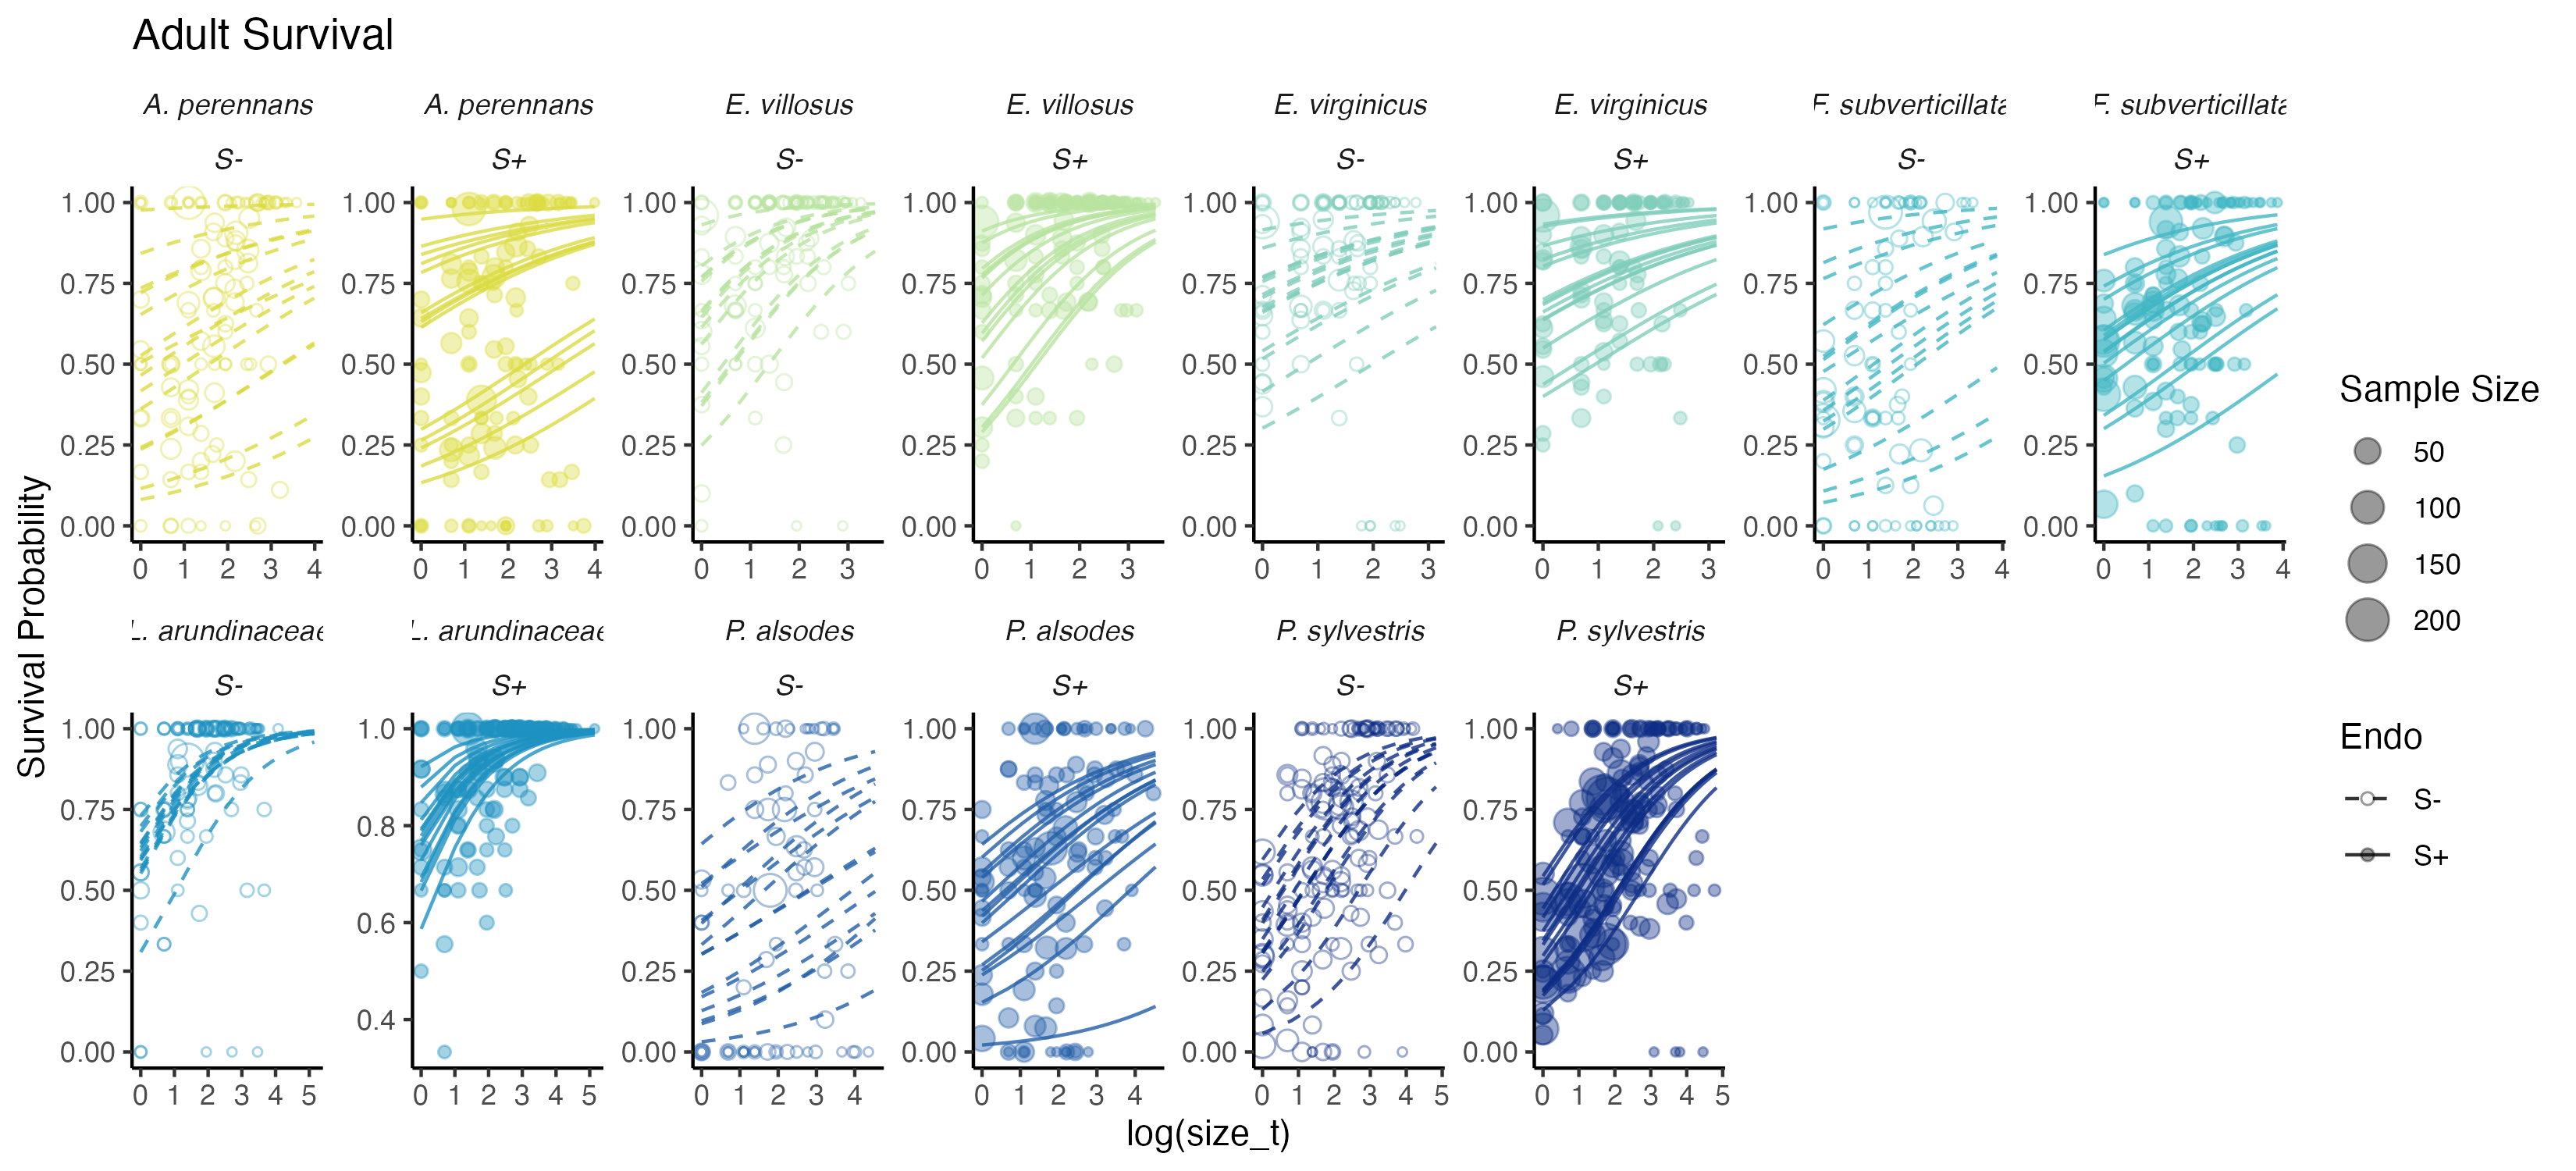
\includegraphics[width=.8\linewidth]{surv_yearplot.png}
\end{figure}
\noindent {\bf Fig. S6.} \textbf{Effect of endophyte symbiosis on yearly adult survival.} Fitted curves represent the size-specific annual survival probability along with data binned by size shown as open circles with a dashed line for symbiont-free (S-) plants , while the solid line and filled circles represent symbiontic (S+) plants. 
\begin{figure}[H]
	\centering
	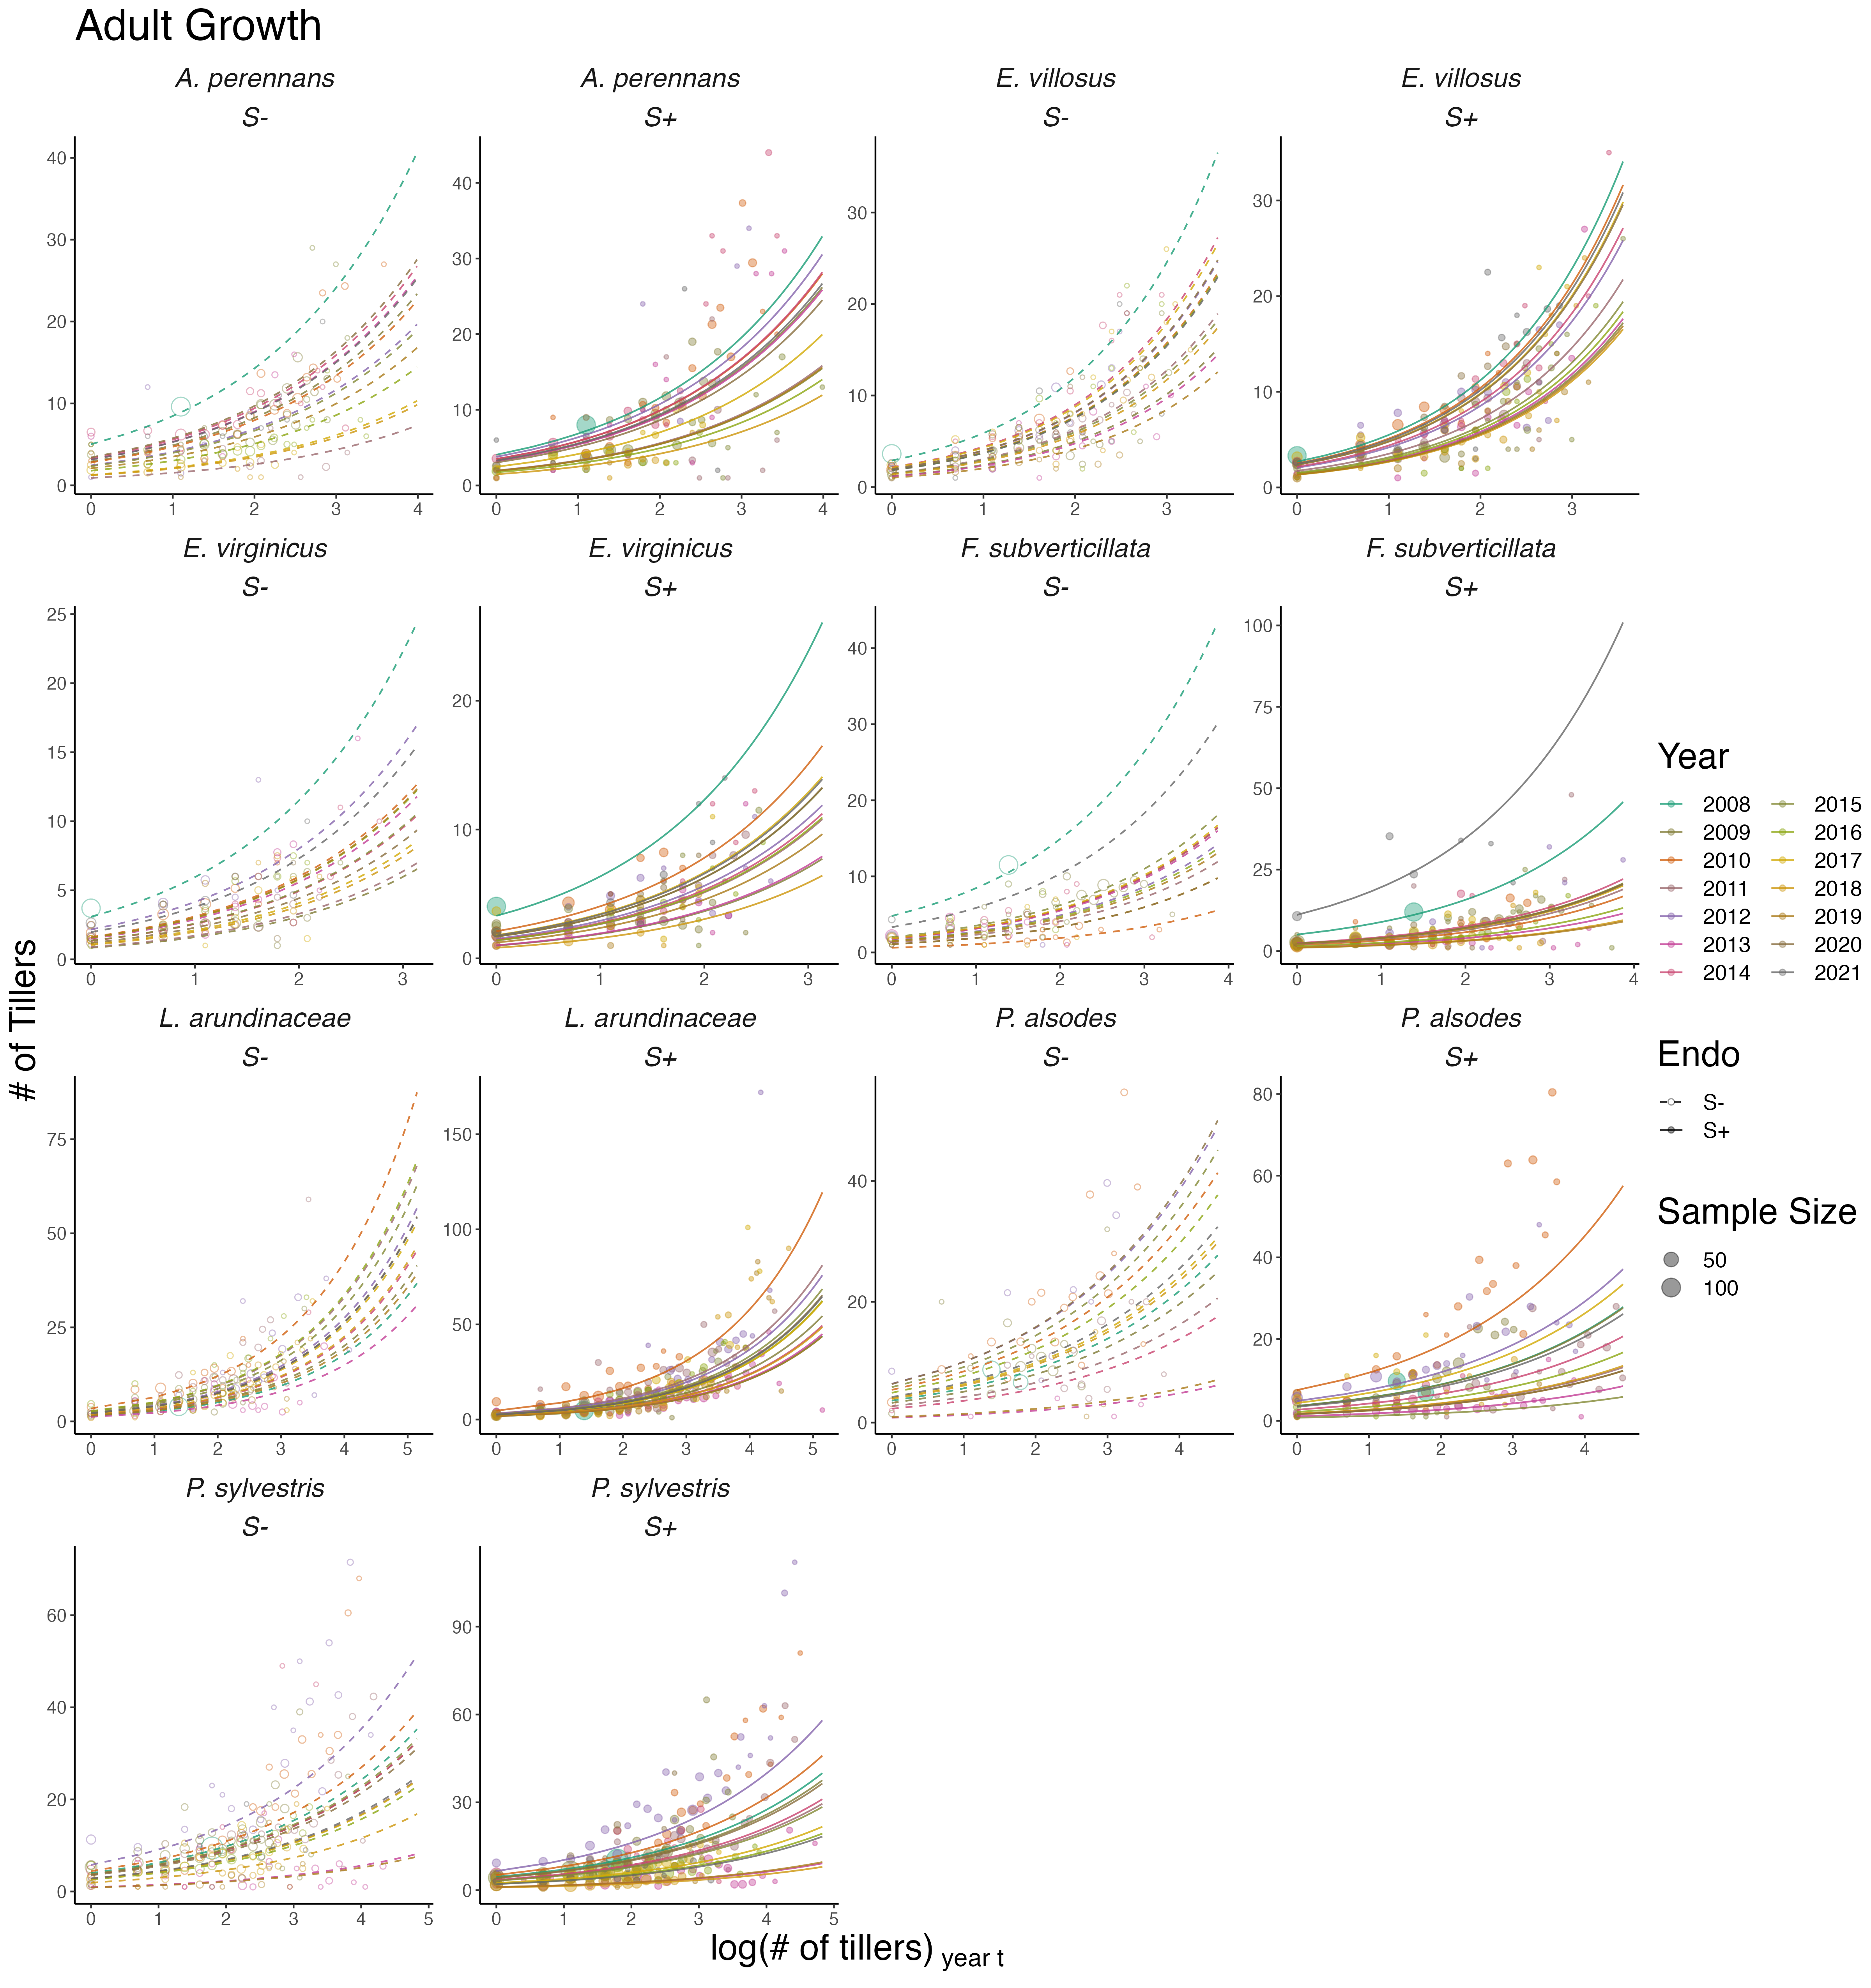
\includegraphics[width=.8\linewidth]{grow_yearplot.png}
\end{figure}
\noindent {\bf Fig. S7.} \textbf{Effect of endophyte symbiosis on yearly adult growth.} Fitted curves represent the size-specific annual expected plant size along with data binned by size shown as open circles with a dashed line for symbiont-free (S-) plants , while the solid line and filled circles represent symbiontic (S+) plants. 
\newpage

\begin{figure}[H]
	\centering
	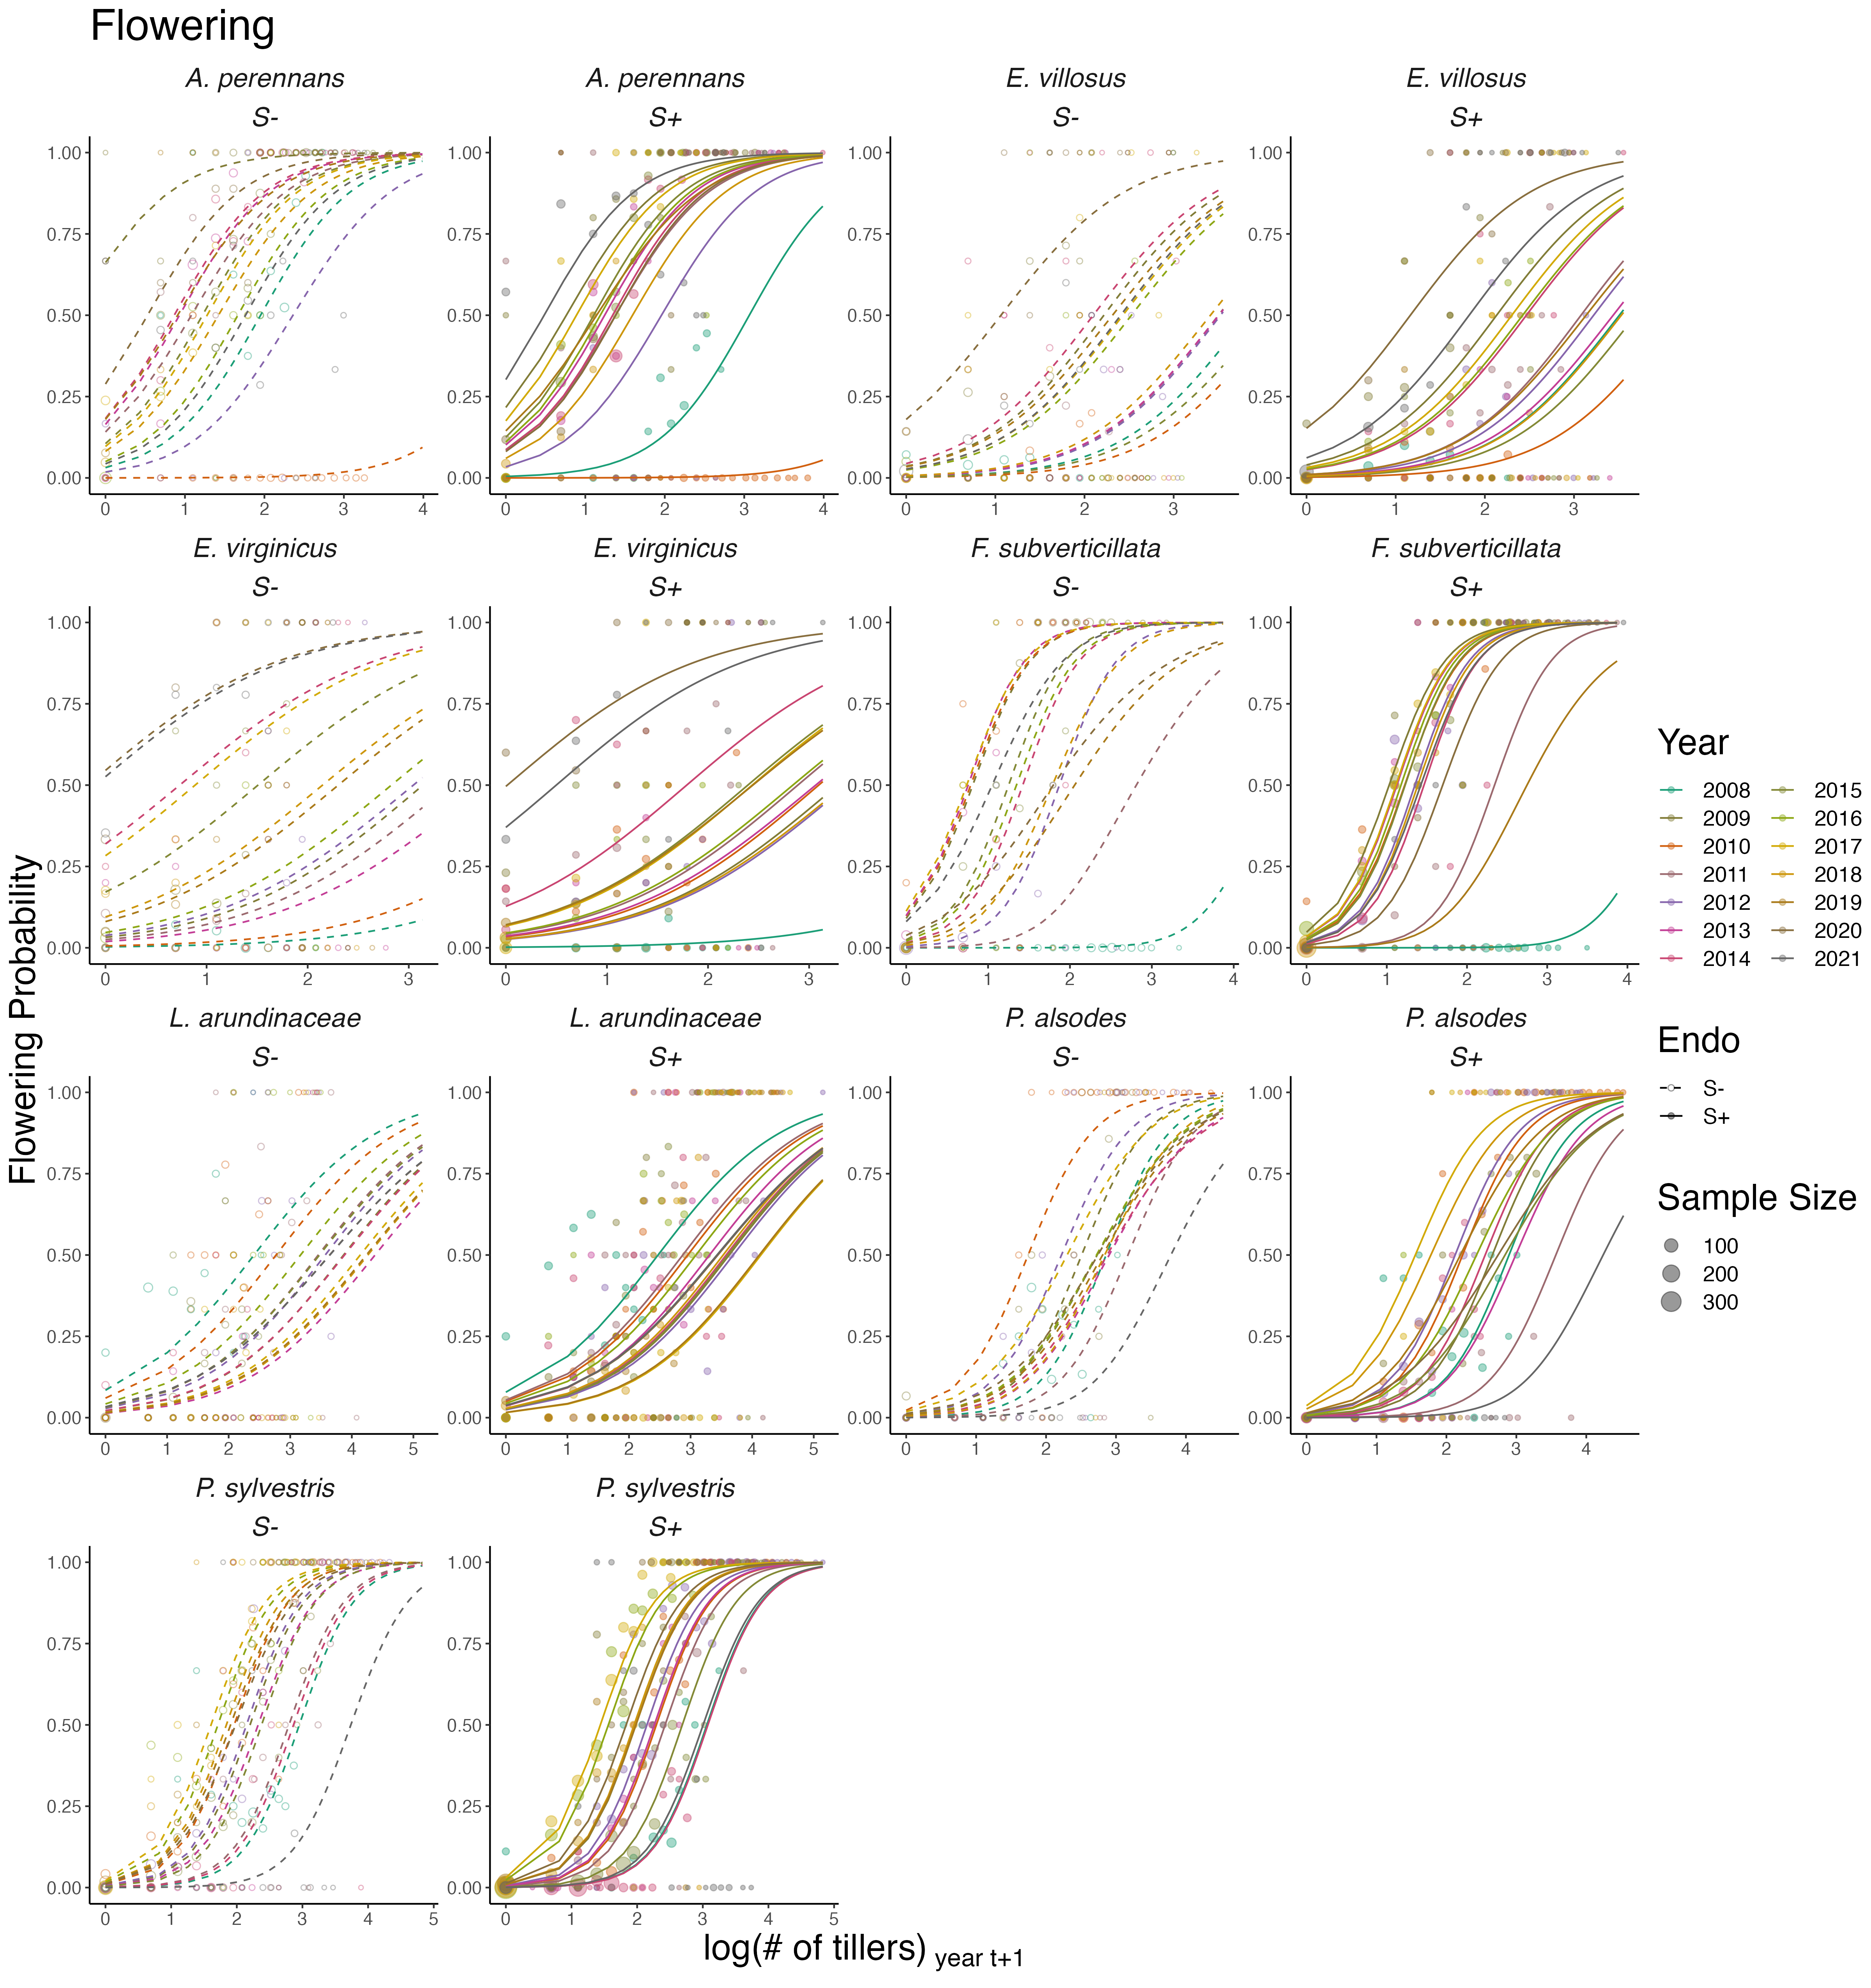
\includegraphics[width=.8\linewidth]{flw_yearplot.png}
\end{figure}
\noindent {\bf Fig. S8.} \textbf{Effect of endophyte symbiosis on yearly flowering} Fitted curves represent the size-specific annual flowering probability along with data binned by size shown as open circles with a dashed line for symbiont-free (S-) plants , while the solid line and filled circles represent symbiontic (S+) plants.
\begin{figure}[H]
	\centering
	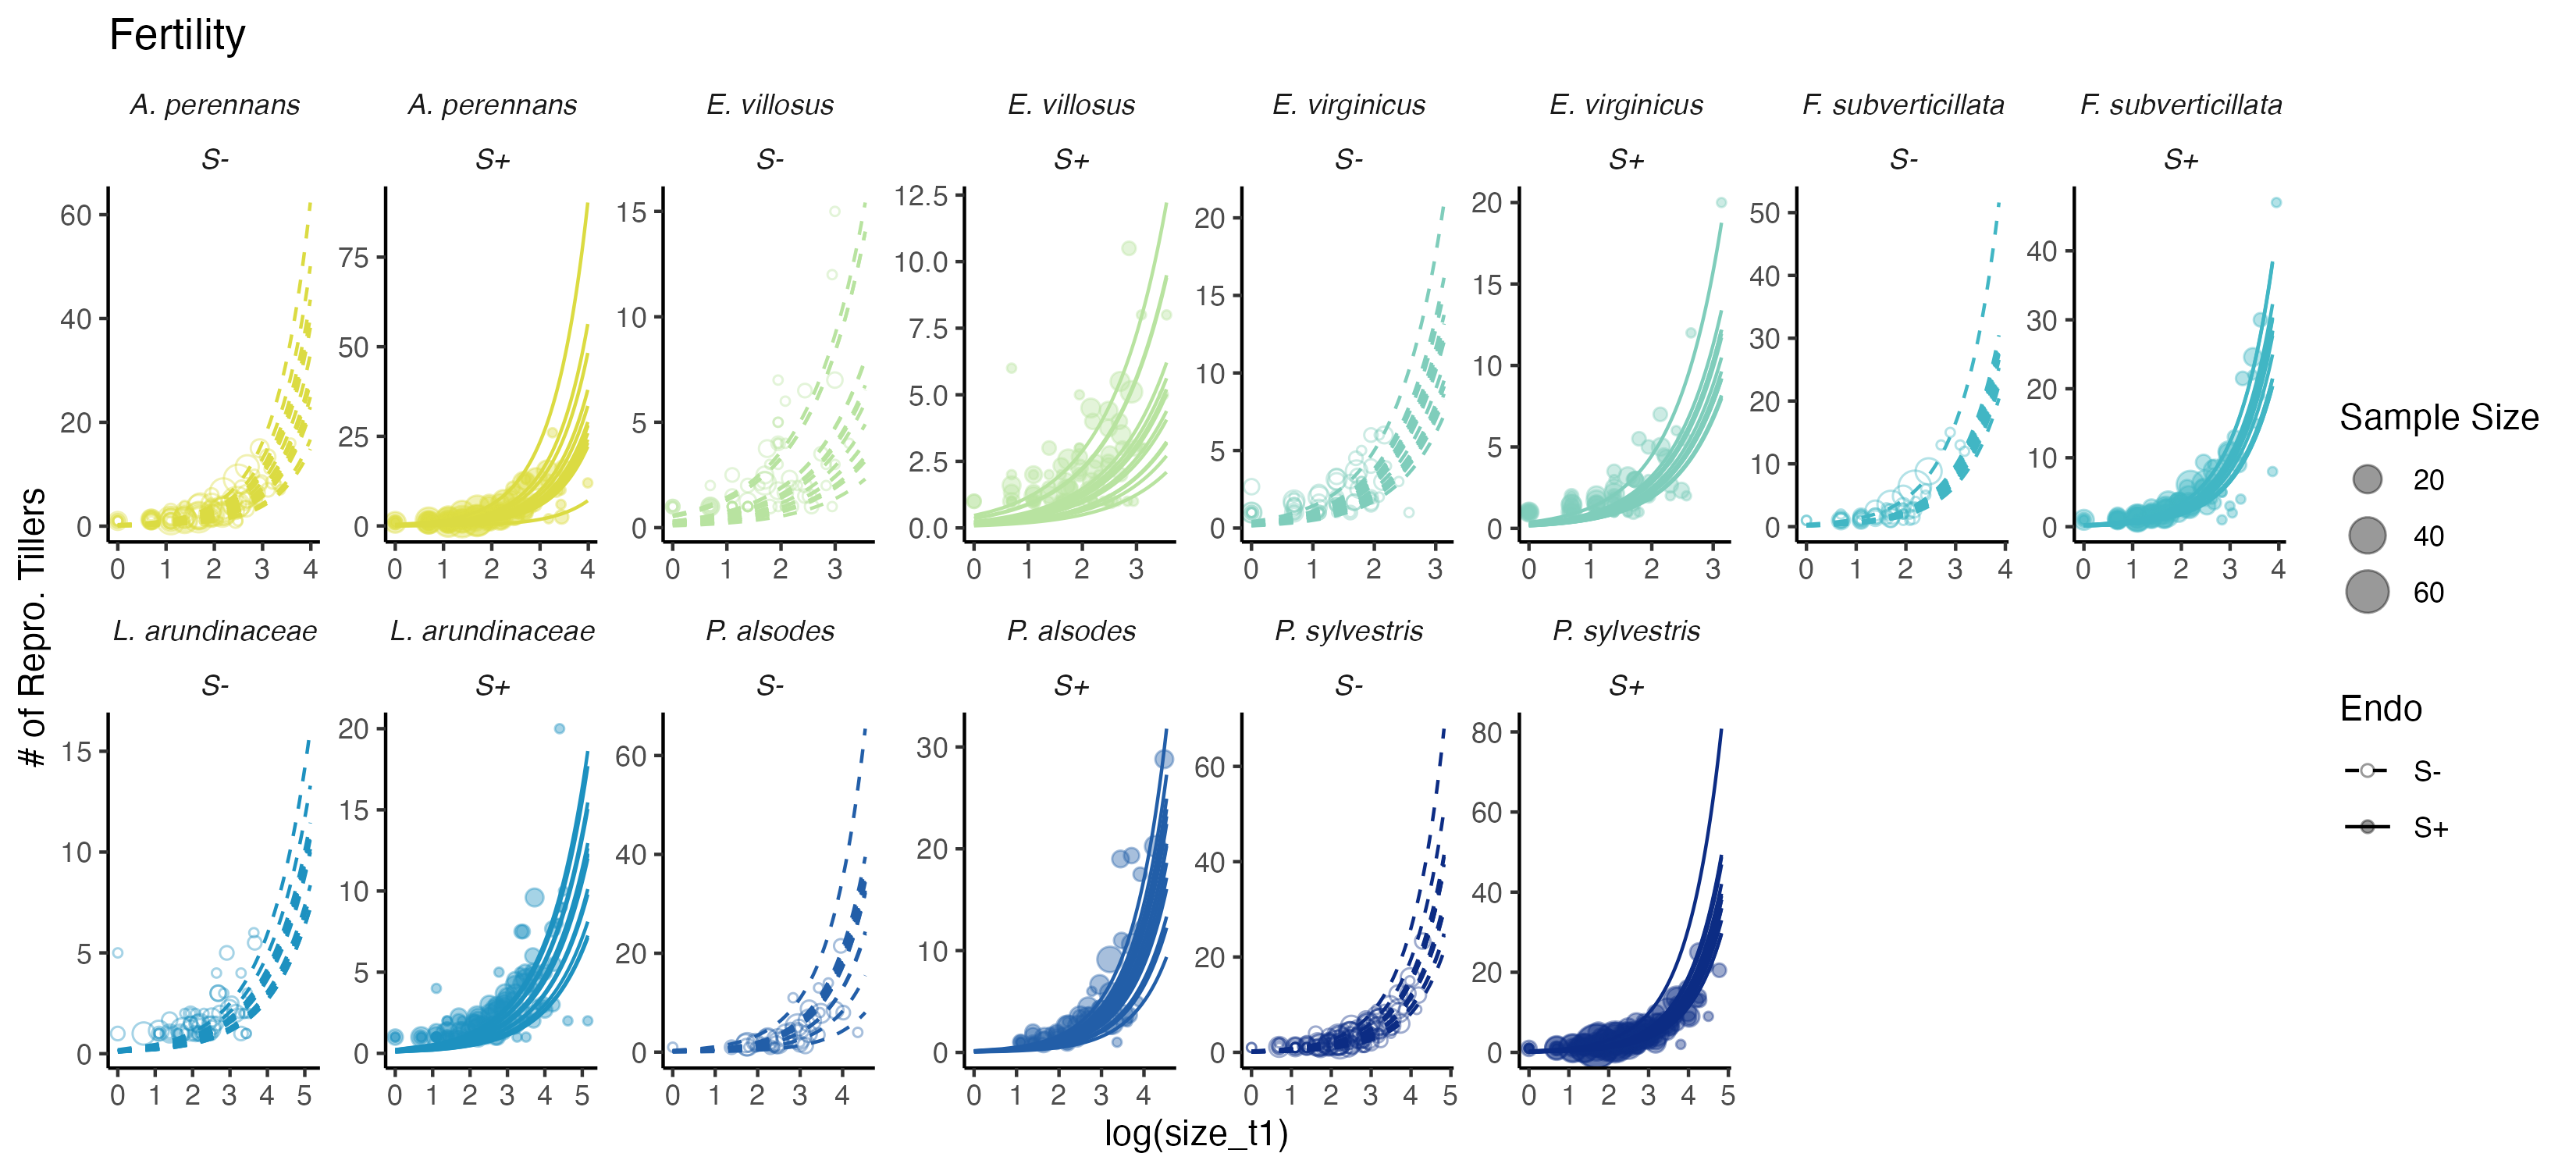
\includegraphics[width=.8\linewidth]{fert_yearplot.png}
\end{figure}
\noindent {\bf Fig. S9.} \textbf{Effect of endophyte symbiosis on yearly fertility.} Fitted curves represent the size-specific annual expected number of flowering tillers along with data binned by size shown as open circles with a dashed line for symbiont-free (S-) plants , while the solid line and filled circles represent symbiontic (S+) plants. 
\newpage
\begin{figure}[H]
	\centering
	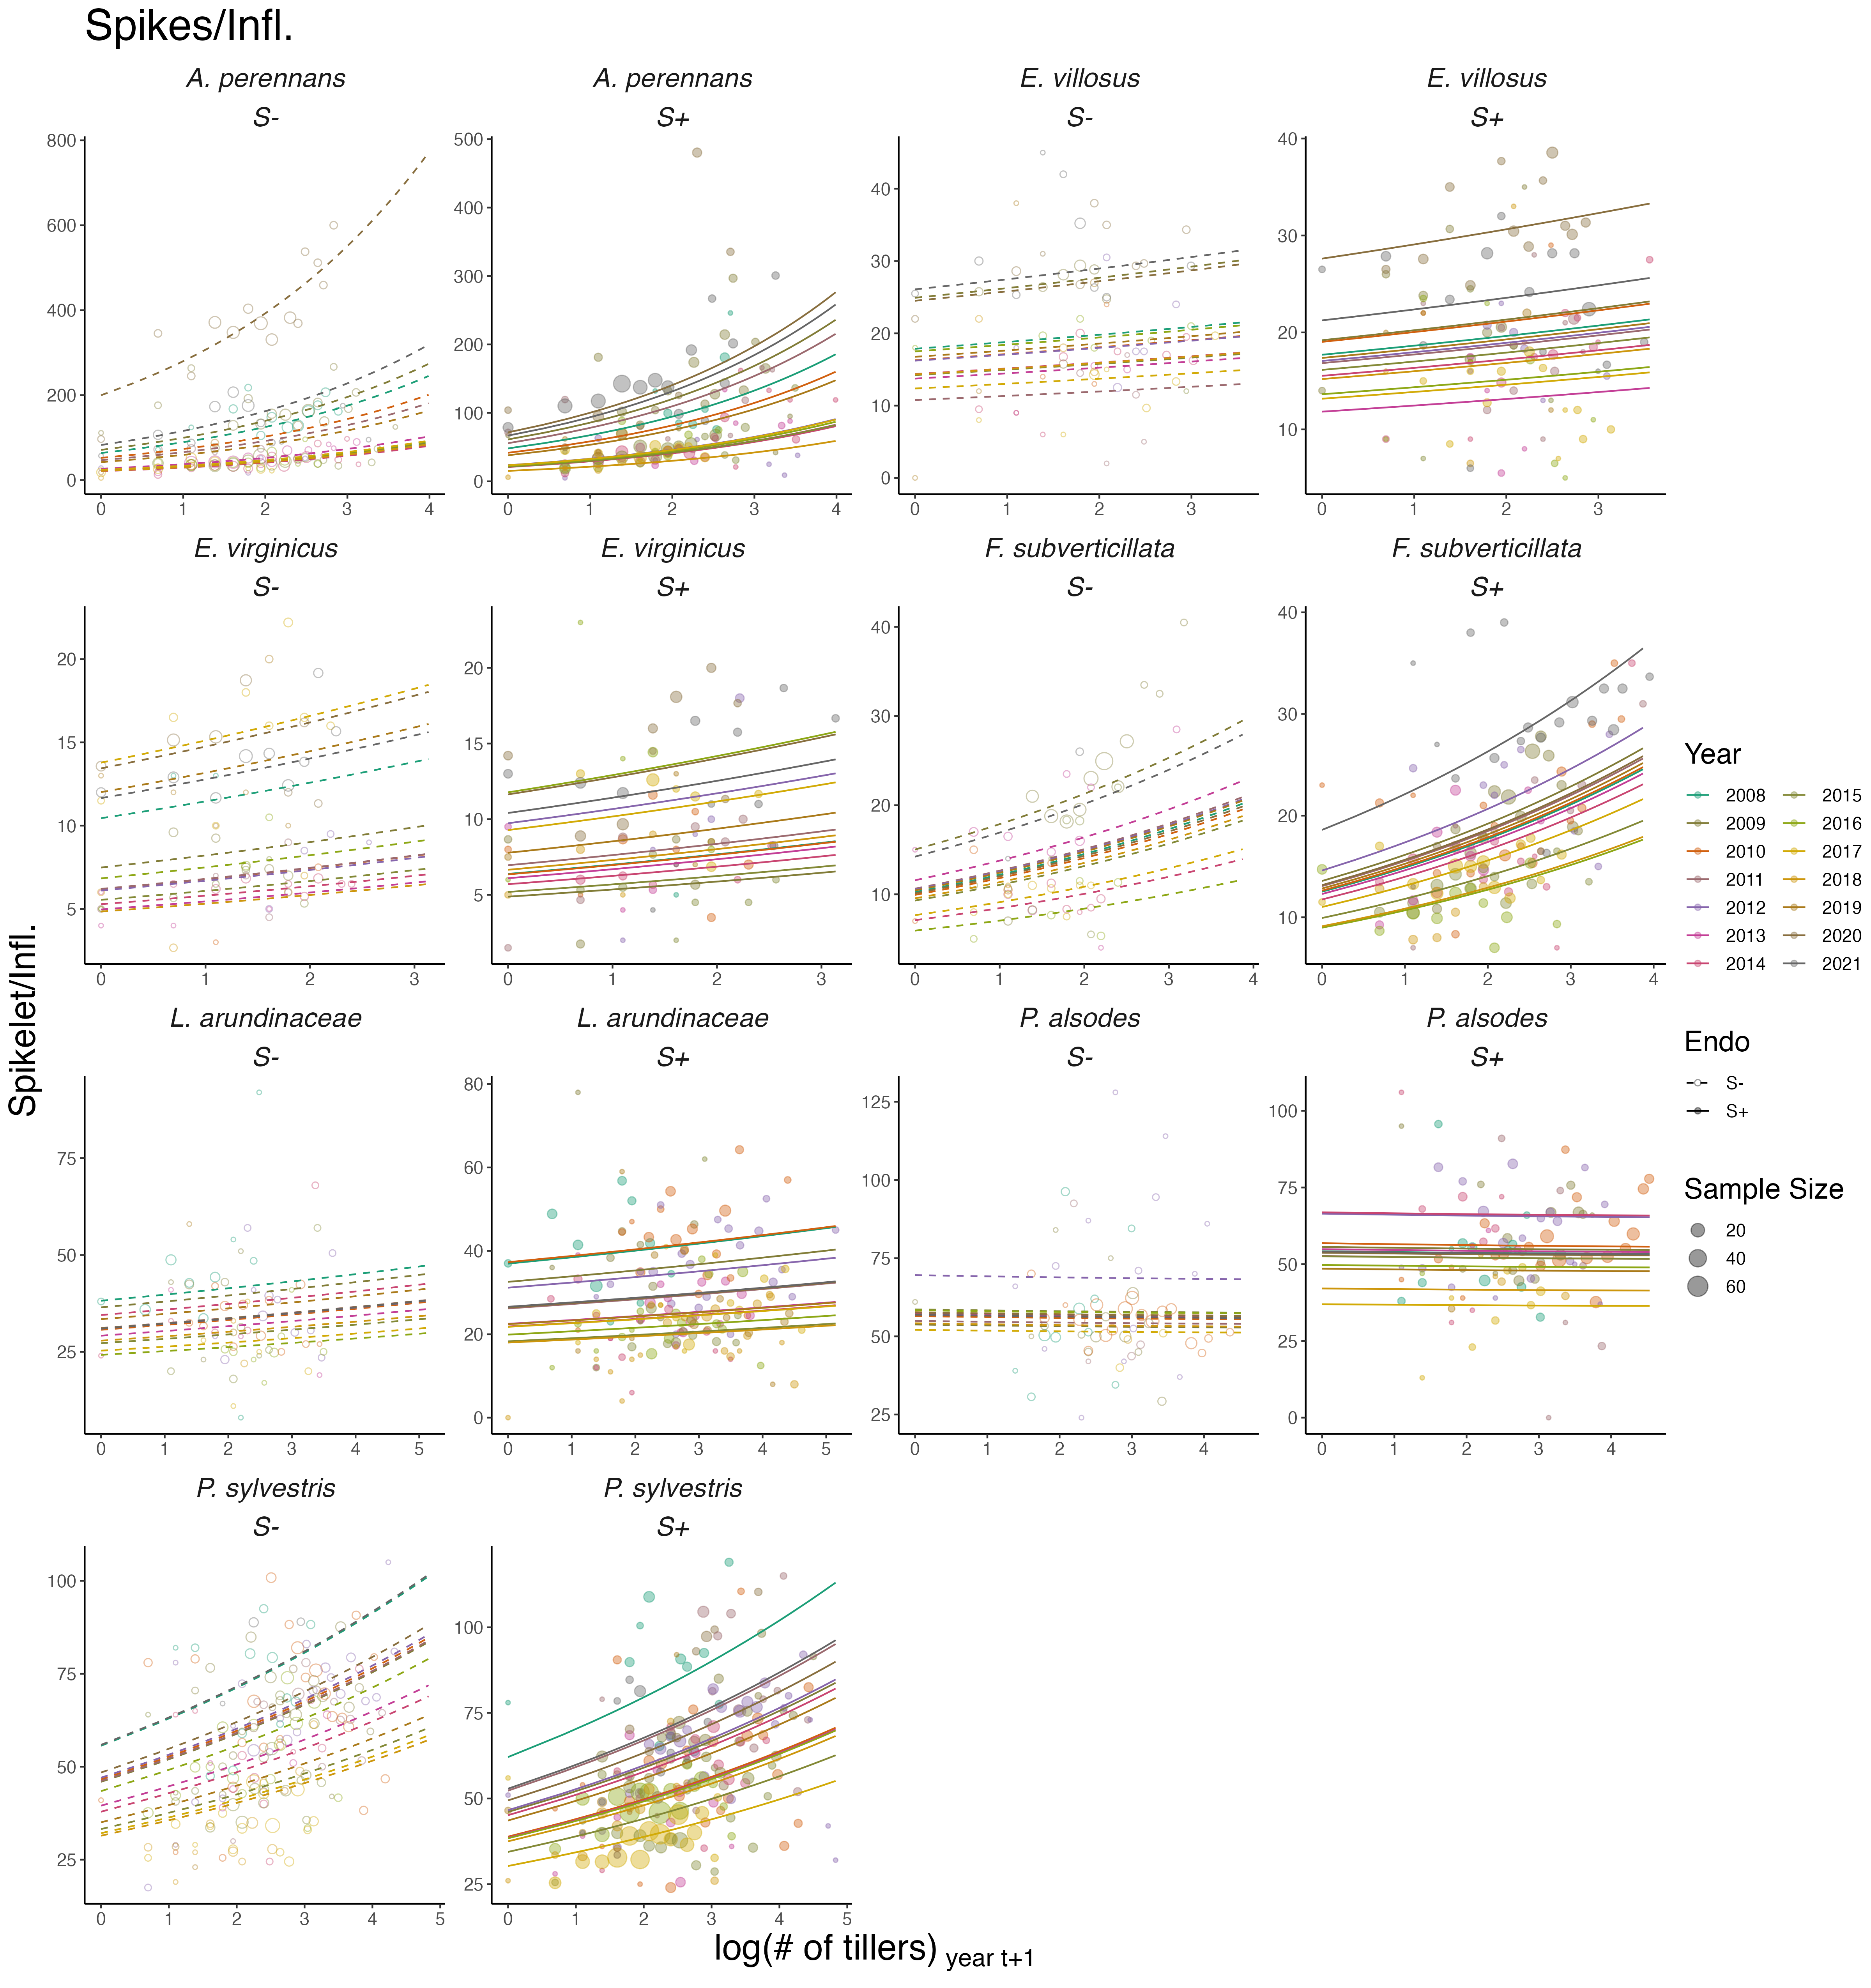
\includegraphics[width=.8\linewidth]{spike_yearplot.png}
\end{figure}
\noindent {\bf Fig. S10.} \textbf{Effect of endophyte symbiosis on yearly spikelet production.} Fitted curves represent the size-specific annual expected number of spikelets per inflorescence along with data binned by size shown as open circles with a dashed line for symbiont-free (S-) plants , while the solid line and filled circles represent symbiontic (S+) plants.
\newpage


\begin{figure}[H]
	\centering
	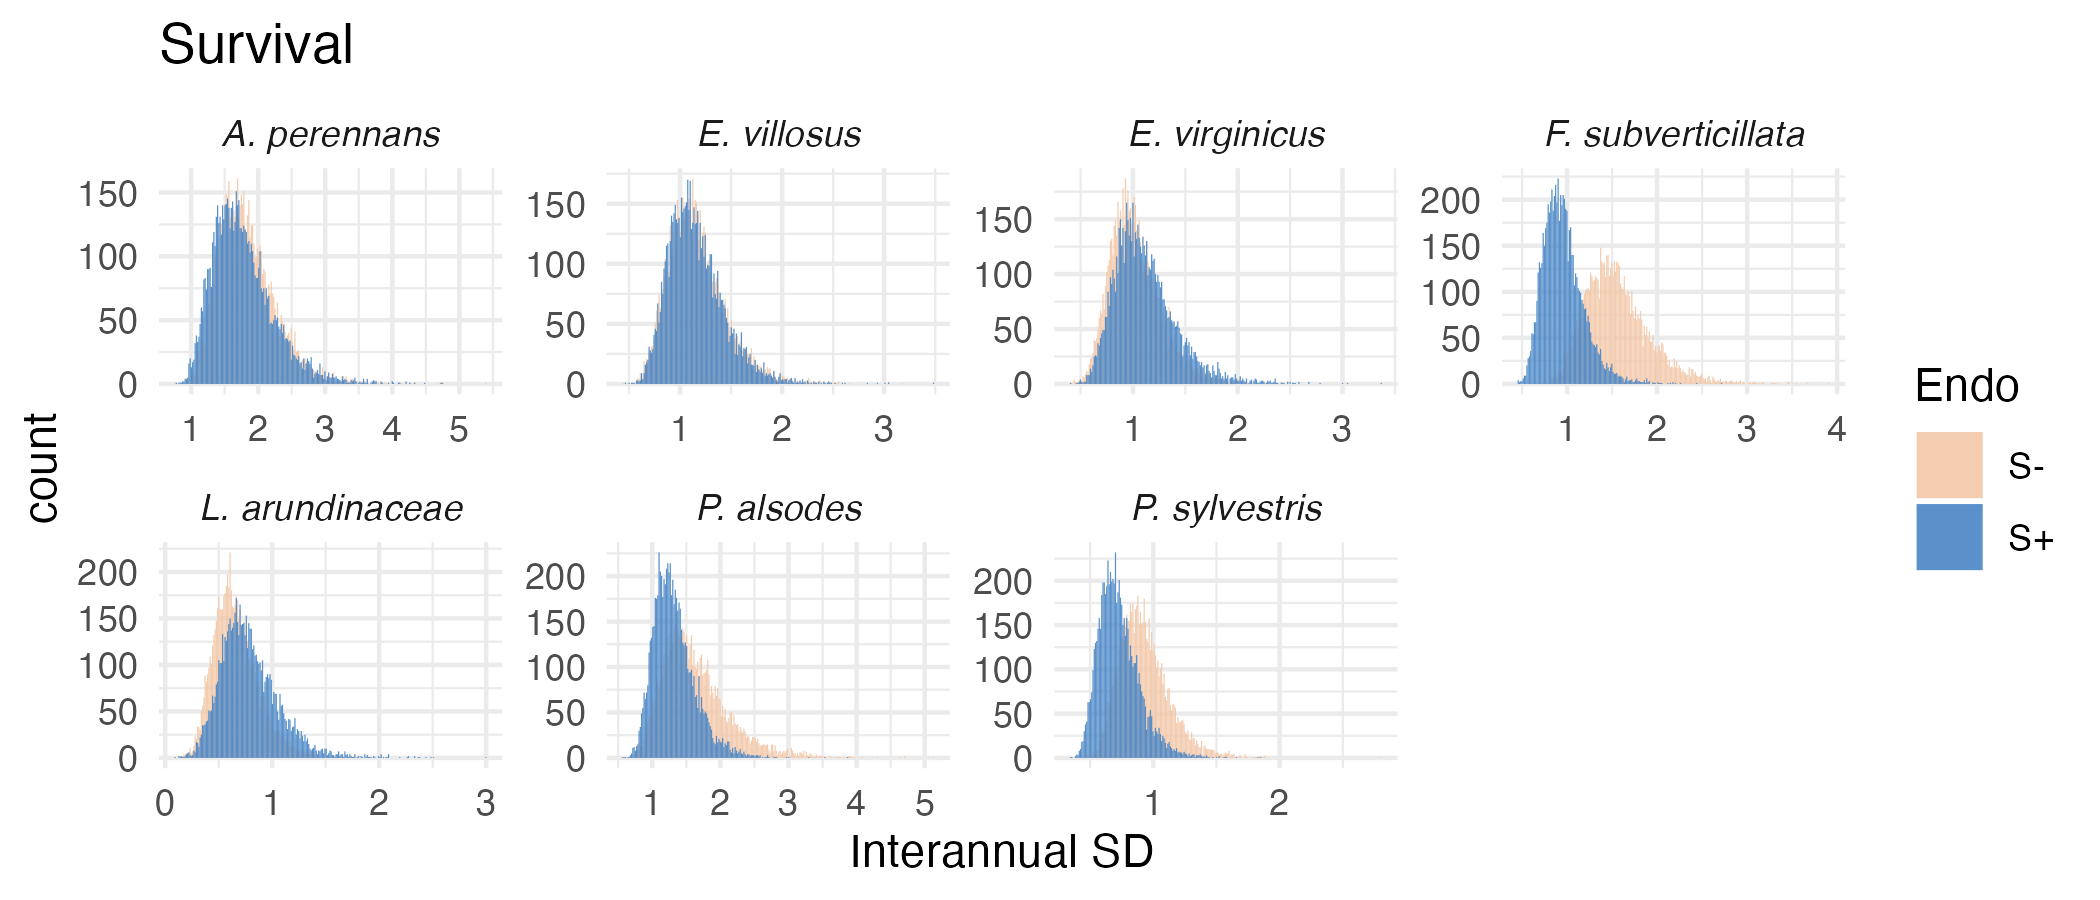
\includegraphics[width=.9\linewidth]{surv_sigmayear_hist.png}
\end{figure}
\noindent {\bf Fig. S11.} \textbf{Posterior distributions of the standard deviations of interannual year effects for survival.} Histograms include 7500 post-warmup MCMC samples for symbiotic (S+; blue) and symbiont-free (S-; tan) plants from fitted vital rate model.


\begin{figure}[H]
	\centering
	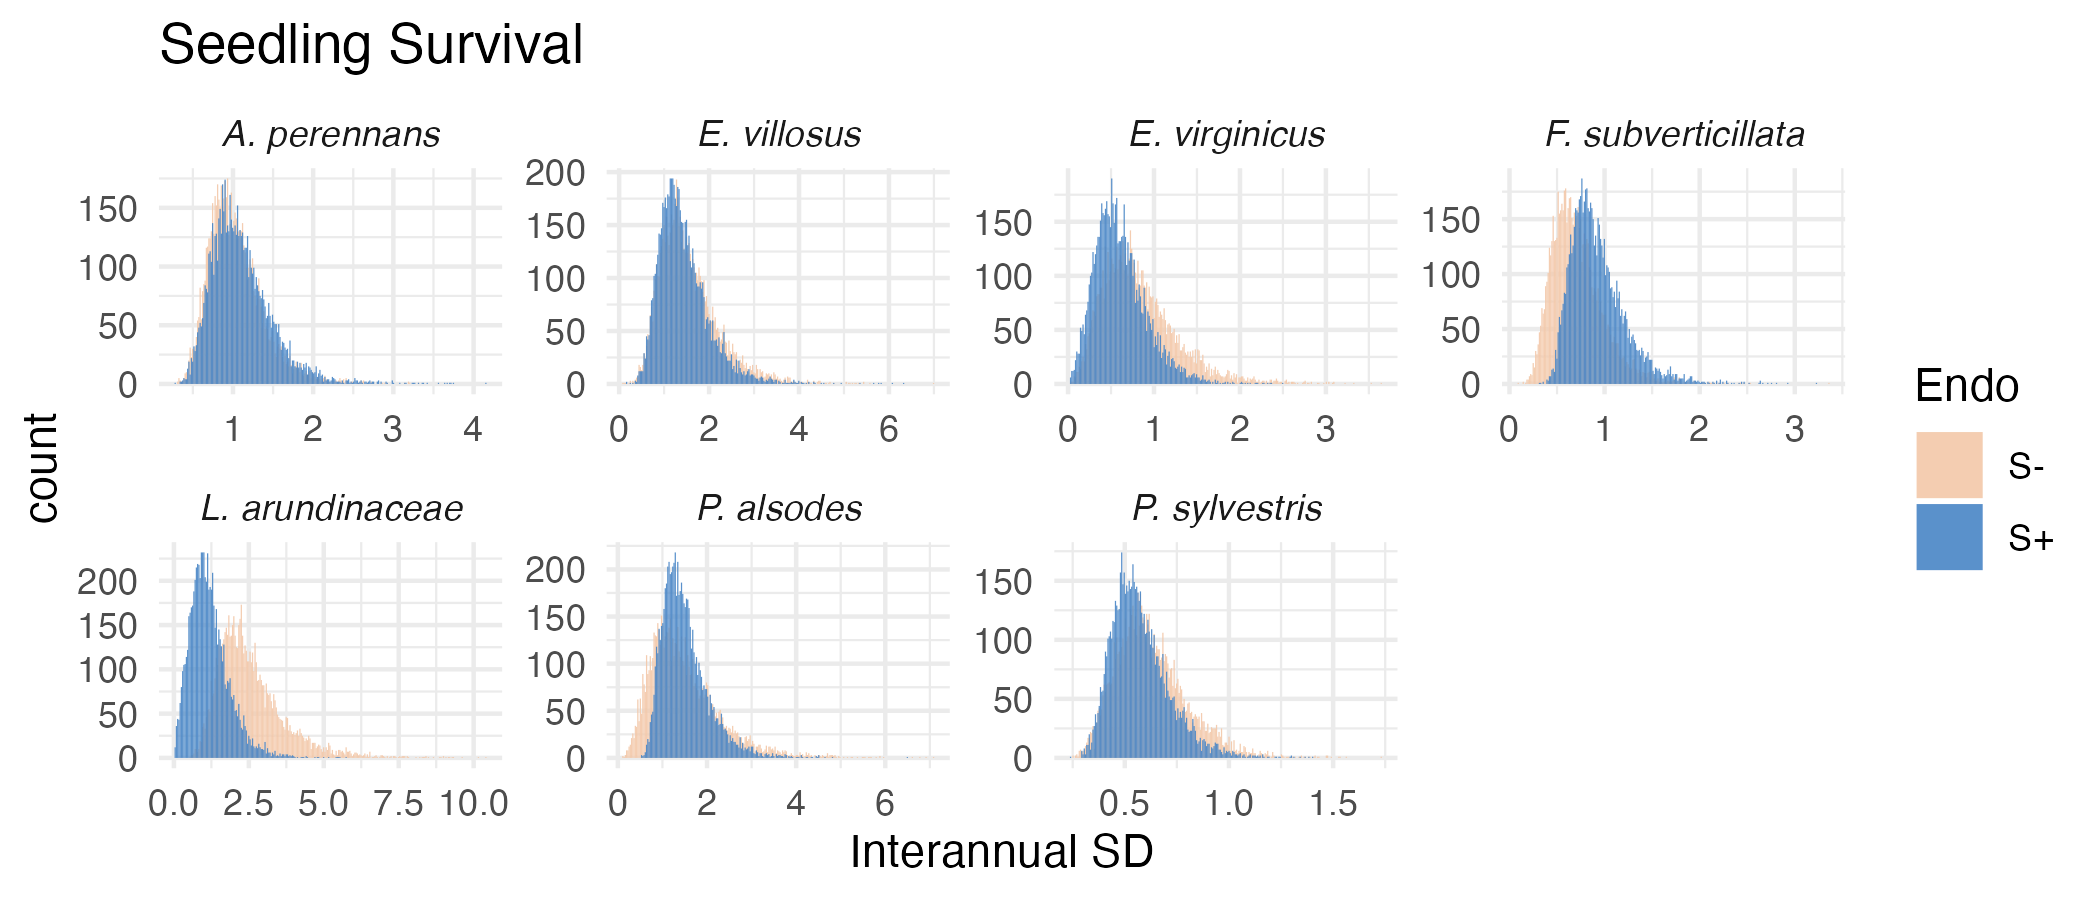
\includegraphics[width=.9\linewidth]{seedsurv_sigmayear_hist.png}
\end{figure}
\noindent {\bf Fig. S12.} \textbf{Posterior distributions of the standard deviations of interannual year effects for seedling survival.} Histograms include 7500 post-warmup MCMC samples for symbiotic (S+; blue) and symbiont-free (S-; tan) plants from fitted vital rate model.
\newpage

\begin{figure}[H]
	\centering
	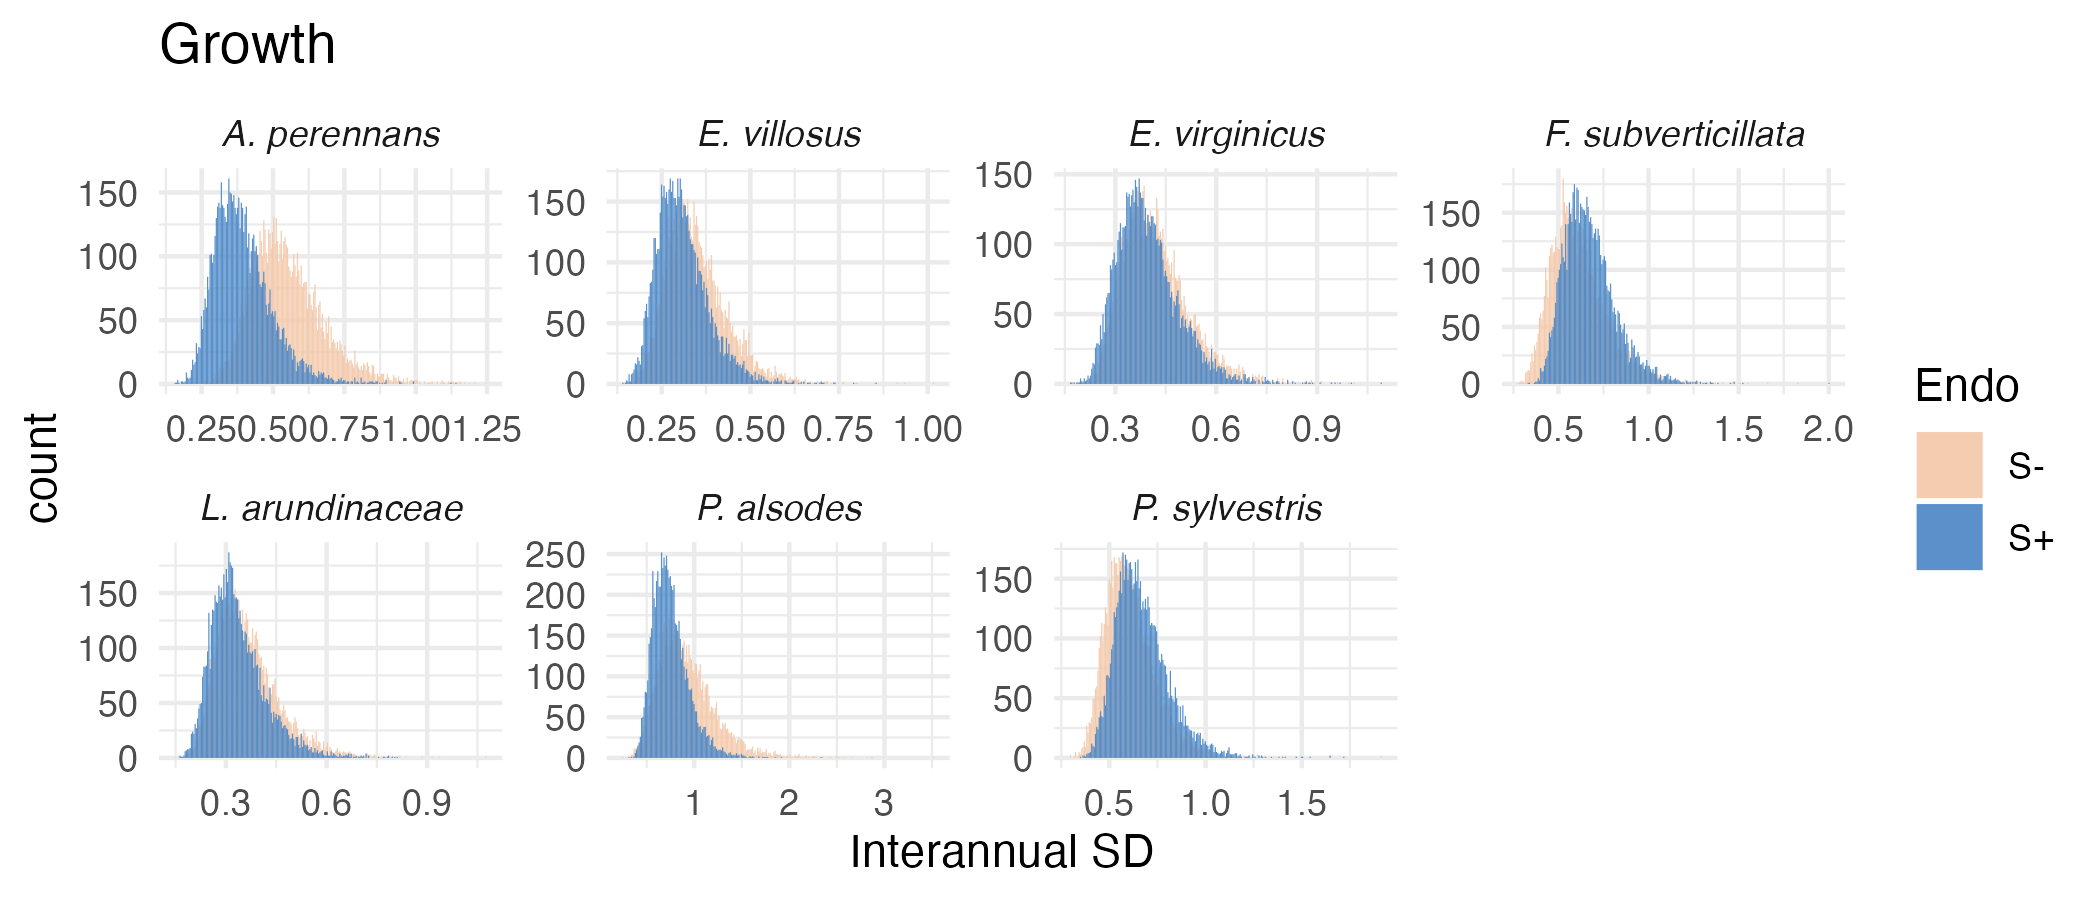
\includegraphics[width=.9\linewidth]{grow_sigmayear_hist.png}
\end{figure}
\noindent {\bf Fig. S13.} \textbf{Posterior distributions of the standard deviations of interannual year effects for growth.} Histograms include 7500 post-warmup MCMC samples for symbiotic (S+; blue) and symbiont-free (S-; tan) plants from fitted vital rate model.

\begin{figure}[H]
	\centering
	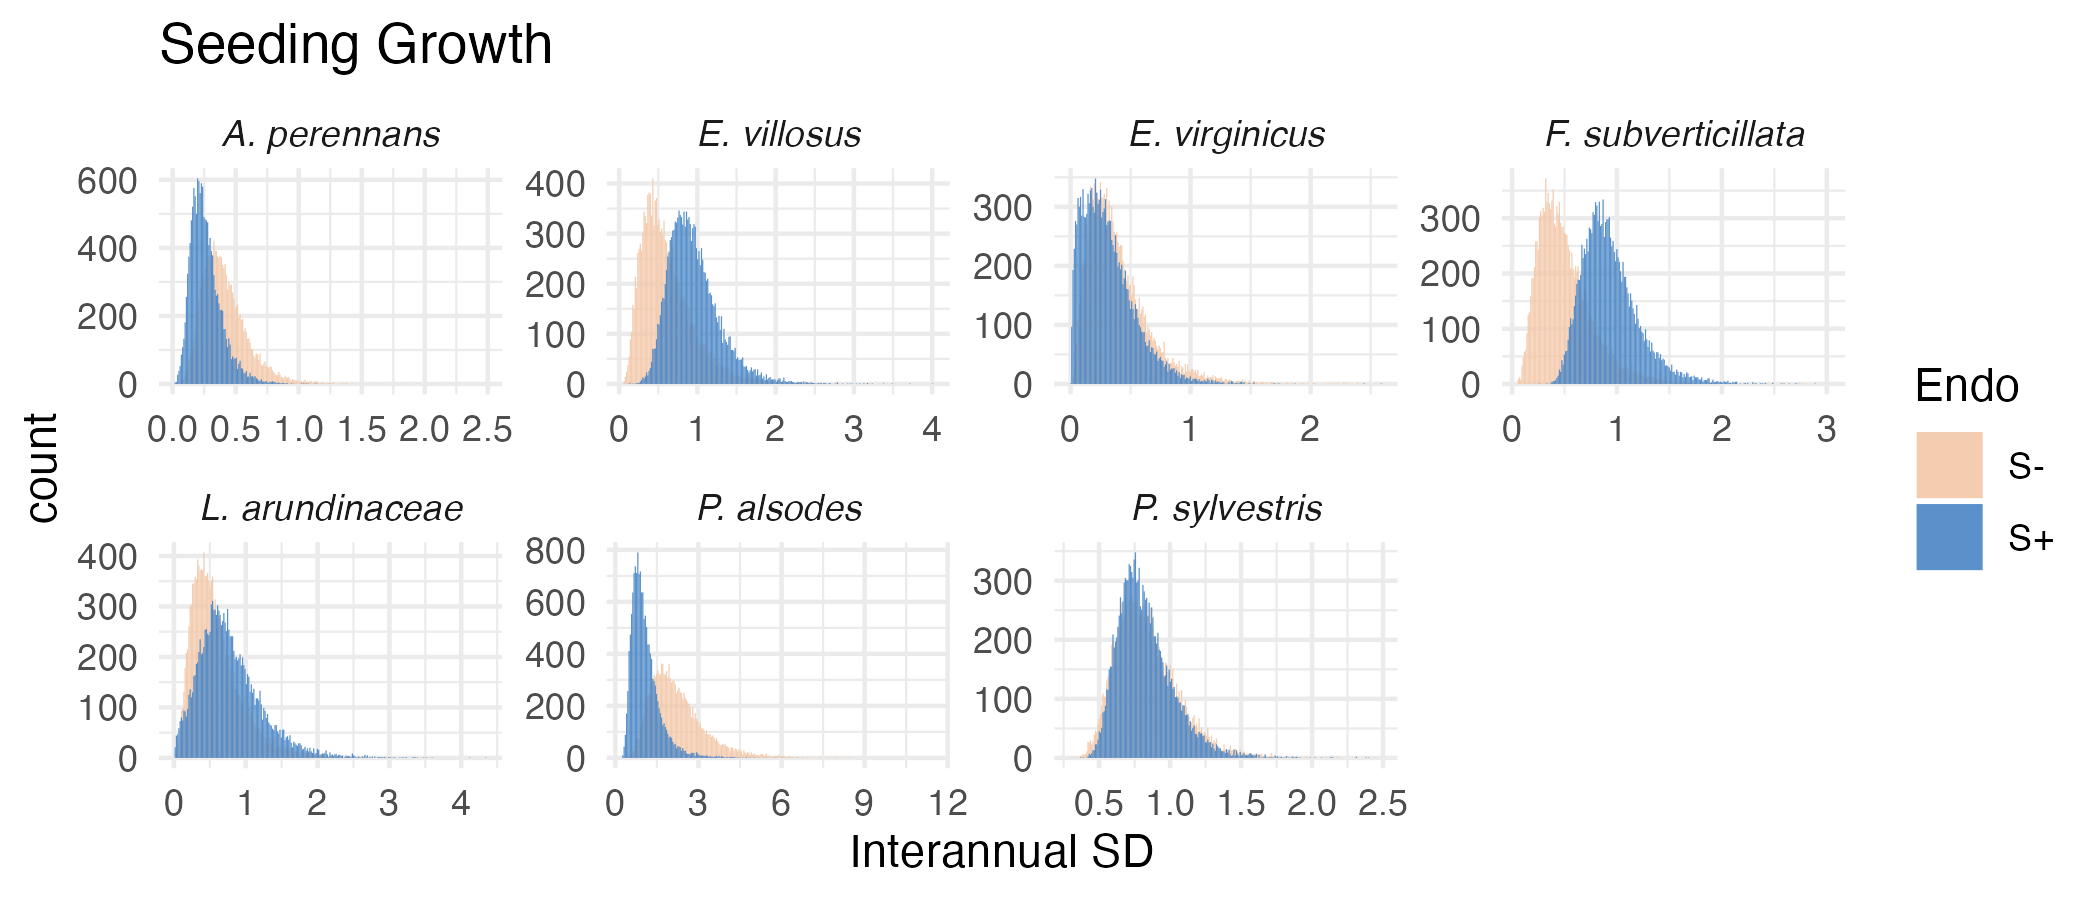
\includegraphics[width=.9\linewidth]{seedgrow_sigmayear_hist.png}
\end{figure}
\noindent {\bf Fig. S14.} \textbf{Posterior distributions of the standard deviations of interannual year effects for seedling growth.} Histograms include 7500 post-warmup MCMC samples for symbiotic (S+; blue) and symbiont-free (S-; tan) plants from fitted vital rate model.
\newpage

\begin{figure}[H]
	\centering
	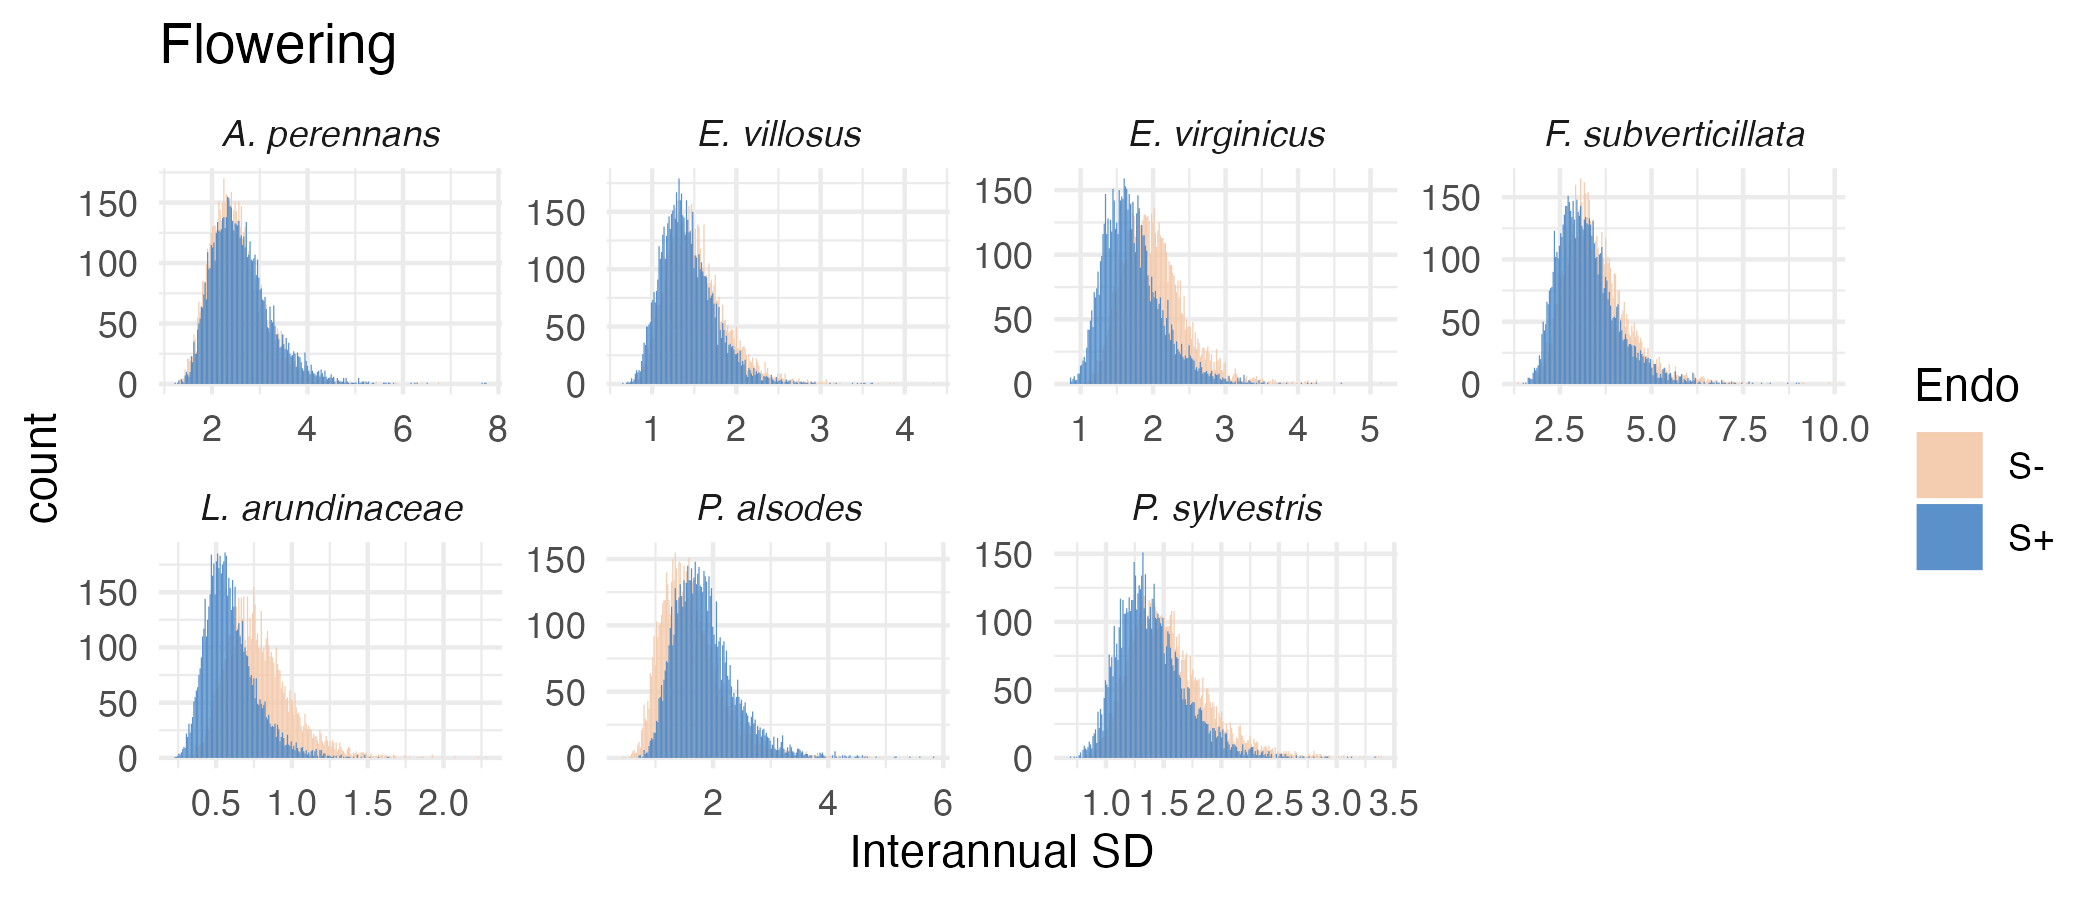
\includegraphics[width=.9\linewidth]{flow_sigmayear_hist.png}
\end{figure}
\noindent {\bf Fig. S15.} \textbf{Posterior distributions of the standard deviations of interannual year effects for flowering probability.} Histograms include 7500 post-warmup MCMC samples for symbiotic (S+; blue) and symbiont-free (S-; tan) plants from fitted vital rate model.


\begin{figure}[H]
	\centering
	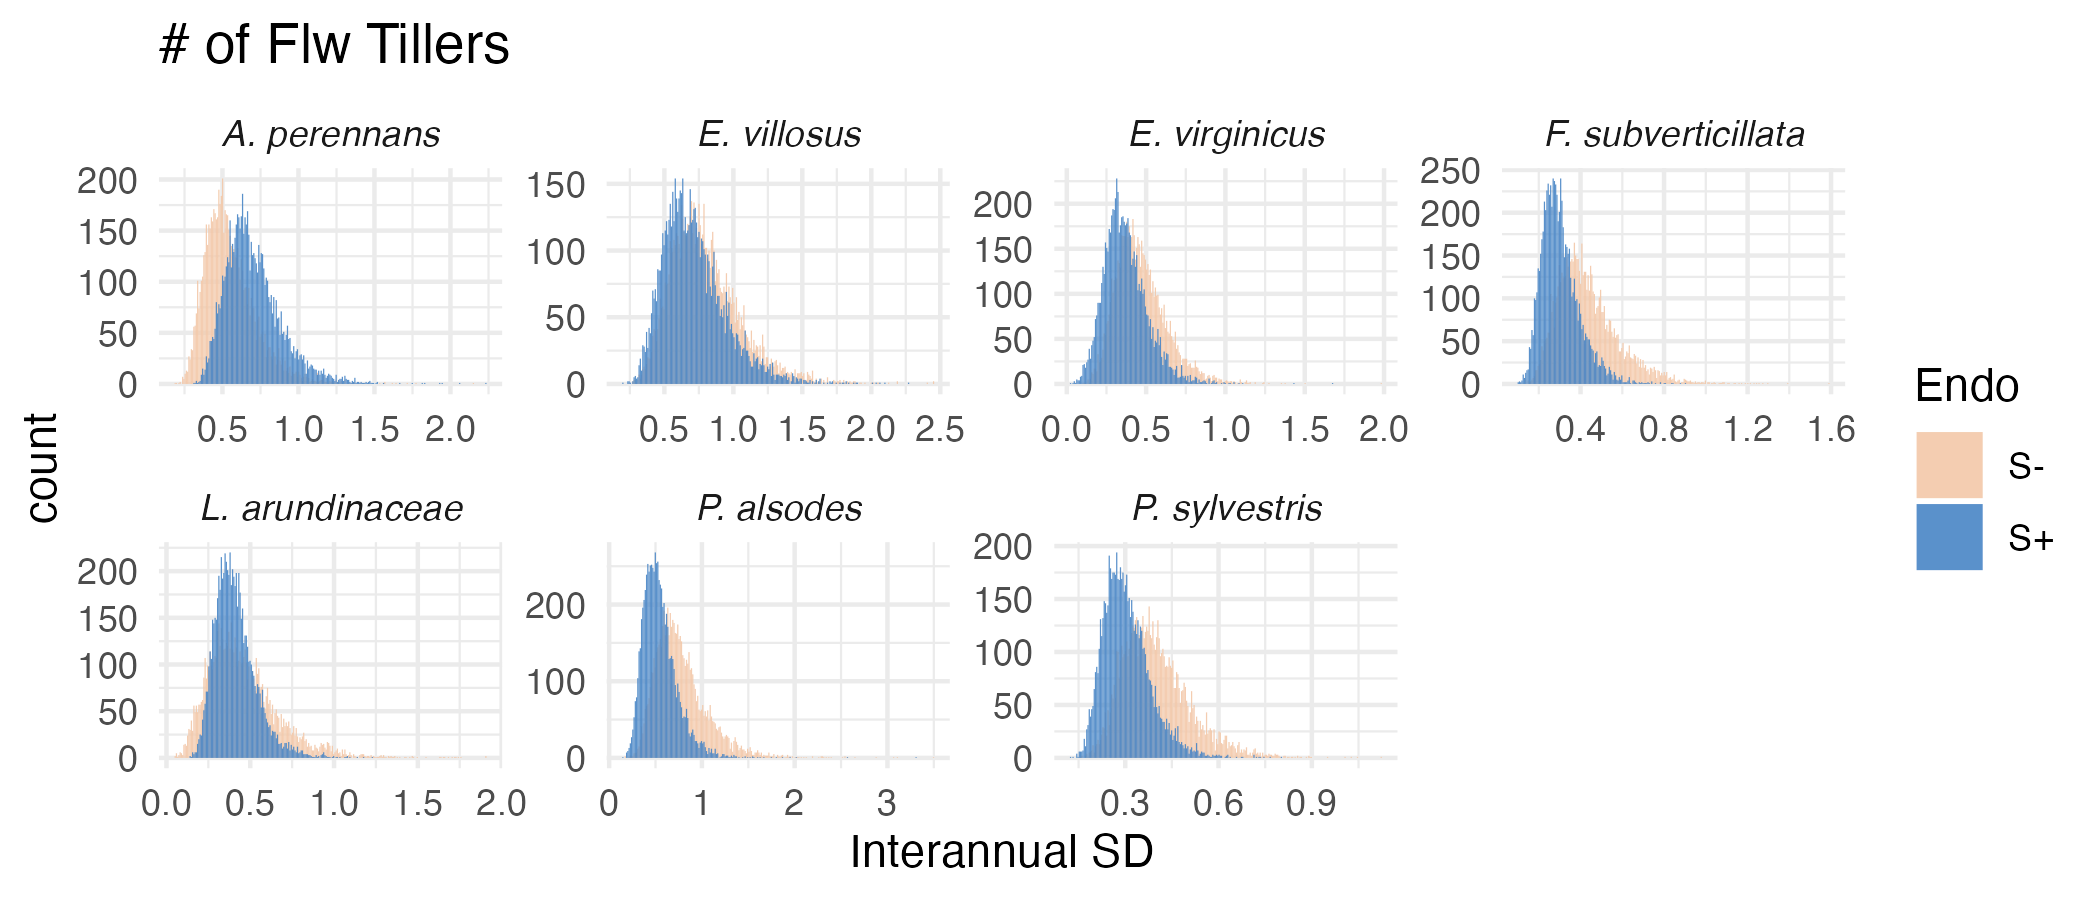
\includegraphics[width=.9\linewidth]{fert_sigmayear_hist.png}
\end{figure}
\noindent {\bf Fig. S16.} \textbf{Posterior distributions of the standard deviations of interannual year effects for fertility (no. of flowering tillers).} Histograms include 7500 post-warmup MCMC samples for symbiotic (S+; blue) and symbiont-free (S-; tan) plants from fitted vital rate model.
\newpage

\begin{figure}[H]
	\centering
	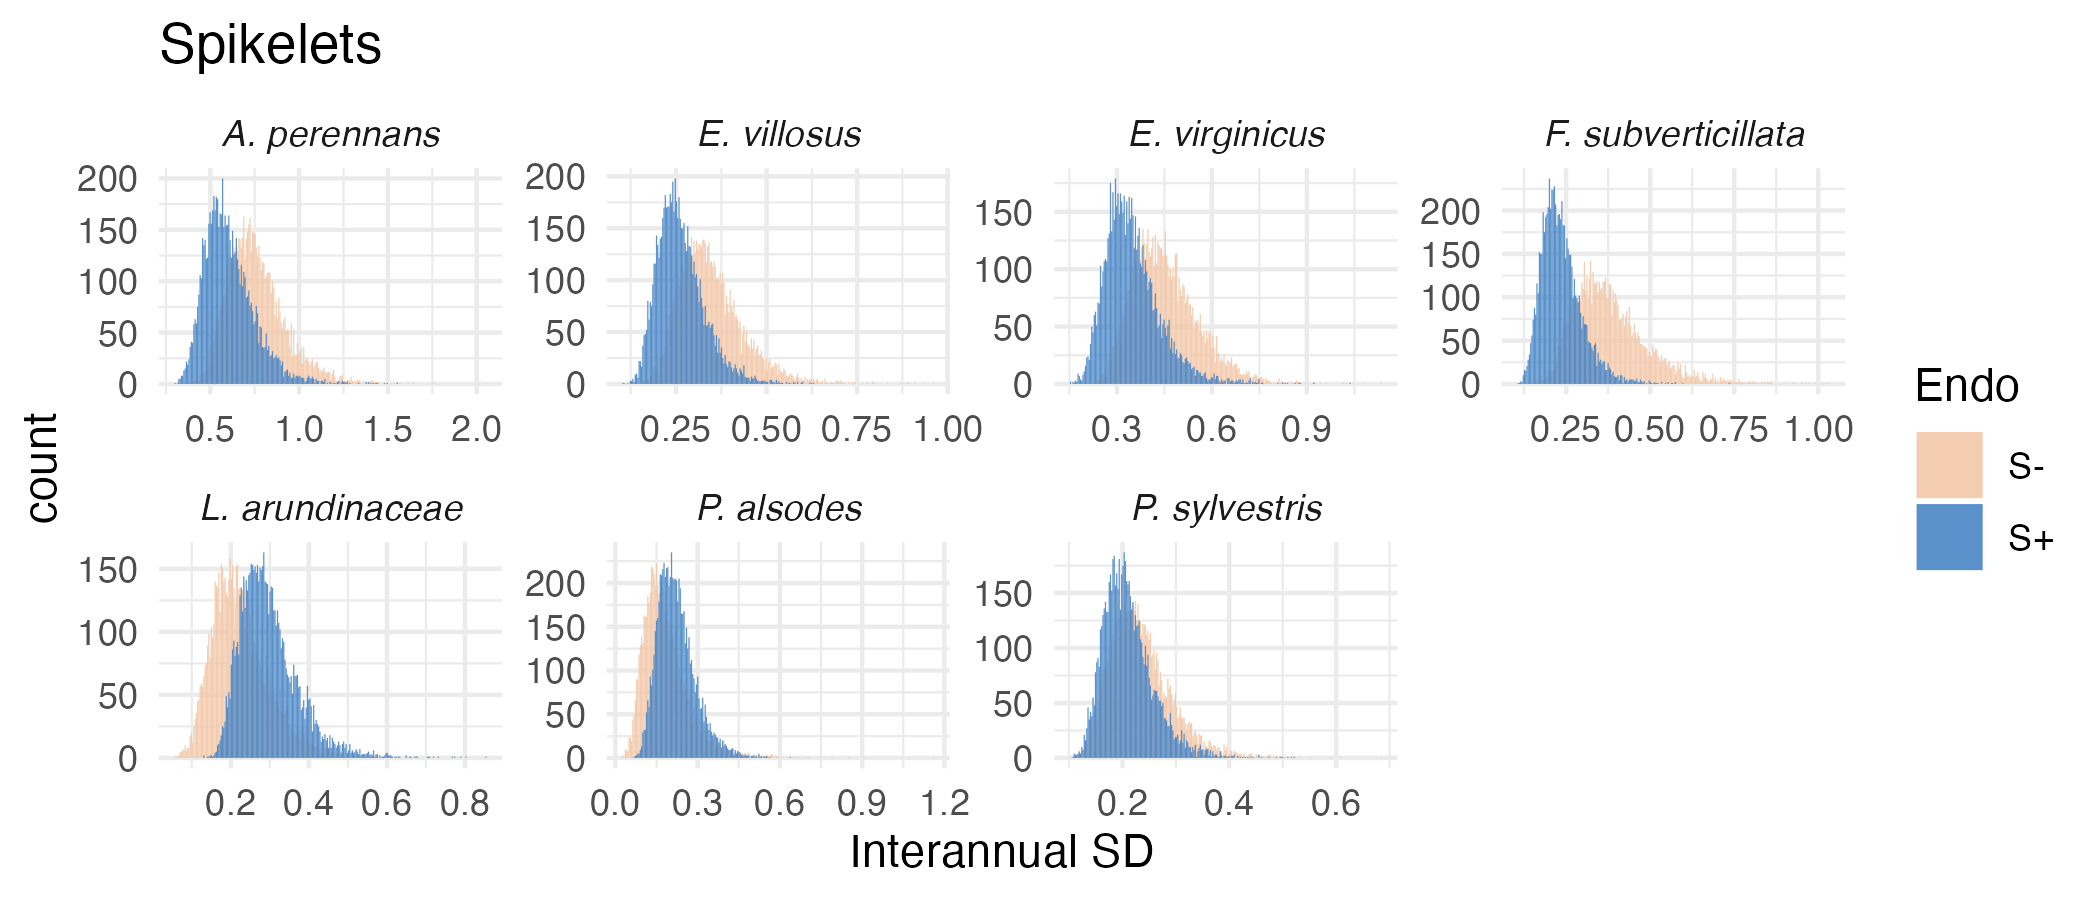
\includegraphics[width=.9\linewidth]{spike_sigmayear_hist.png}
\end{figure}
\noindent {\bf Fig. S17.} \textbf{Posterior distributions of the standard deviations of interannual year effects for spikelets per inflorescence.} Histograms include 7500 post-warmup MCMC samples for symbiotic (S+; blue) and symbiont-free (S-; tan) plants from fitted vital rate model.


\begin{figure}[H]
	\centering
	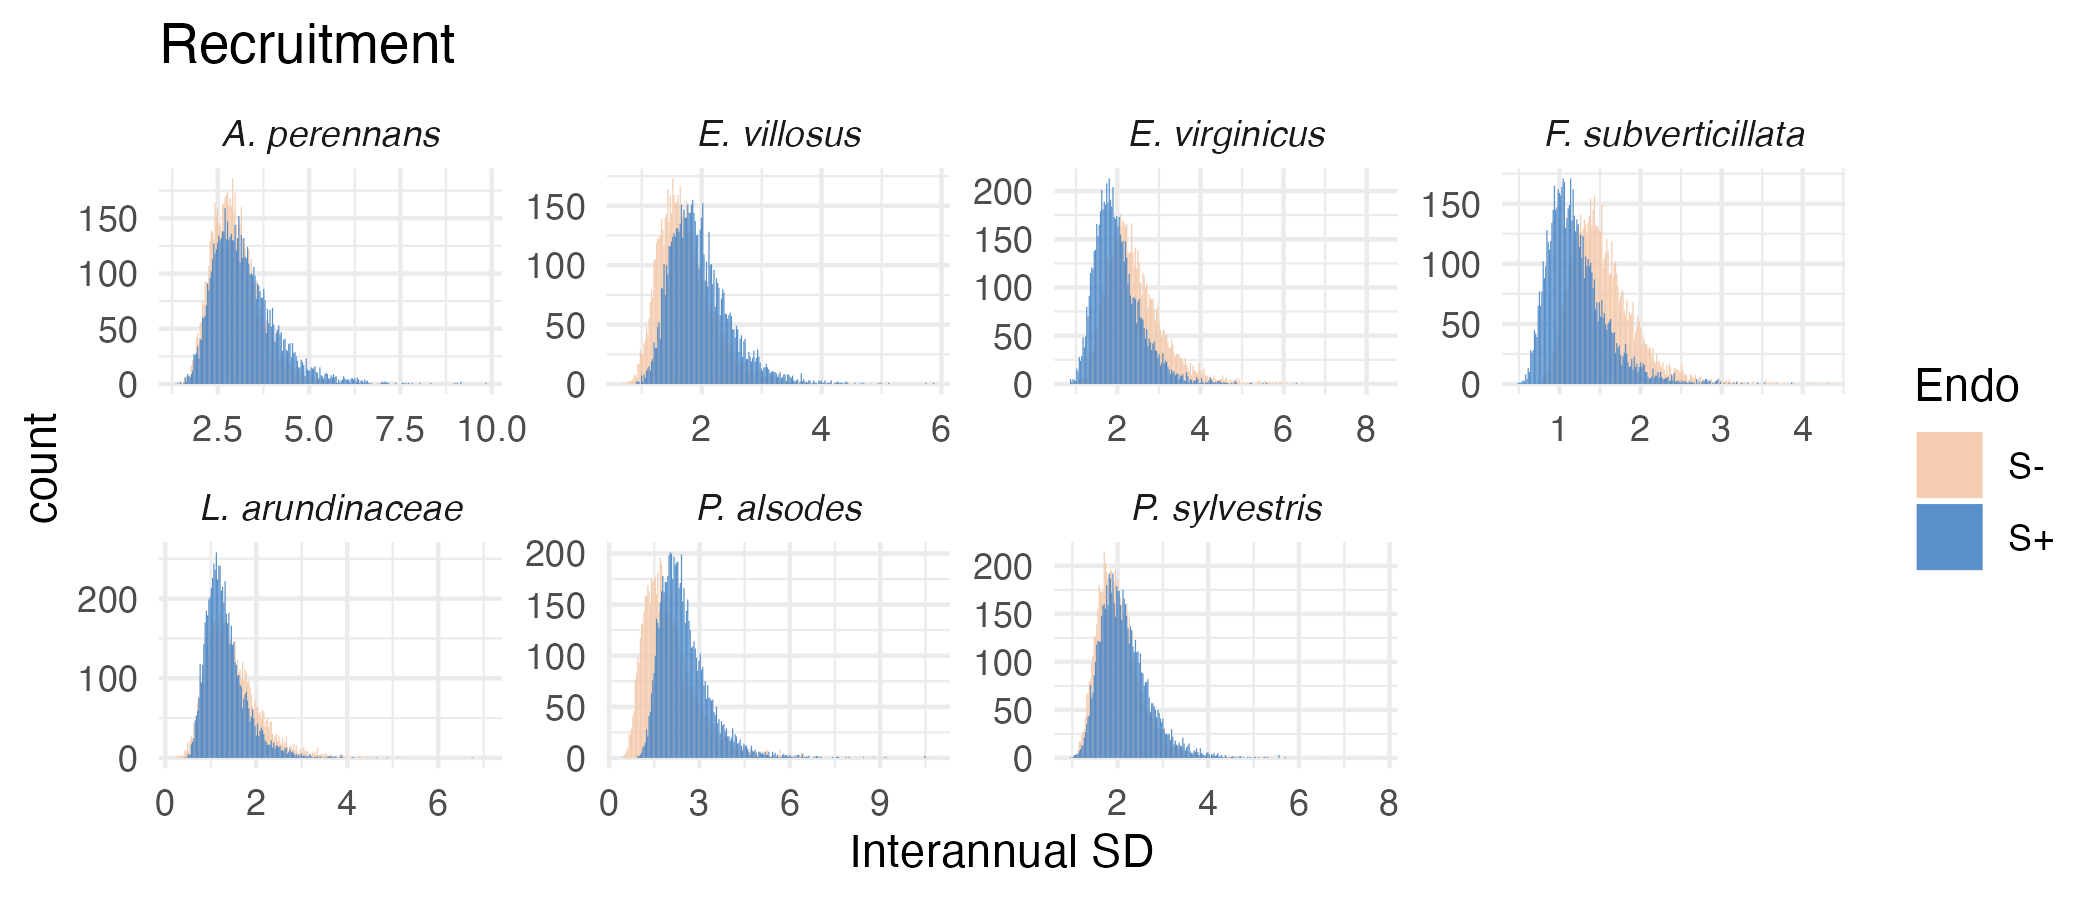
\includegraphics[width=.9\linewidth]{recruit_sigmayear_hist.png}
\end{figure}
\noindent {\bf Fig. S18.} \textbf{Posterior distributions of the standard deviations of interannual year effects for recruitment.} Histograms include 7500 post-warmup MCMC samples for symbiotic (S+; blue) and symbiont-free (S-; tan) plants from fitted vital rate model.

\newpage



\begin{figure}
	\centering
	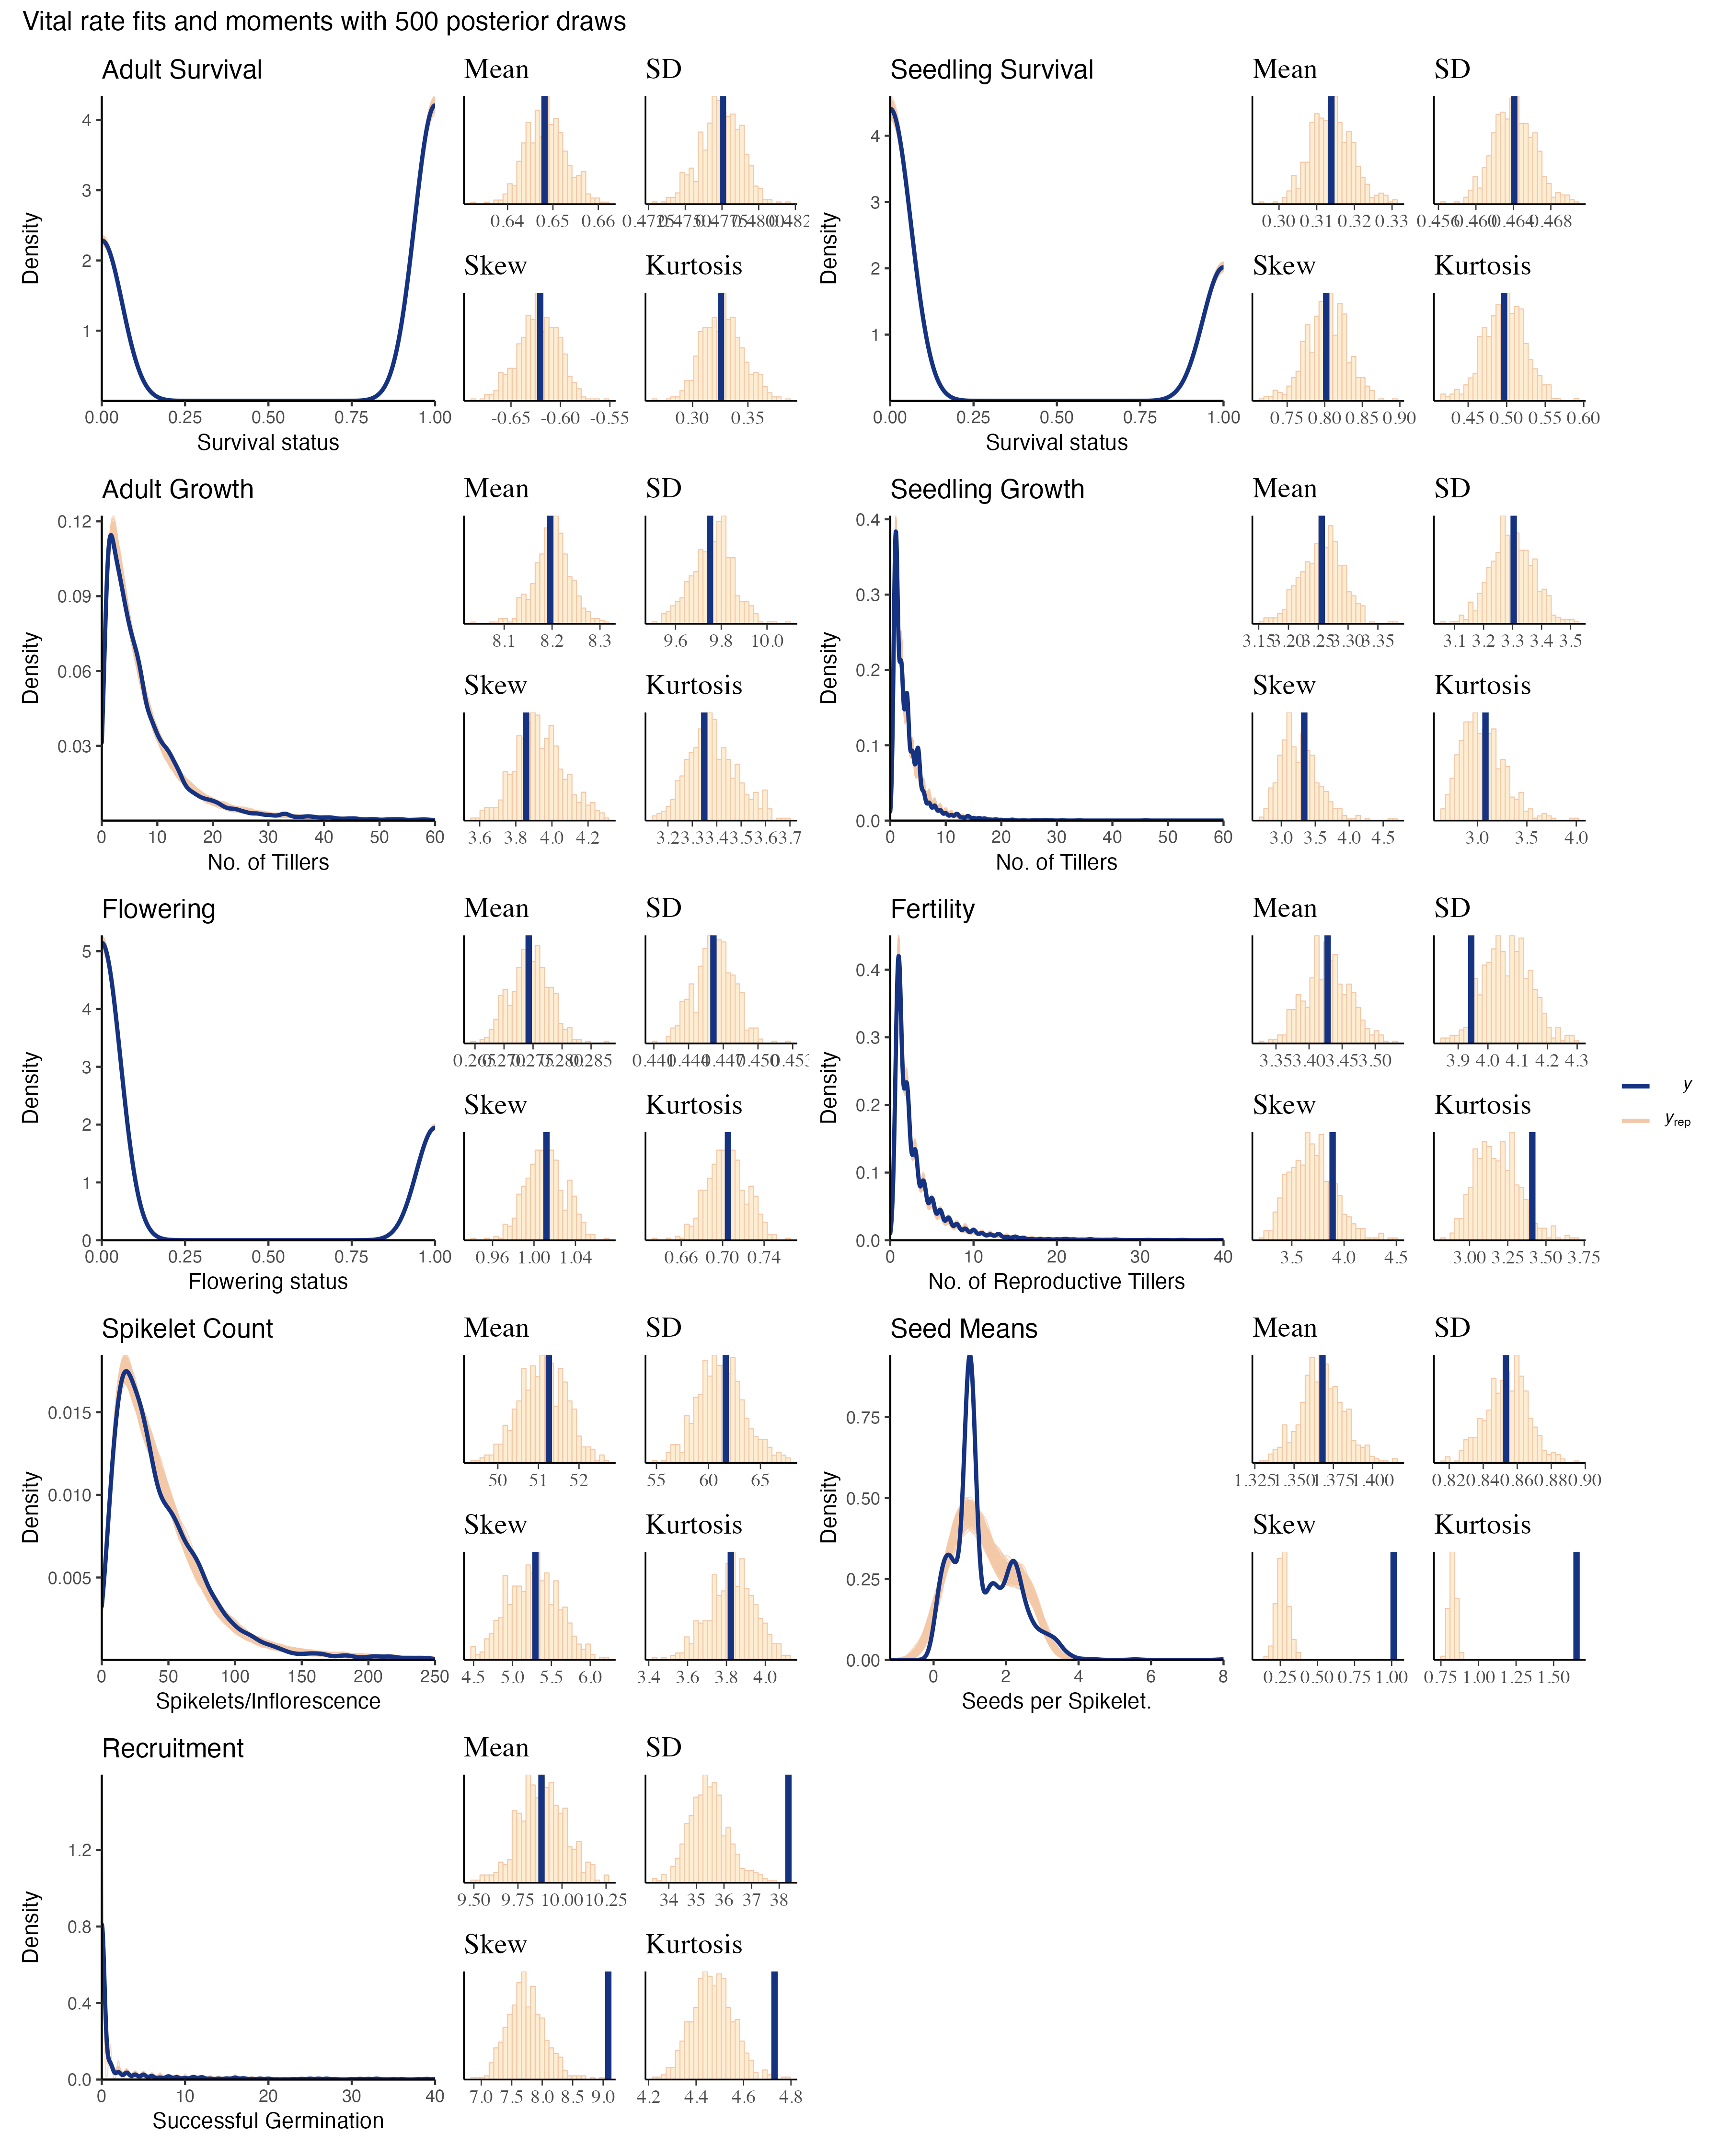
\includegraphics[width=.7\linewidth]{fitsandmoments_plot.png}
\end{figure}
\noindent {\bf Fig. S19.} \textbf{Consistency between real data and simulated values indicates that fitted models describe the data well.} Graphs show posterior predictive check for statistical models of demographic vital rates. Lines show density distributions of observed data (blue line) compared to data simulated from fitted models (tan lines) generated from 500 draws from posterior distributions of model parameters. 
\newpage

\begin{figure}
	\centering
	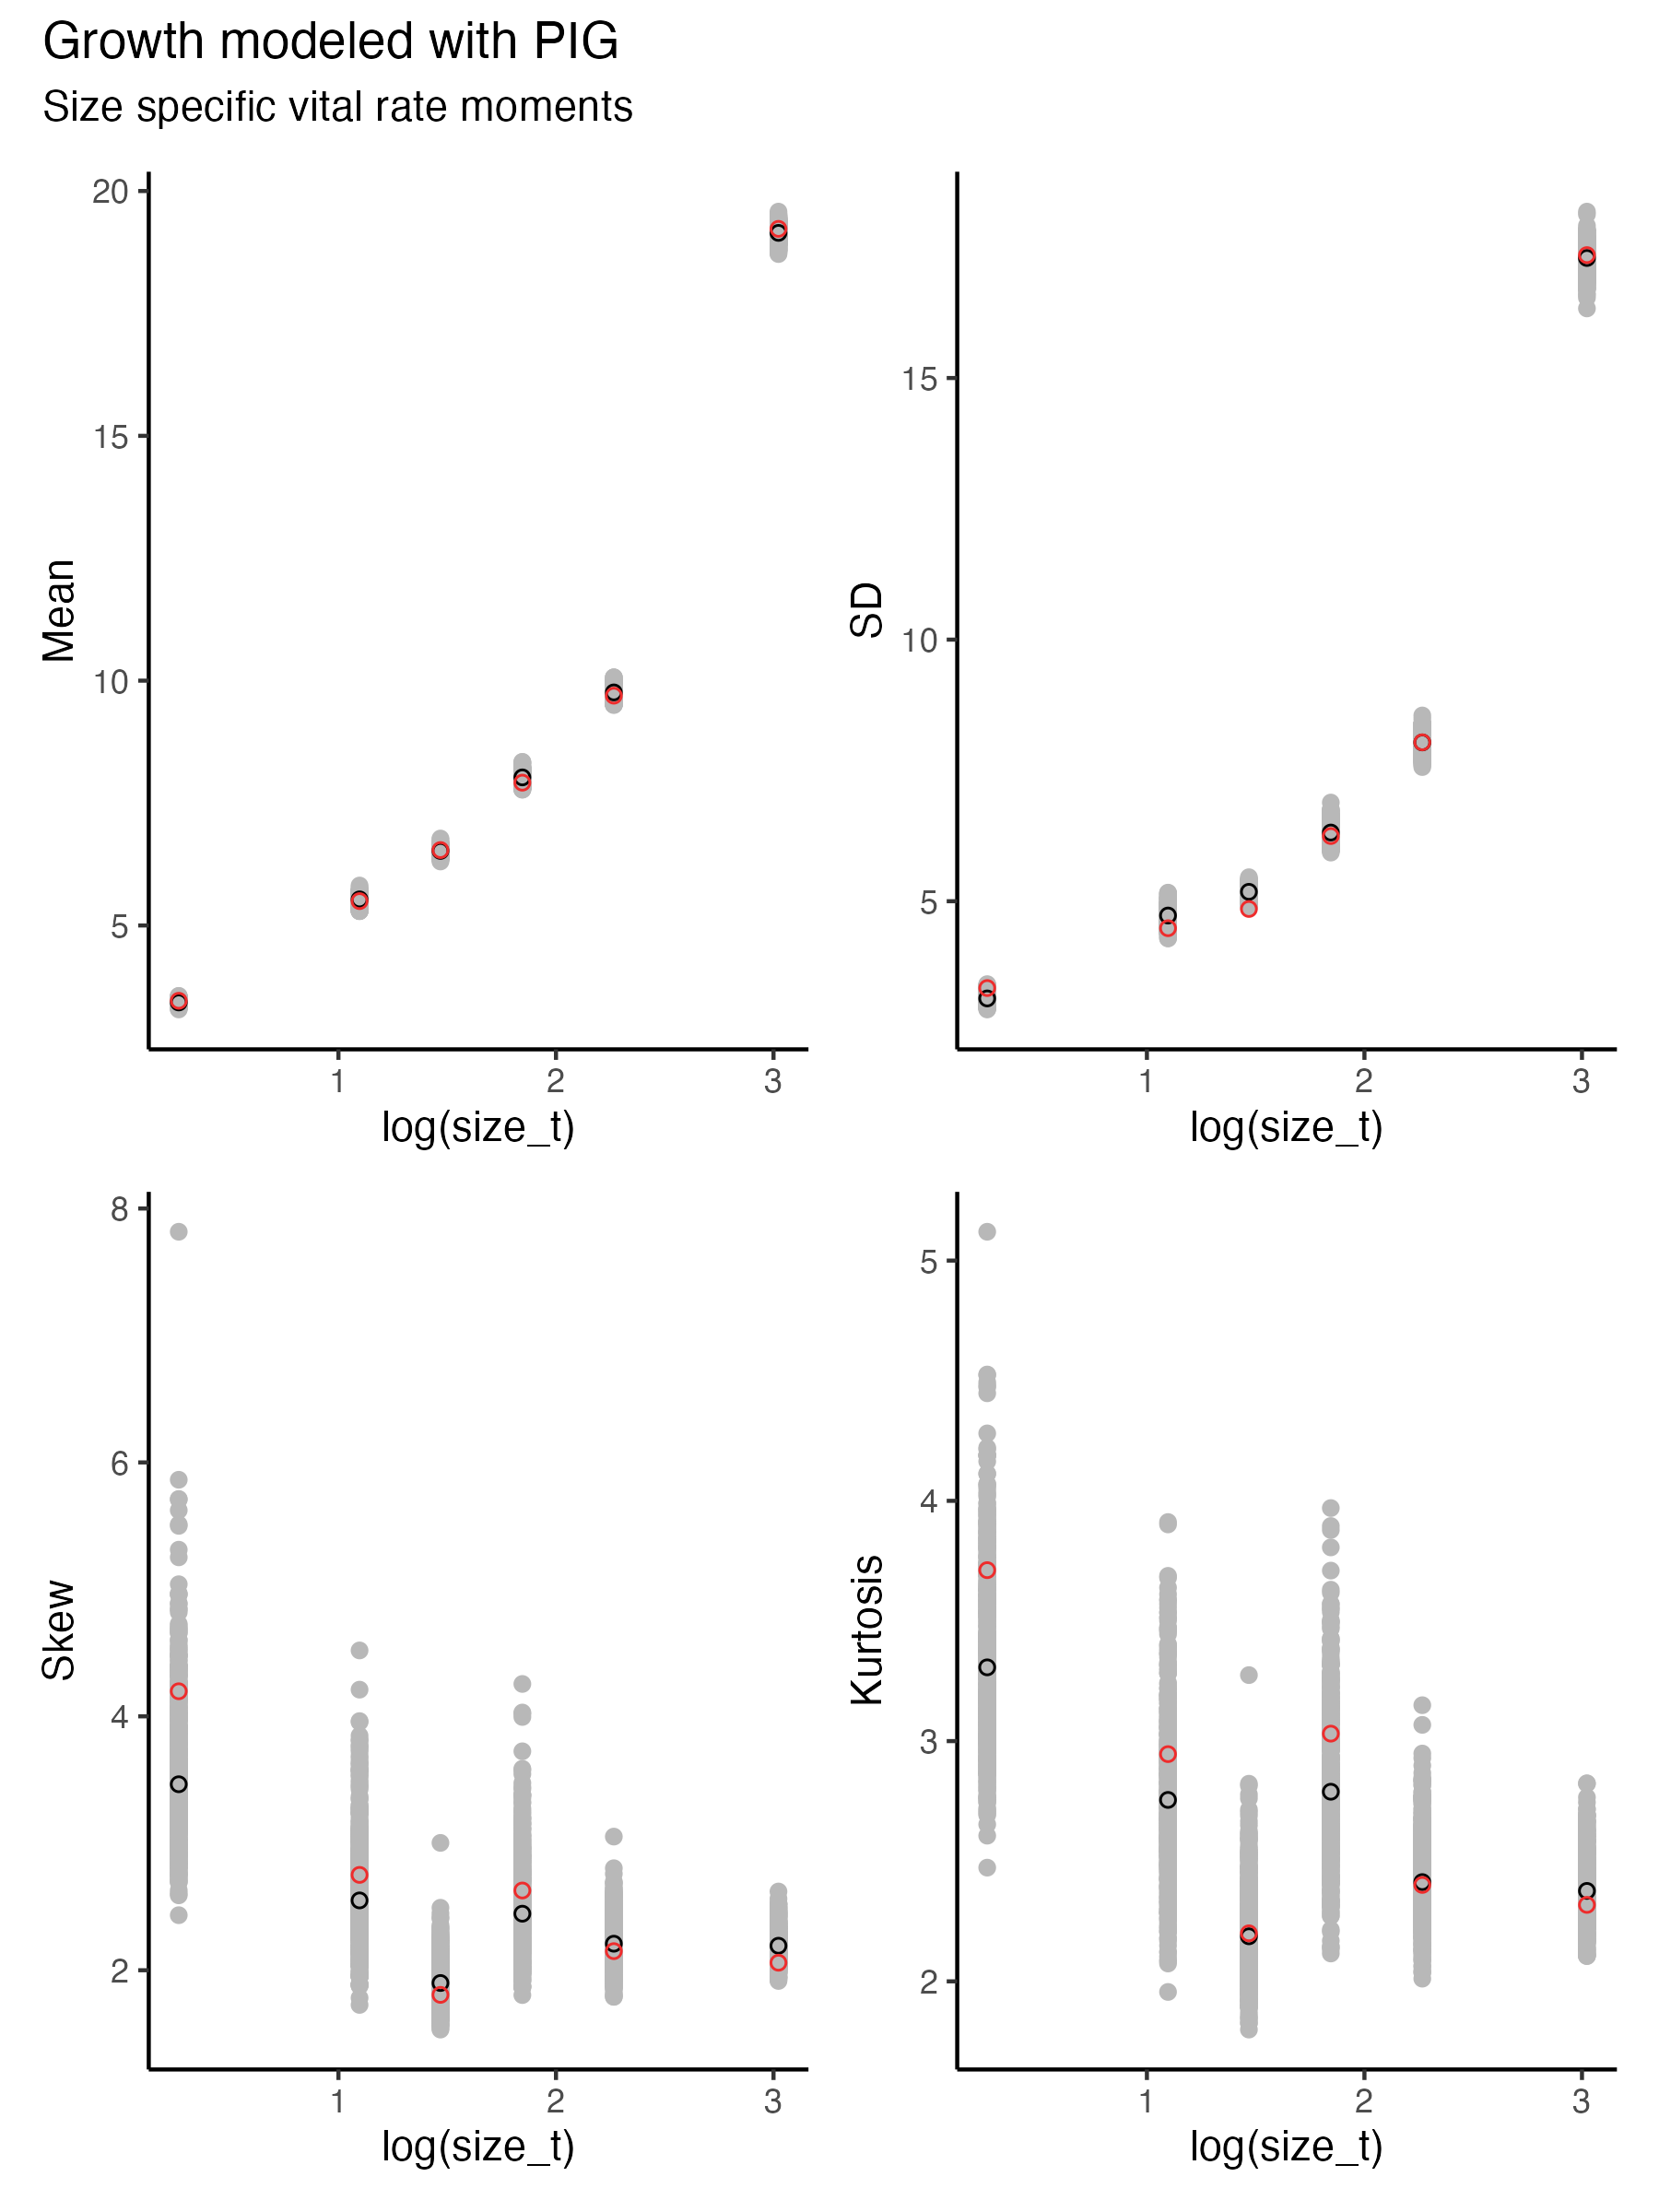
\includegraphics[width=.6\linewidth]{size_ppc_plot.png}
\end{figure}
\noindent {\bf Fig. S20.} \textbf{Consistency between real data and fitted values across sizes indicates that the growth model is accurately capturing size dependence} Graphs of posterior predictive check for mean and higher moments of the growth model across size. Points show the value of statistical moments binned across size for the observed data (red circles) compared to the simulated datasets (grey circles) and the median of the simulated values (black circles) generated from 500 posterior draws from the fitted model. 
\newpage

\begin{figure}
	\centering
	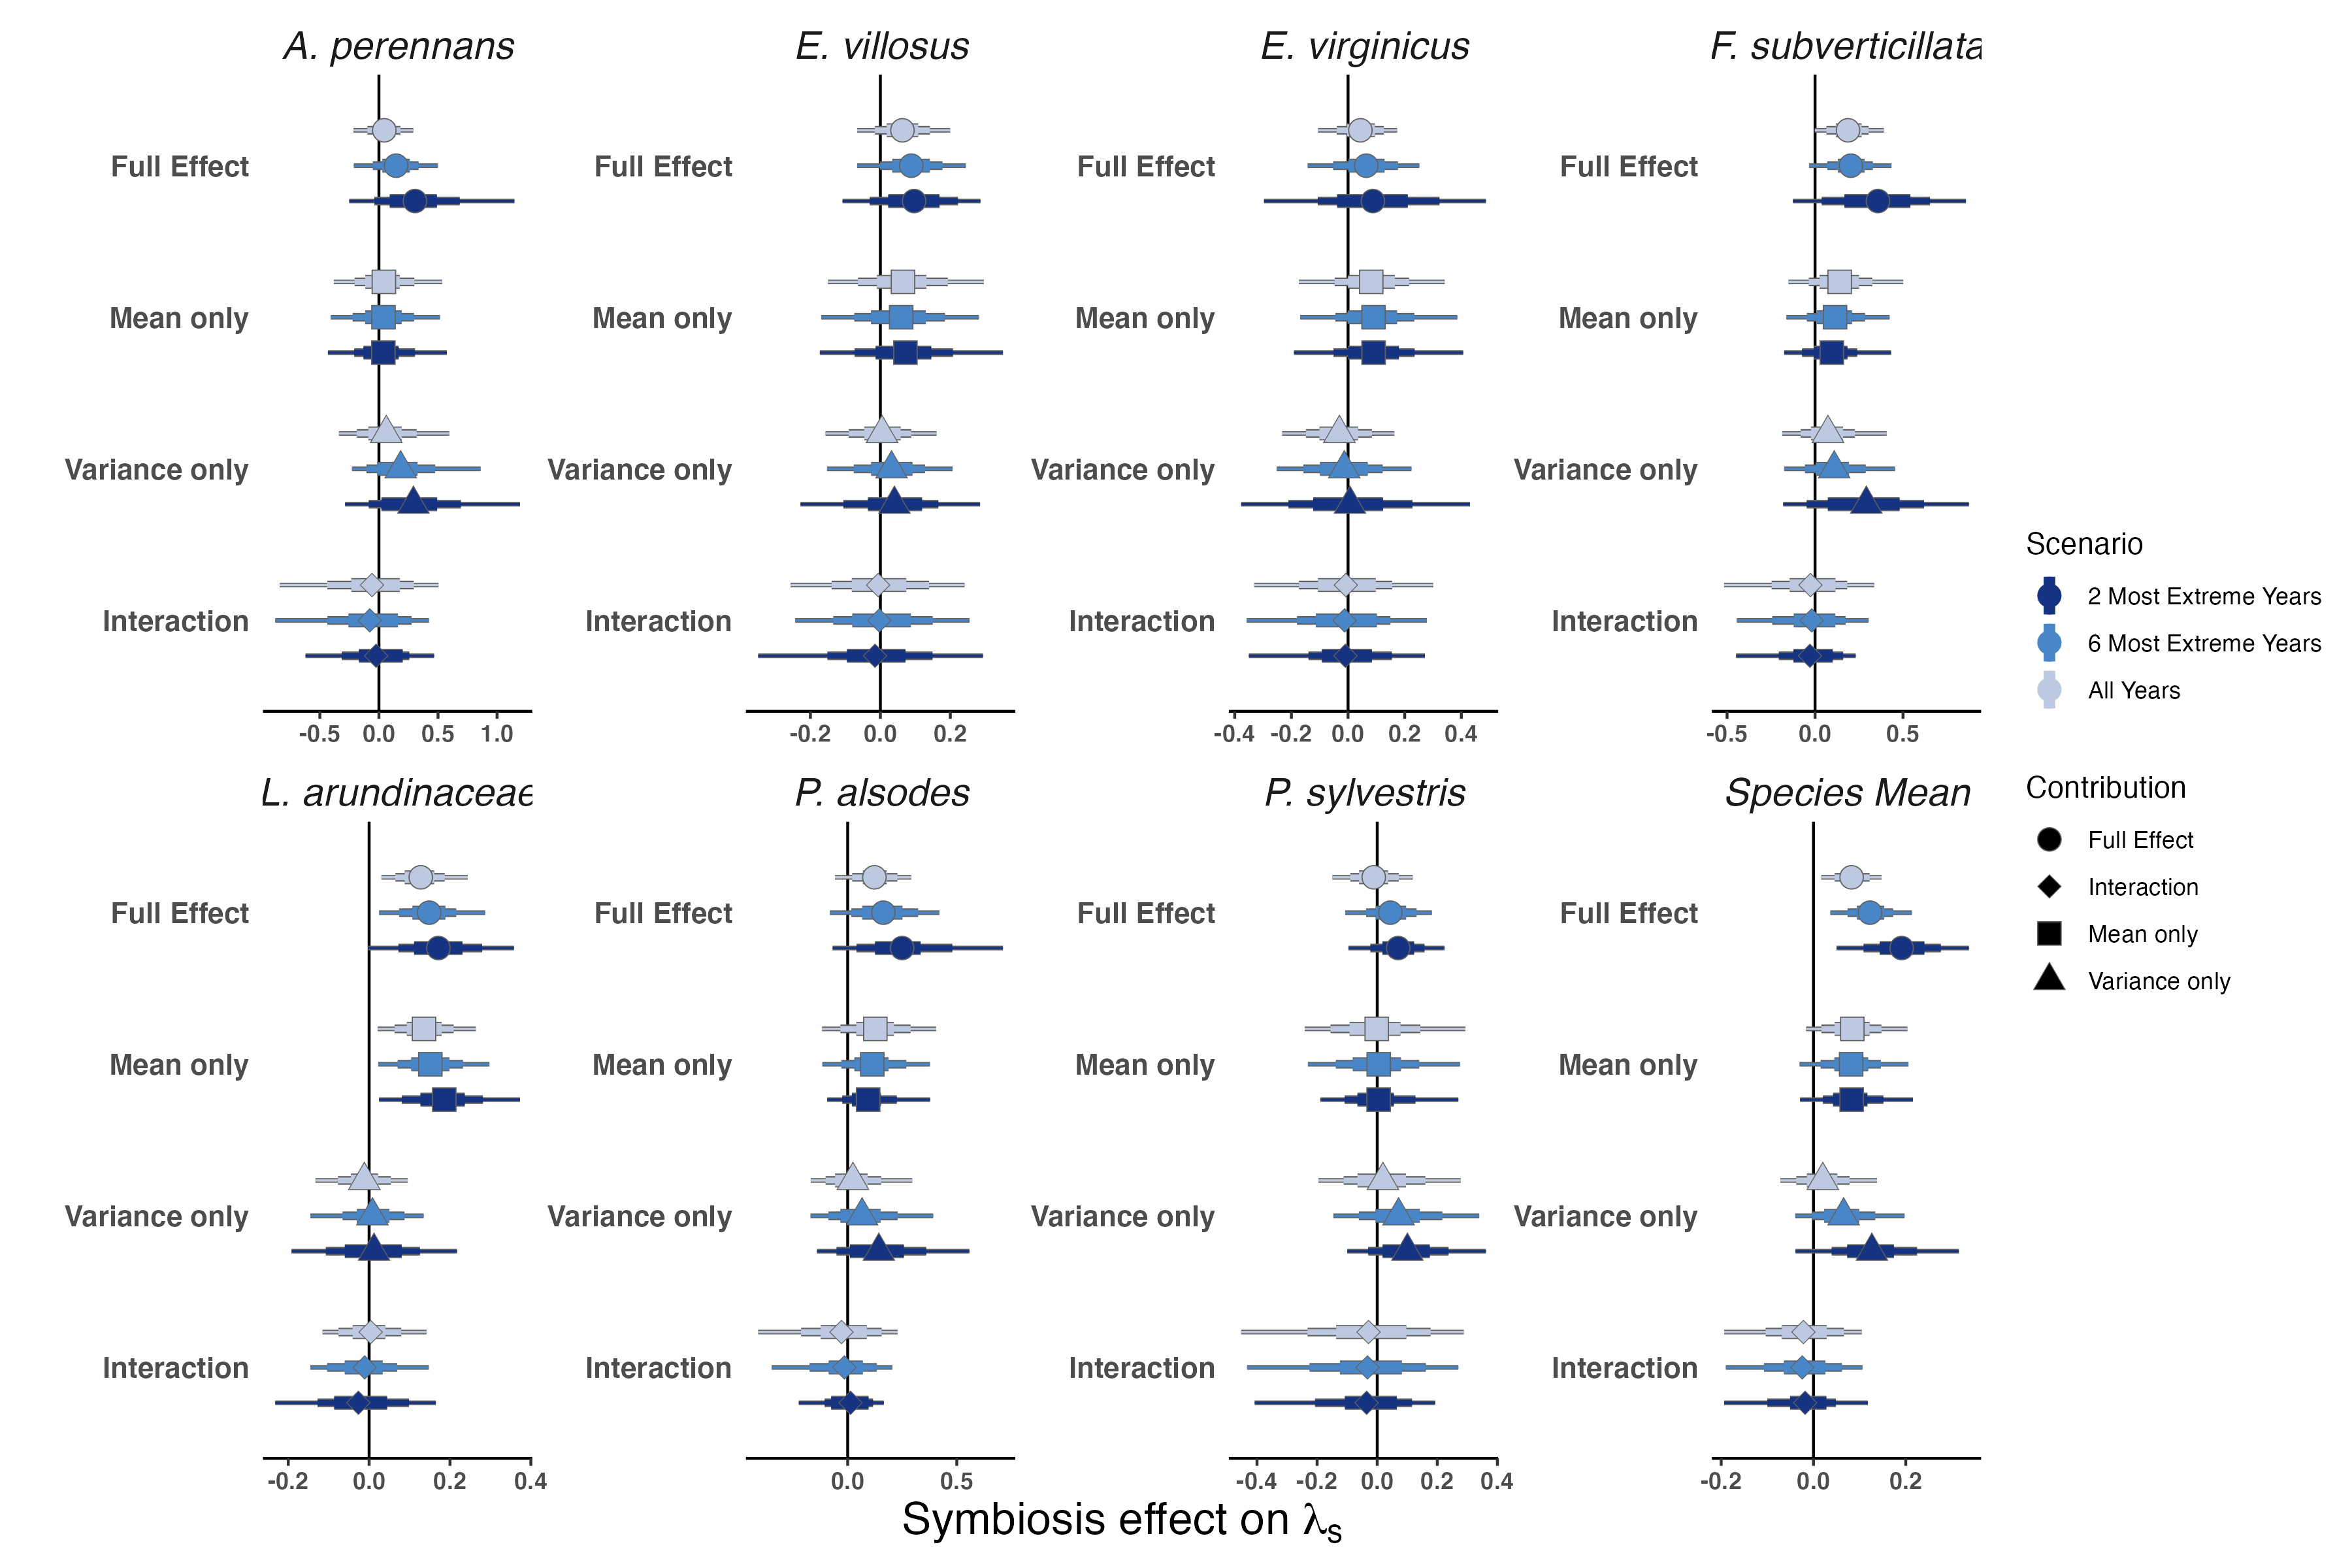
\includegraphics[width=\linewidth]{contributions_obs_plot.png}
\end{figure}
\noindent {\bf Fig. S21.} \textbf{Endophyte contributions to stochastic growth rates under observed and elevated variance across species.} The total effect of endophytes (circle) comes from mean benefits (square) and variance buffering (triangle) as well as the interaction between mean and variance effects (diamond). Shapes indicate the posterior mean of each contribution, along with bars for the 50, 75 and 95 \% credible intervals.  Under scenarios of increasing variance, represented by increasing color intensity, effects of variance buffering increase leading to a more mutualistic symbiosis.
\newpage

\begin{figure}
	\centering
	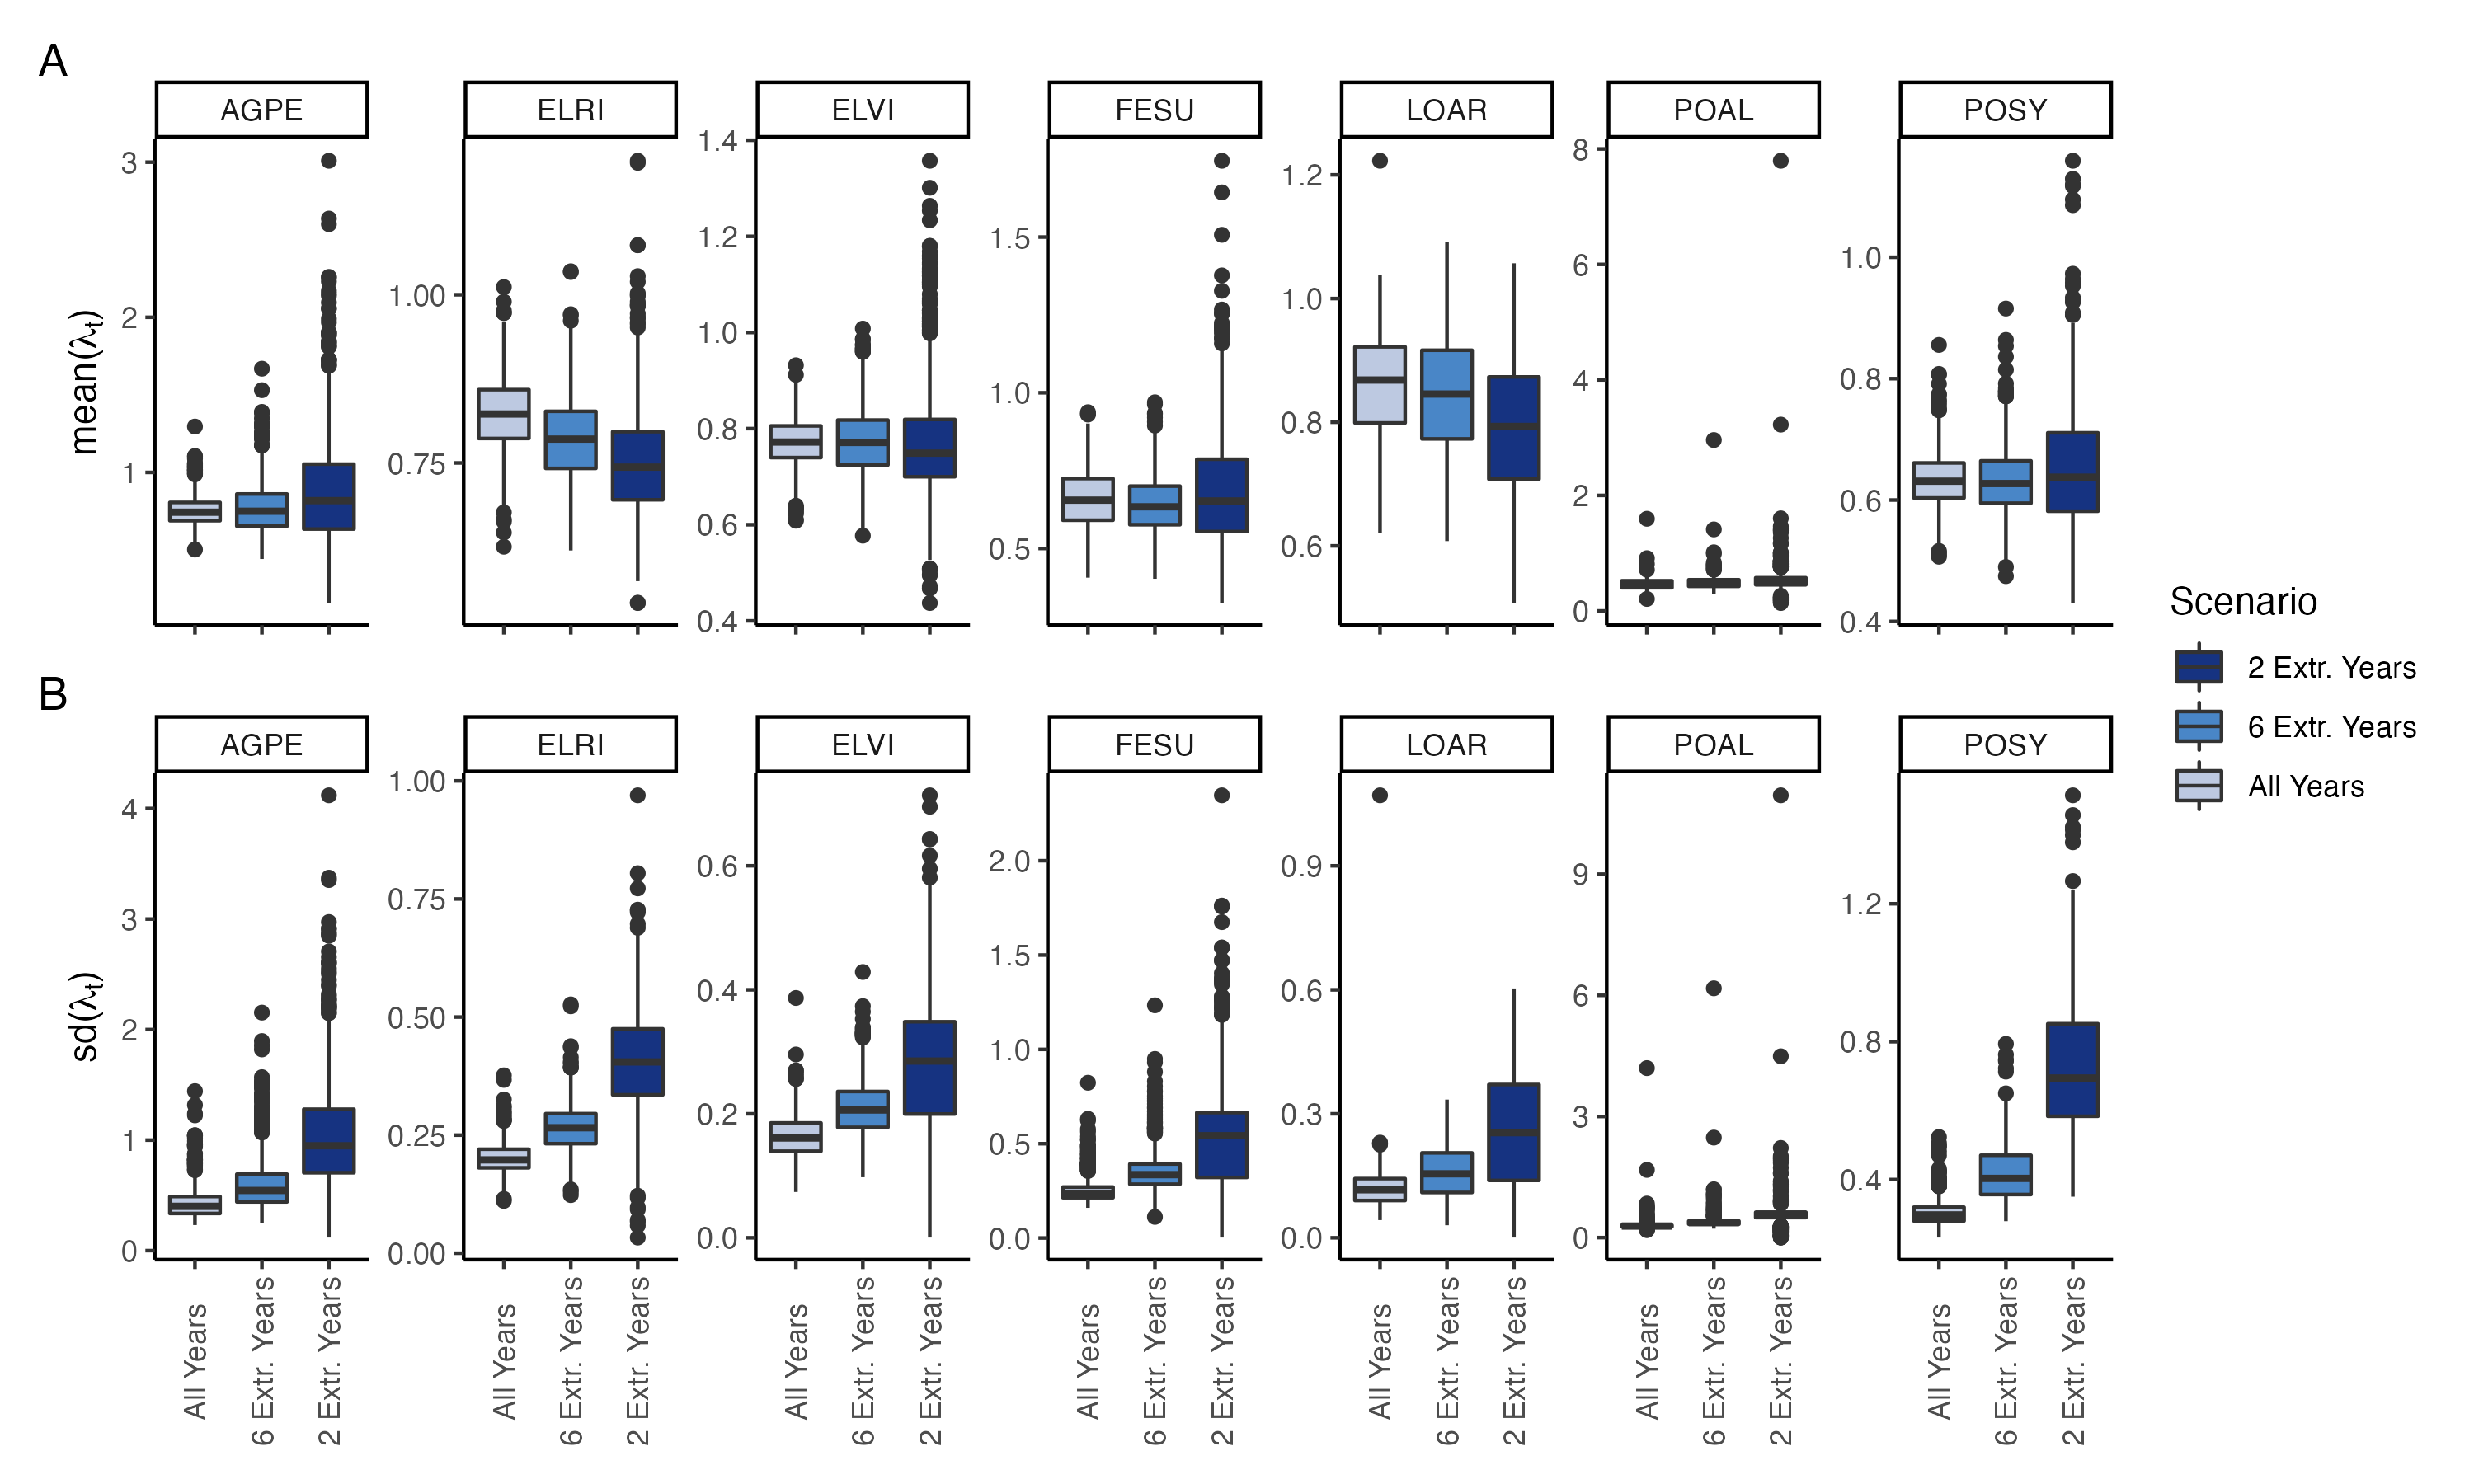
\includegraphics[width=\linewidth]{sim_boxplots.png}
\end{figure}
\noindent {\bf Fig. S22.} \textbf{(A) Mean and (B) standard deviation of annual growth rate values during simulation scenarios.} Each scenario selects from observed transition matrixes, increasing the variance by selecting either all observed years, or a set (6 or 2 years) that have the highest and lowest growth rates for symbiont-free populations.
\newpage


\begin{figure}
	\centering
	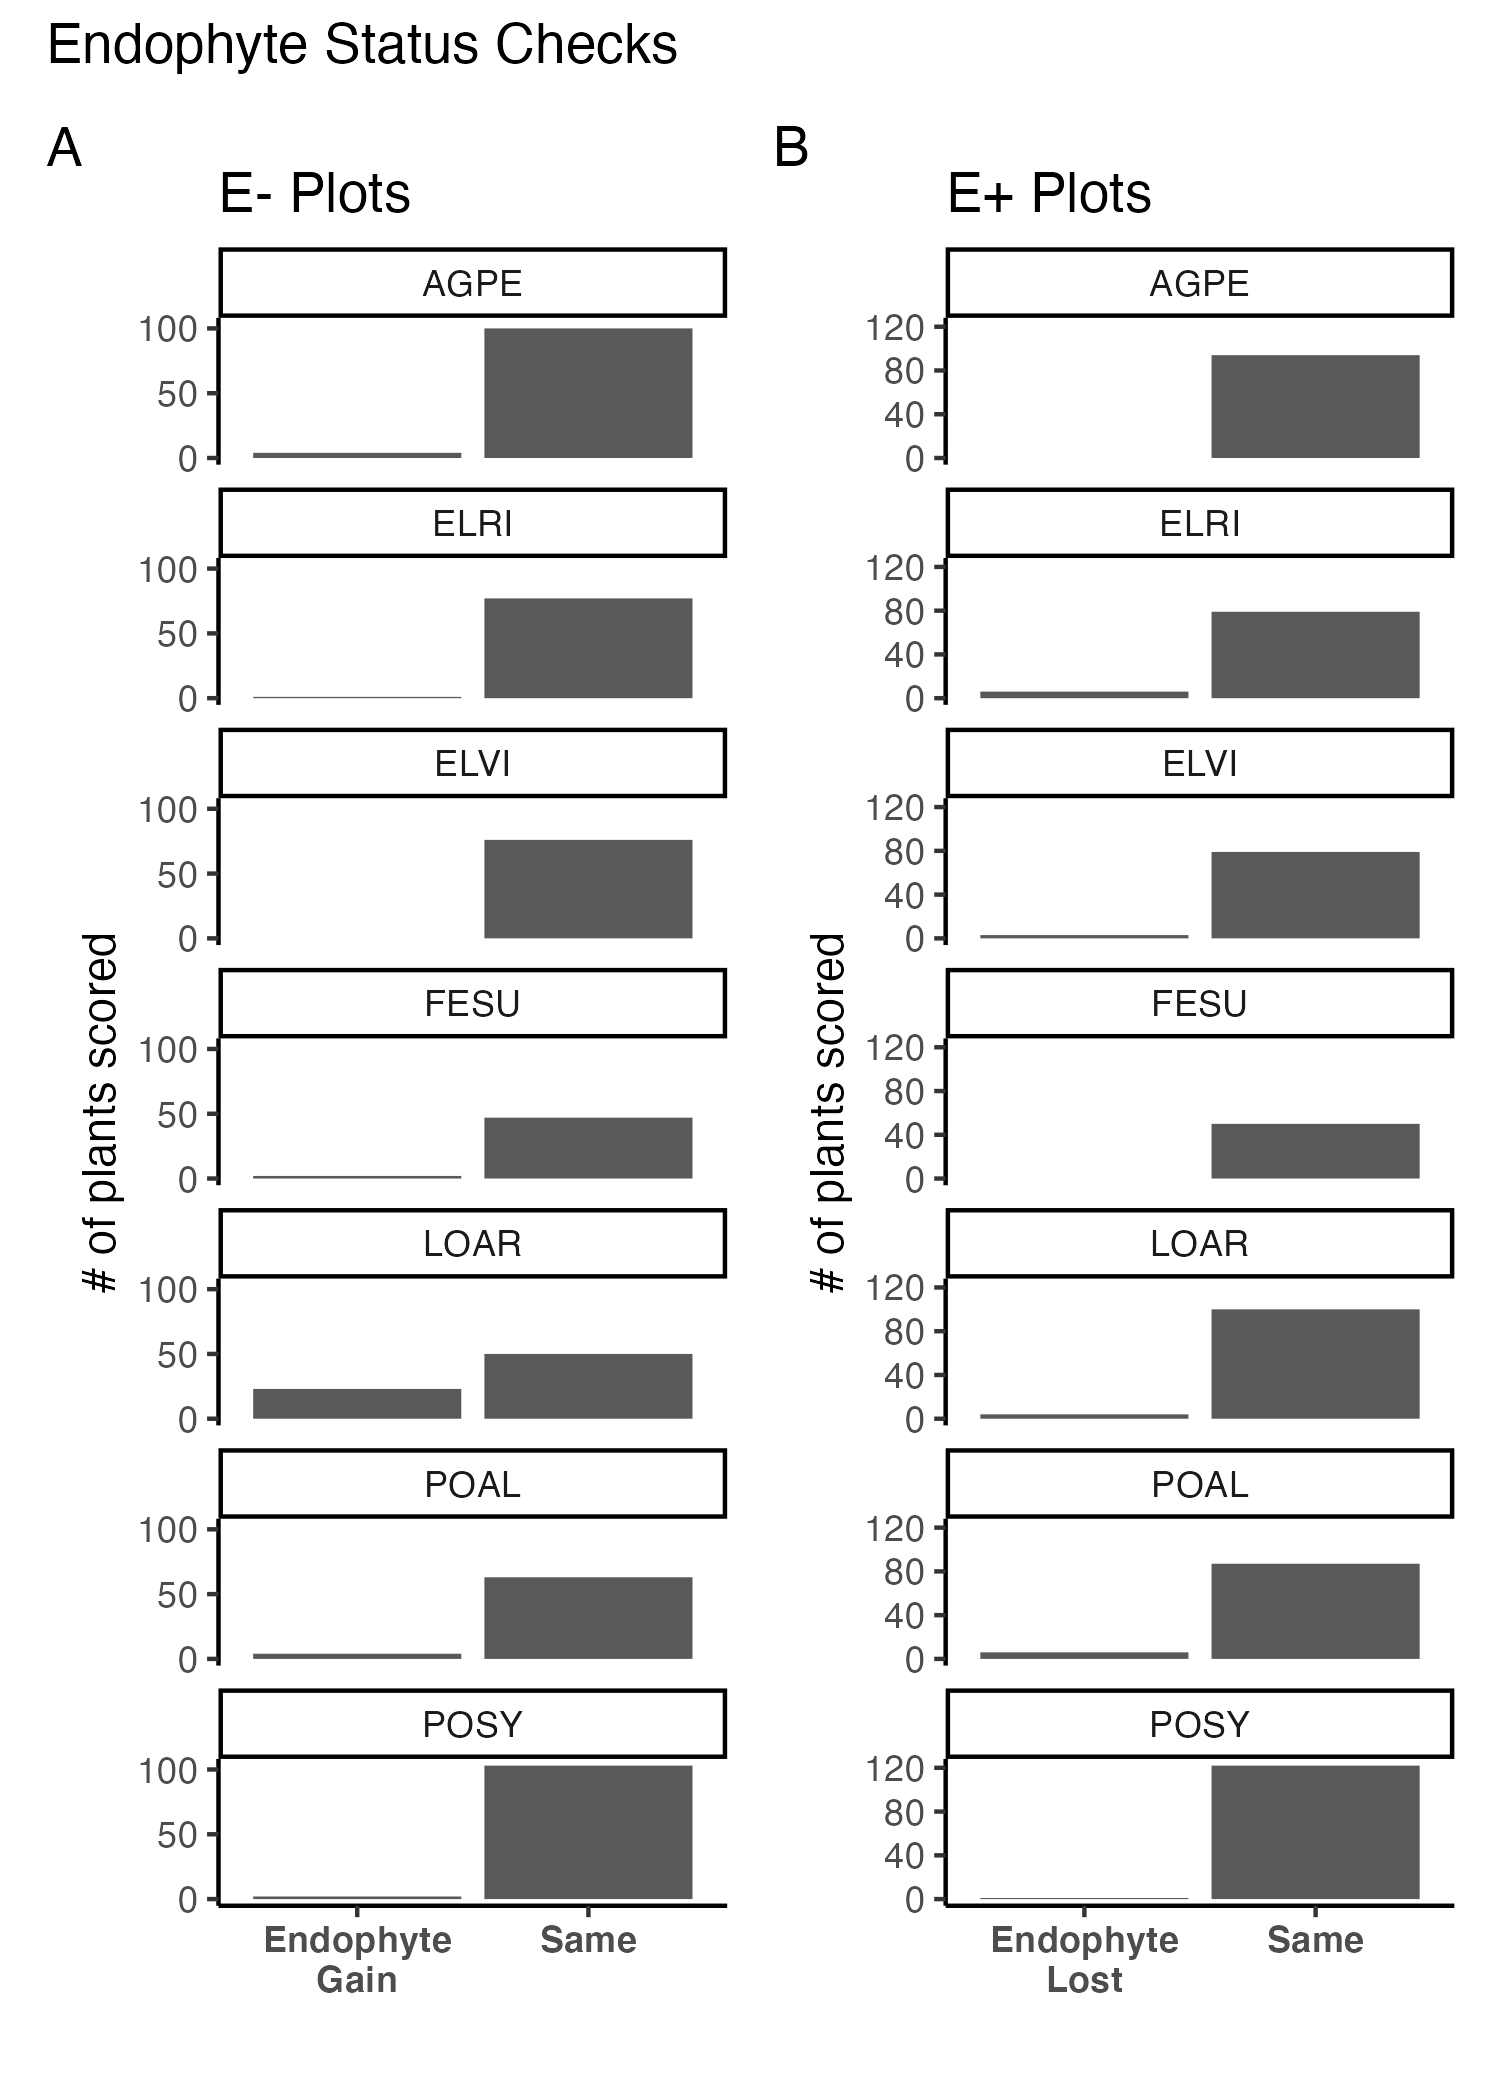
\includegraphics[width=.6\linewidth]{endo_check_plot.png}
\end{figure}
\noindent {\bf Fig. S23.} \textbf{Faithfulness of experimental plots to assigned endophyte status.} Counts of plants scored with leaf peels or seed squashes to check the faithfulness of recruits to the assigned plot-level endophyte status. (A) Endophytic plants may be gained in initially S- plots, or (B) lost in initially S+ plots.
\newpage

\begin{figure}
	\centering
	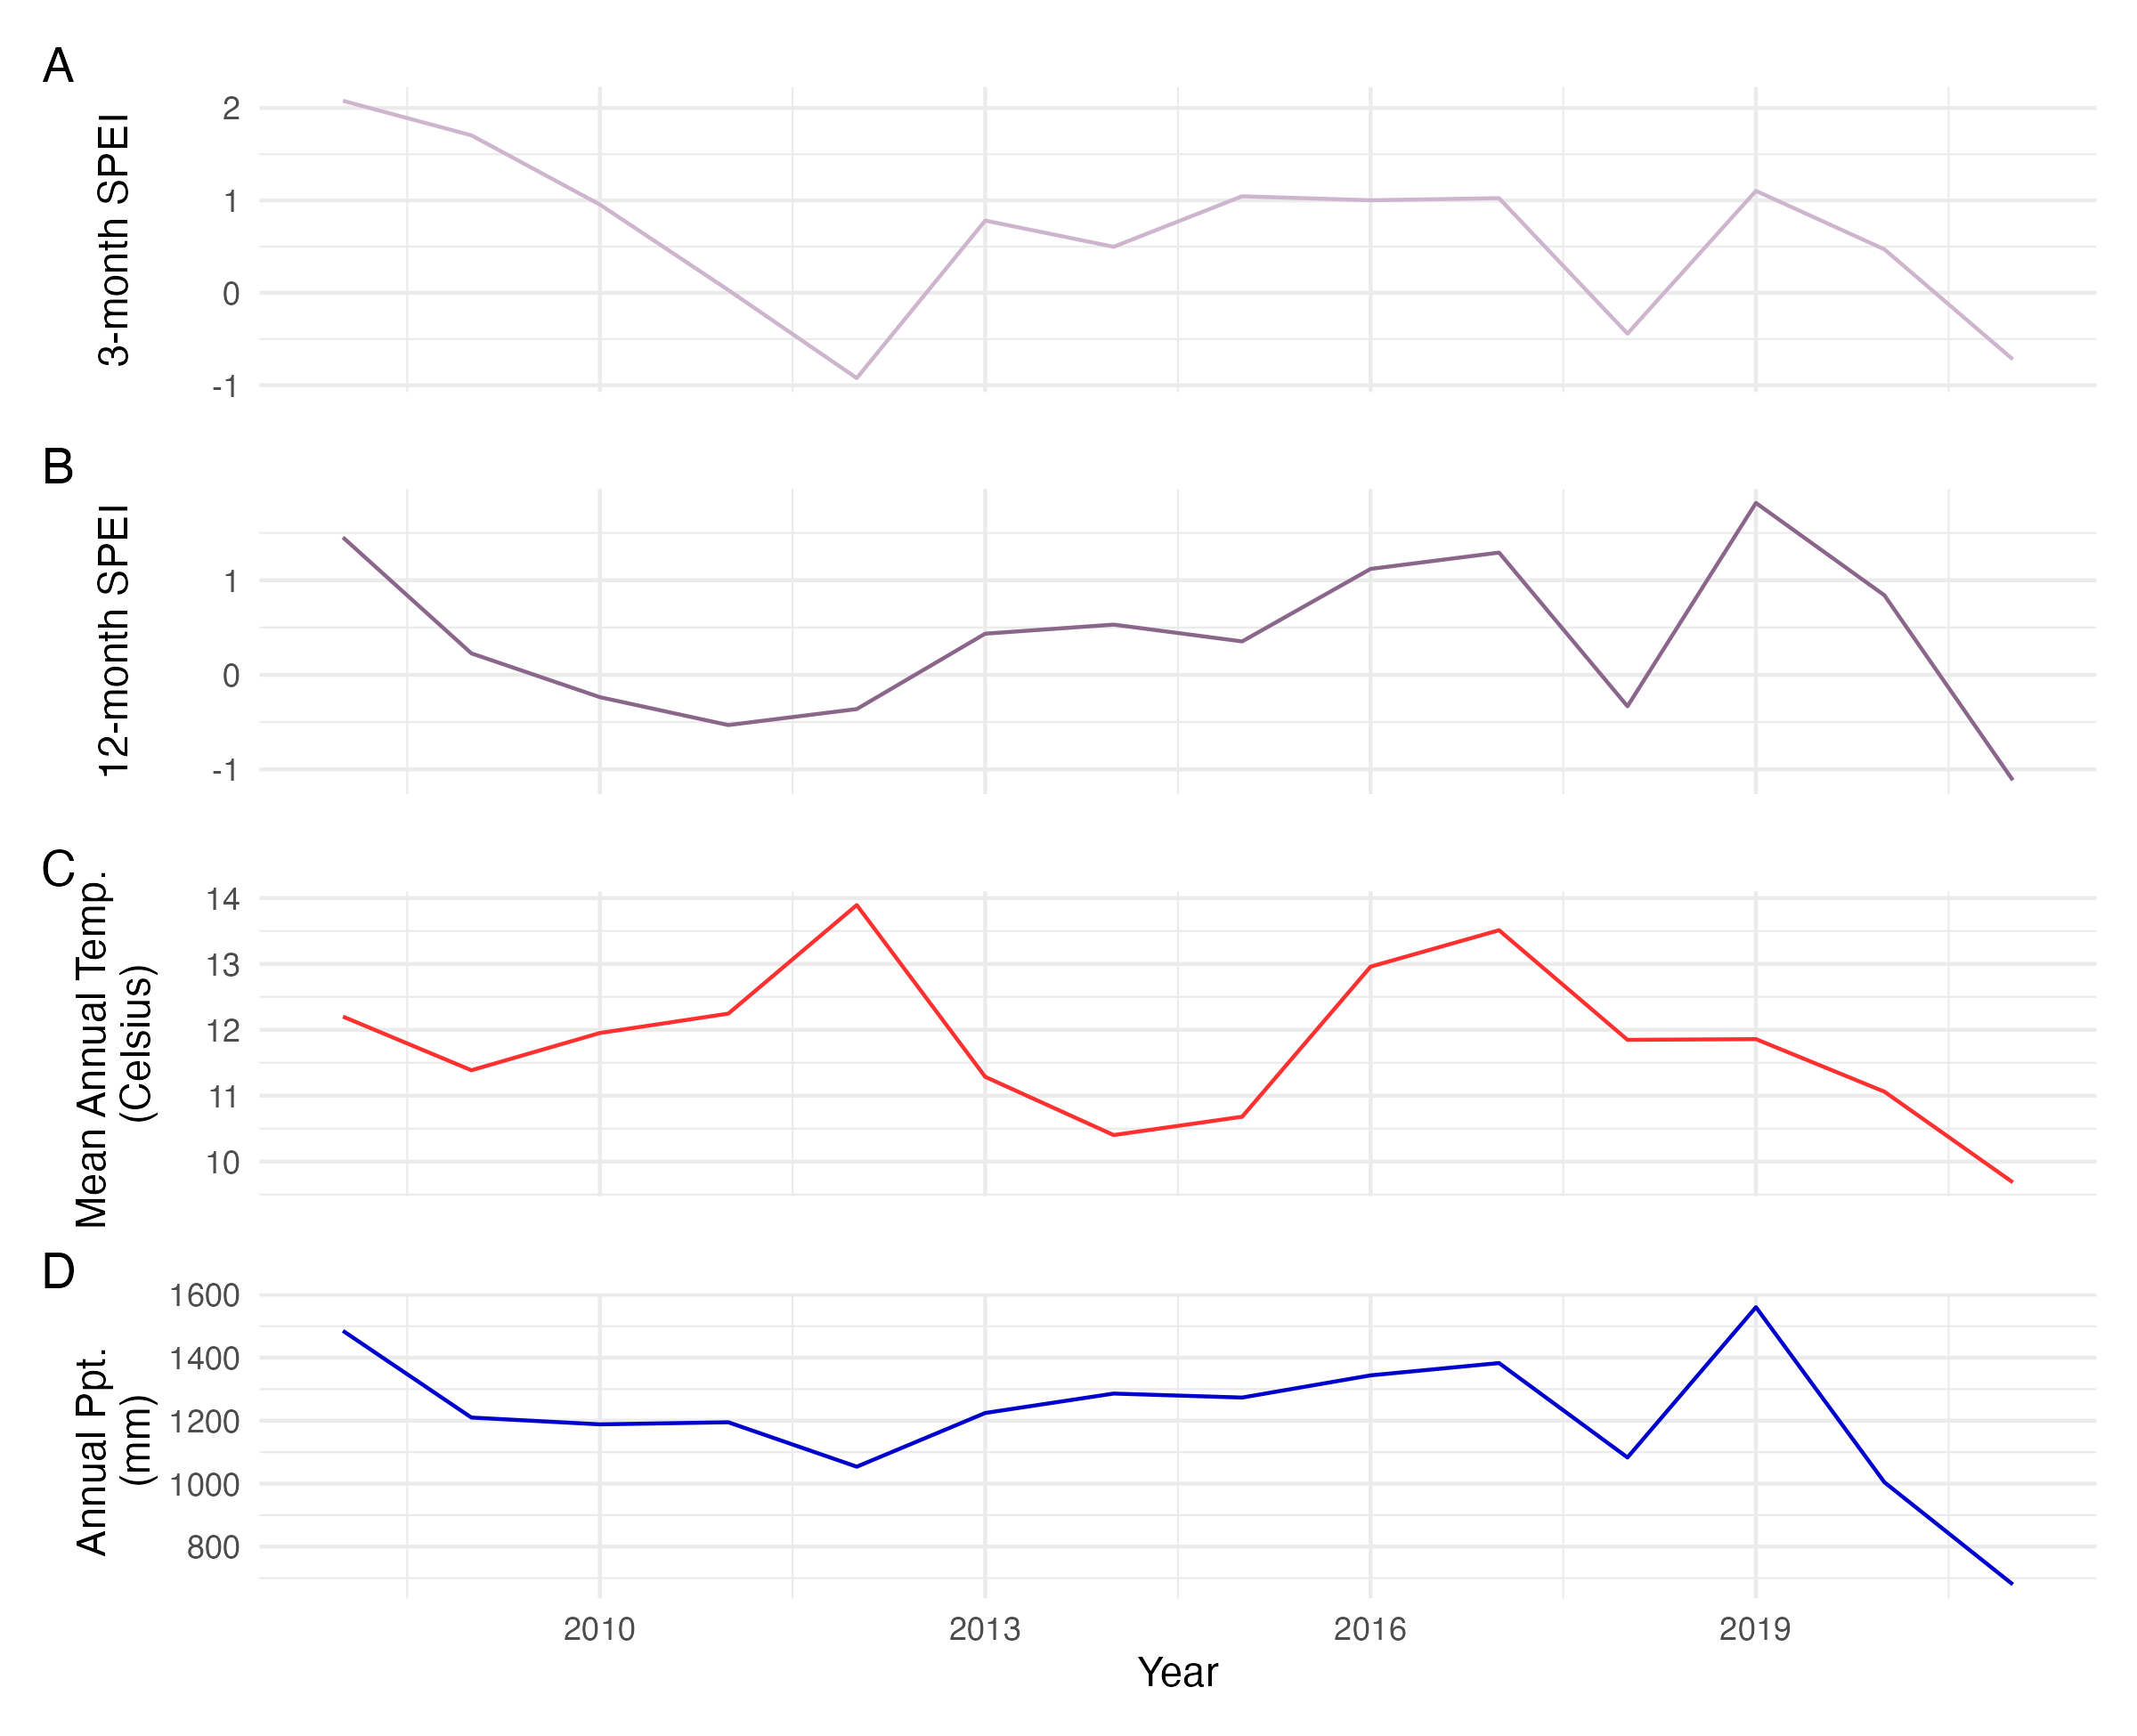
\includegraphics[width=\linewidth]{climate_plot.png}
\end{figure}
\noindent {\bf Fig. S24.} \textbf{Weather station time-series for Bloomington, IN.} The Seasonal Precipitation-Evapotranspiration Index (SPEI) calculated for the (A) three month growing season and (B) annually from daily weather station observations of (C) average temperatures and (D) cumulative precipitation. Climatic data shown are determined by the census year centered on the month of July. % when \emph{E. villosus} and \emph{E. virginicus}.
\newpage

\begin{figure}
	\centering
	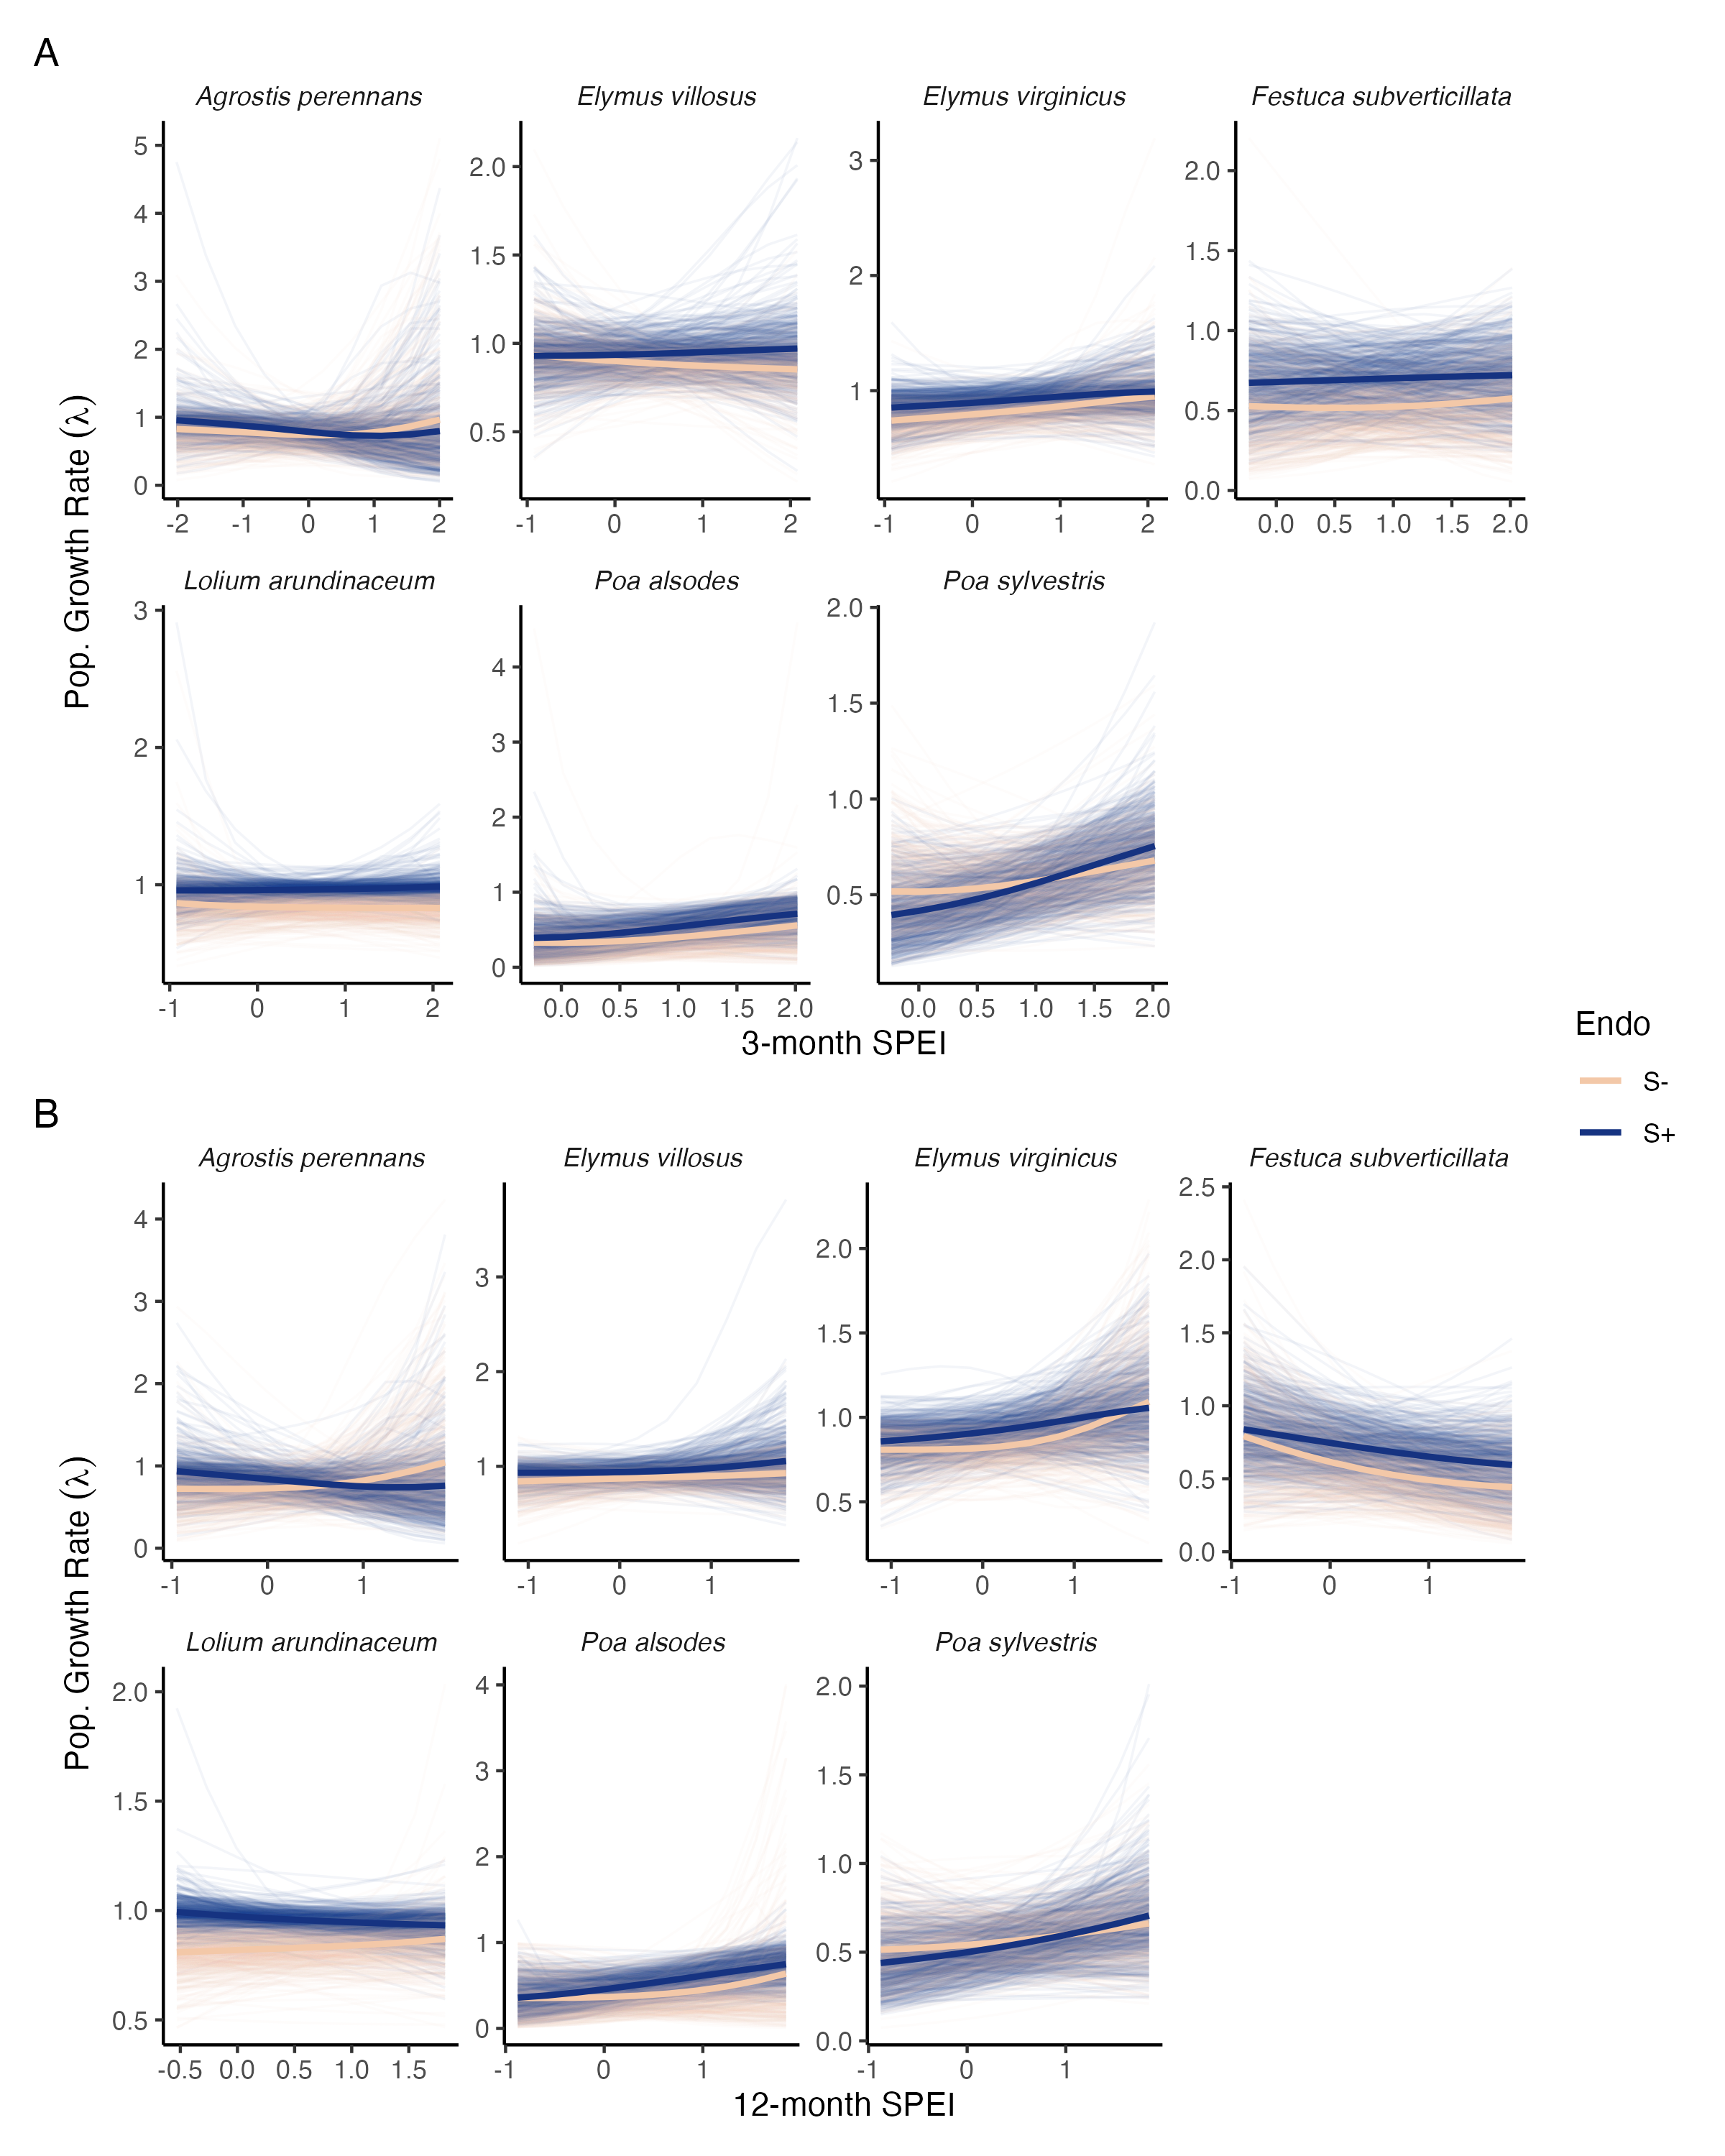
\includegraphics[width=.7\linewidth]{spei_combo_lambda_plot.png}
\end{figure}
\noindent {\bf Fig. S25.} \textbf{Predicted population growth rates across drought indices.} Symbiotic (S+; blue) and symbiont-free (S-; tan) populations respond differently to climate as measured by the (A) 3-month SPEI and (B) 12-month SPEI. Thick lines represent the predicted mean growth rate and thin lines show 500 posterior draws.
\newpage


\begin{figure}
	\centering
	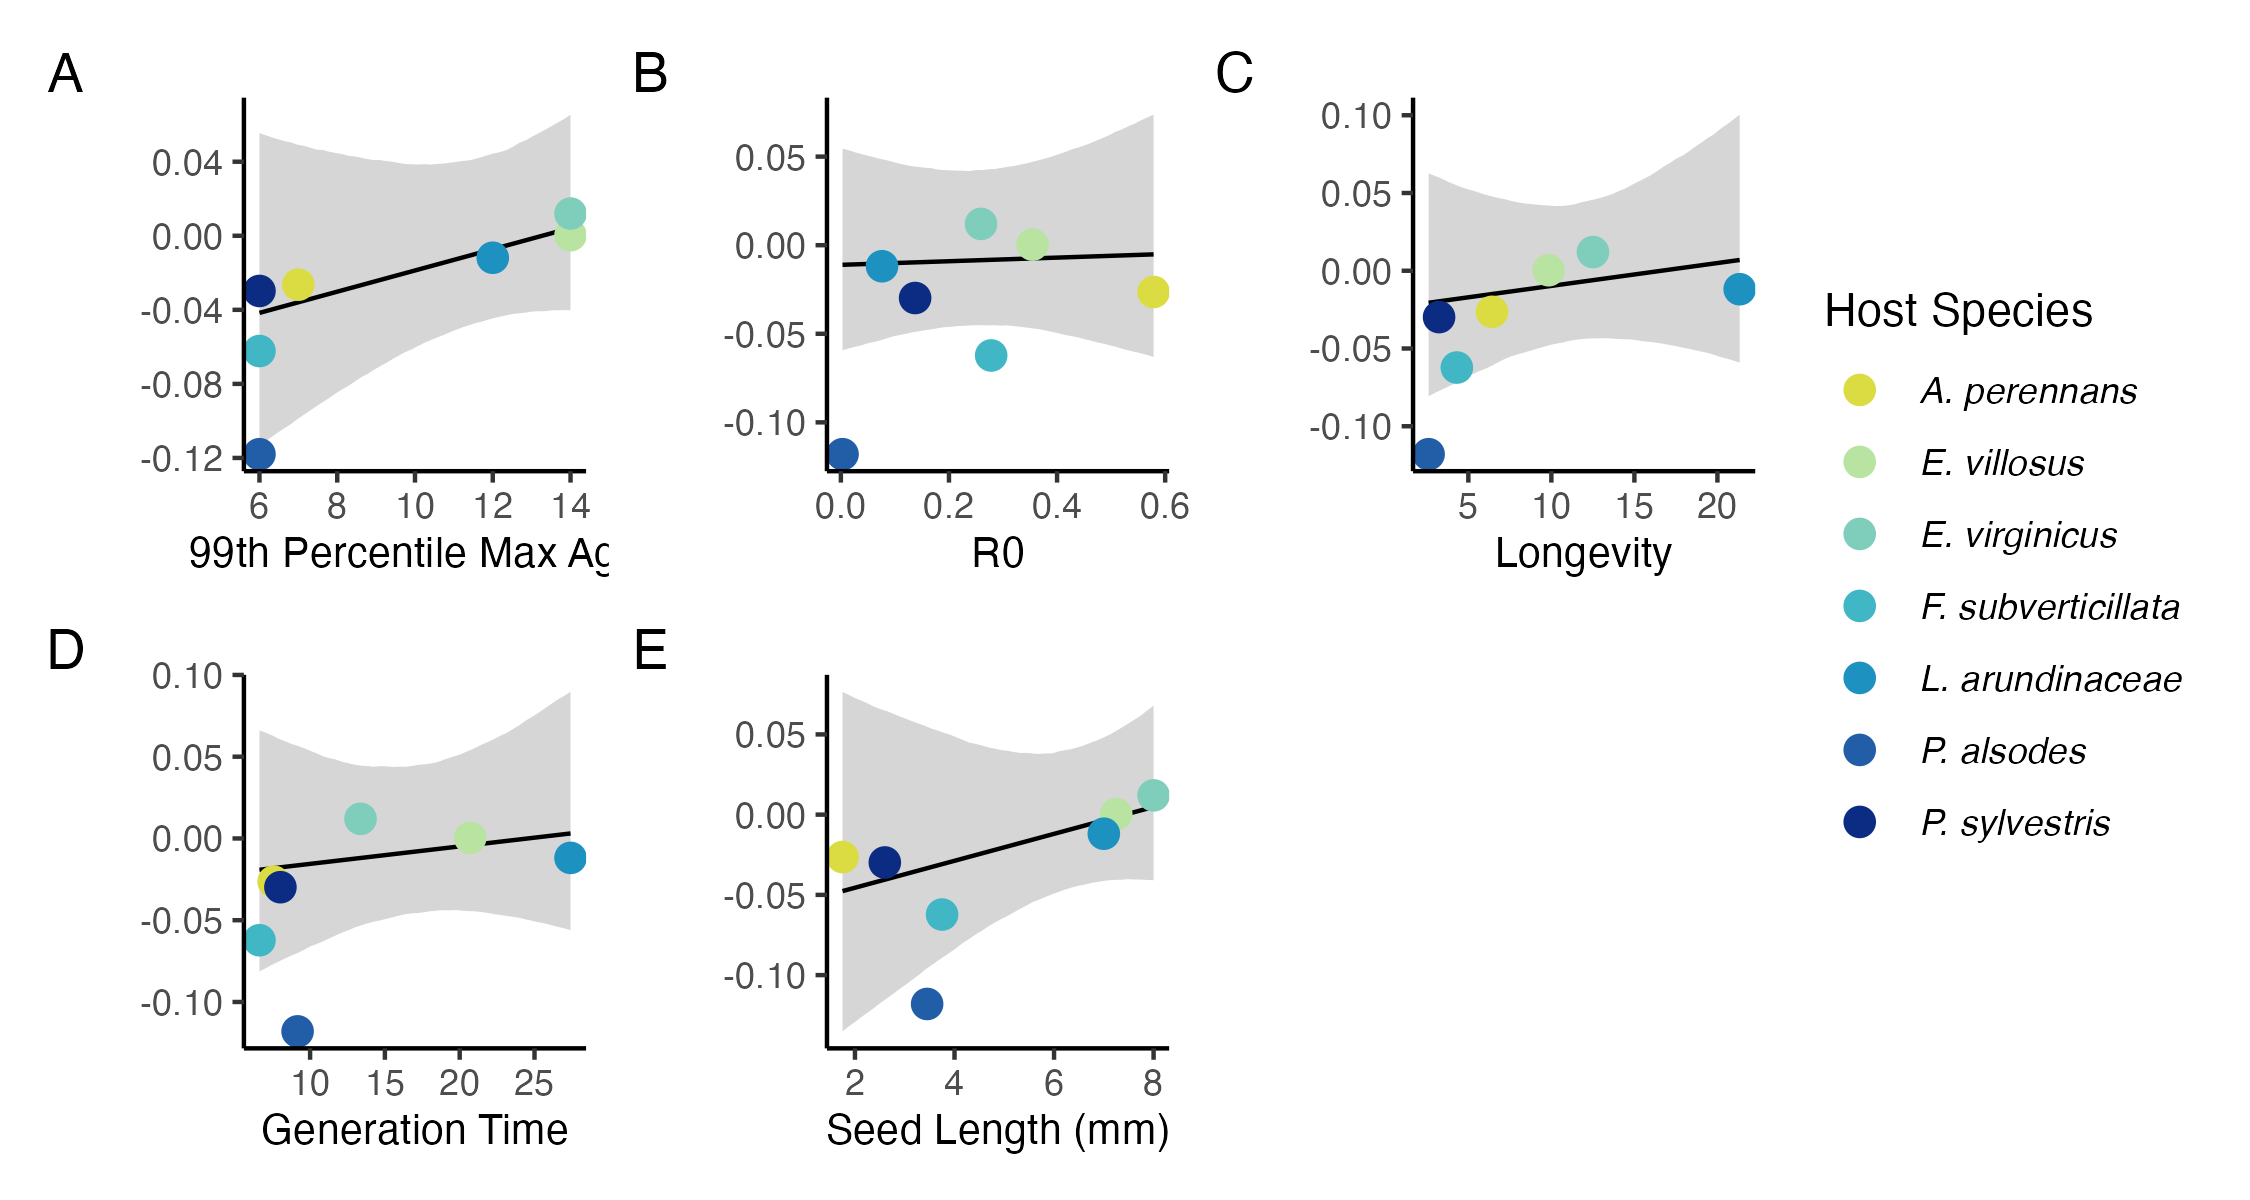
\includegraphics[width=\linewidth]{lh_epichloe_plot.png}
\end{figure}
\noindent {\bf Fig. S26.} \textbf{Relationship between variance buffering and life history traits describing the fast-slow life history continuum accounting for phylogenetic covariance between \emph{Epichlo\"{e}} symbionts.} Results are similar to regressions accounting for host plant phylogeny (Fig. 4), however symbionts are all within a single genus. Each panel shows the fitted mean relationship (line) along with with the 95\% credible interval.
\newpage


\begin{figure}
	\centering
	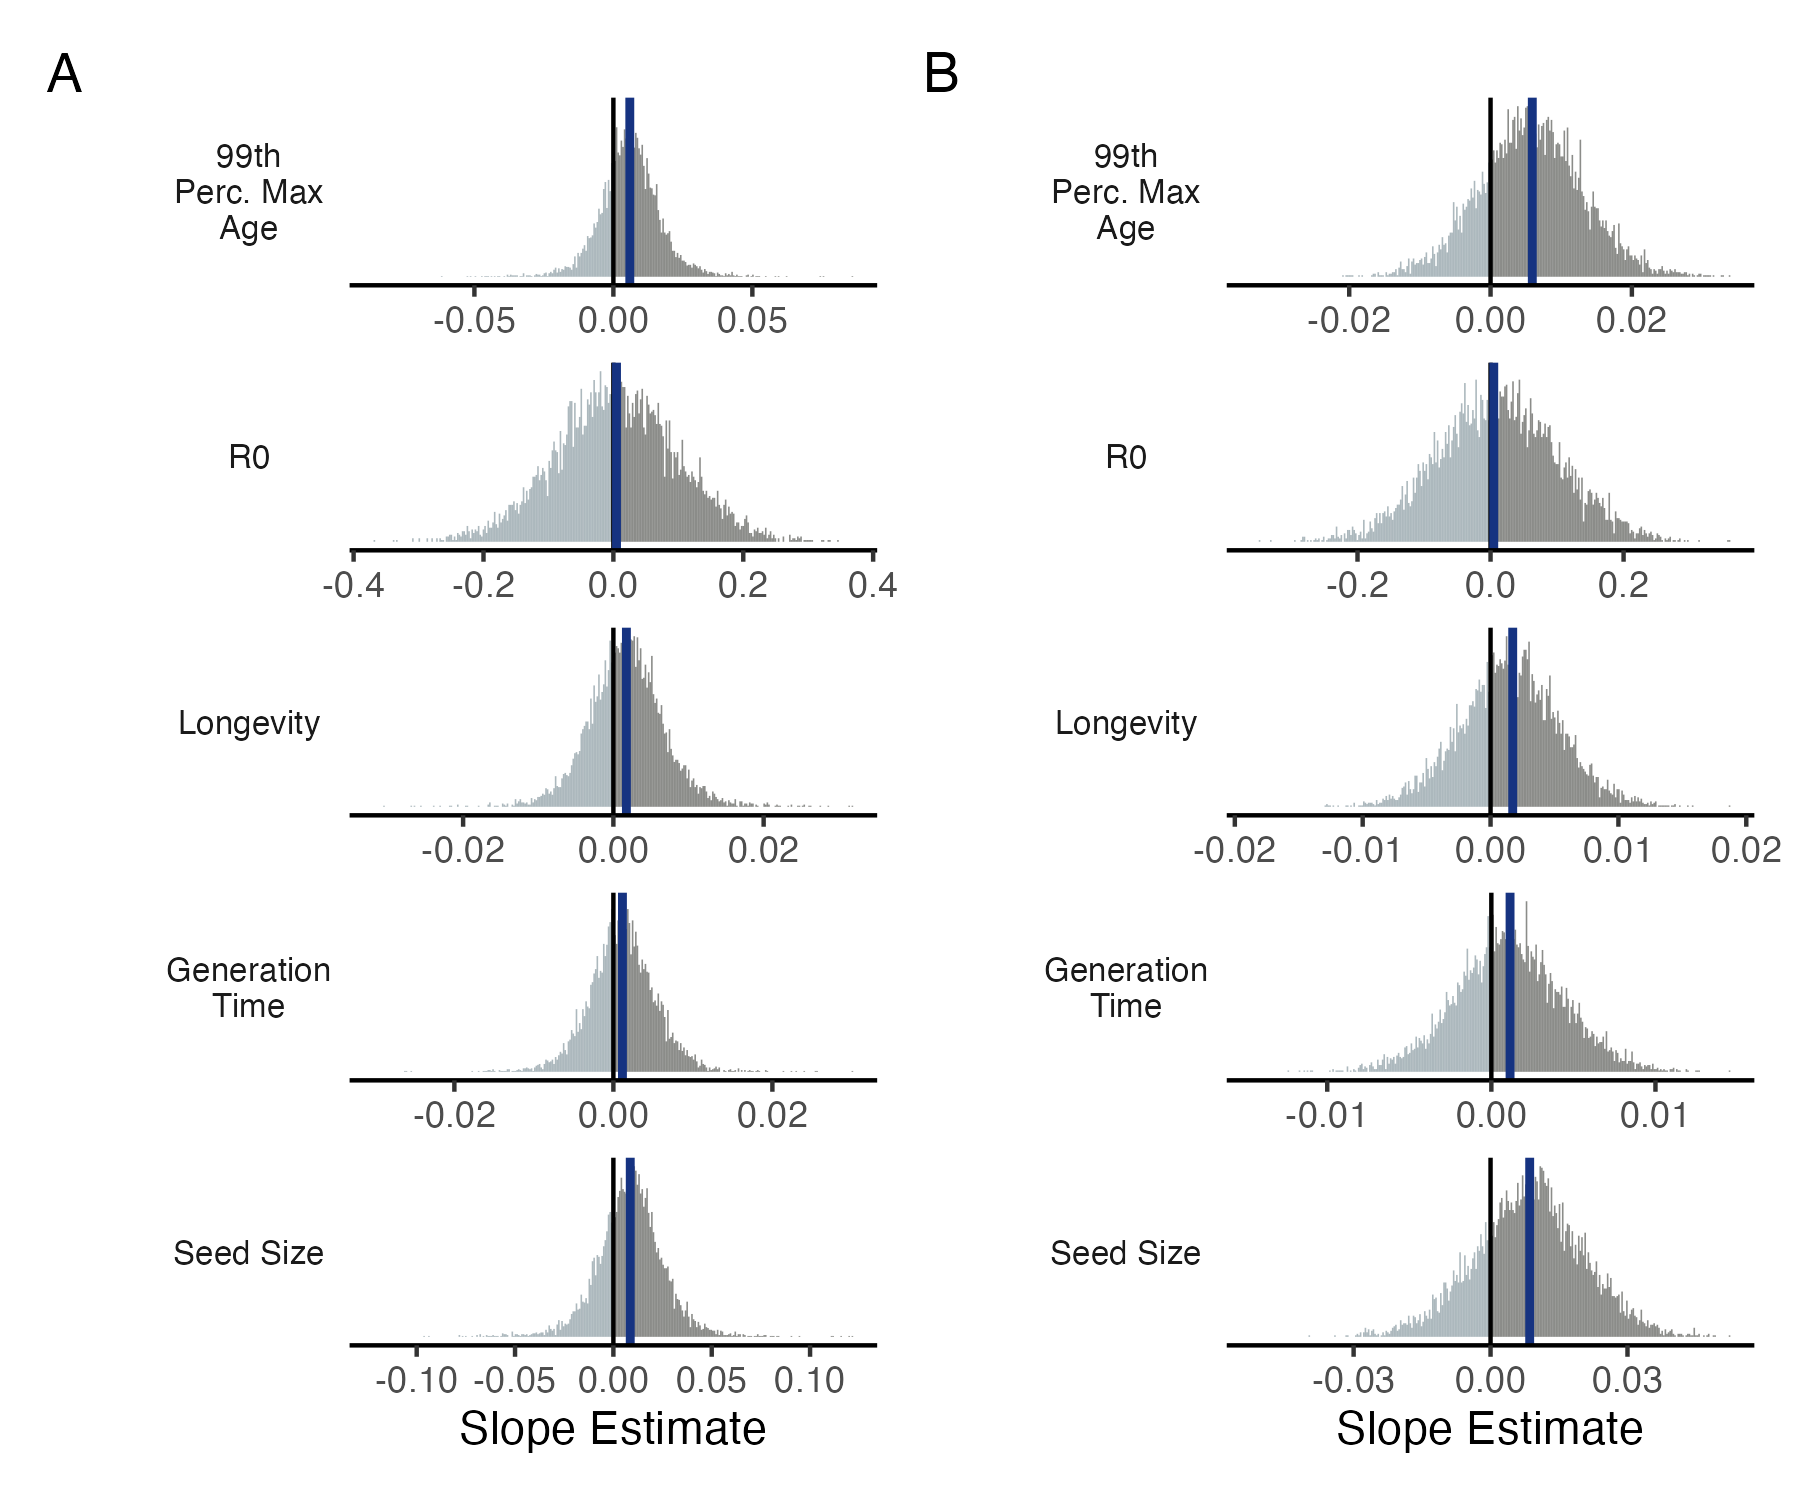
\includegraphics[width=.8\linewidth]{lh_slopes_plot.png}
\end{figure}
\noindent {\bf Fig. S27.} \textbf{Posterior estimates of life history trait effects on variance buffering.} Grey histograms show the posterior distribution of the slope parameter from models incorporating (A) host plant phylogenetic covariance and (B) symbiont phylogenetic covariance for each life history trait with blue bars showing the posterior mean.
\newpage




\noindent {\bf Table S1.} Summary of host-endophyte proprogation and transplant methods\\
\begin{table}[ht]
	\begin{adjustbox}{width=1\textwidth}
\begin{tabular}{|l|l|l|l|}
\hline
	\bf{Host Species} & \bf{Symbiont Species} & \bf{Heat treatment duration (Temp.)}& \bf{Transplant date }\\
	        \hline
	\emph{Agrostis perennans} & \emph{E. amarillans}&12 min. hot water bath (60 $^{\circ}$C)&April 2008 (10 plots)\\
	\emph{Elymus villosus} &\emph{E. elymi}&6 days drying oven (60 $^{\circ}$C)&April 2008 (10 plots)\\
	\emph{Elymus virginicus} &\emph{E. elymi or EviTG-1}&6 days drying oven (60 $^{\circ}$C)&April 2008 (10 plots)\\
	 \emph{Festuca subverticillata} &\emph{E. starrii}&6 days drying oven (60 $^{\circ}$C)&April 2008 (10 plots)\\
	 \emph{Lolium arundinaceum} &\emph{E. coenophiala}&6 days drying oven (60 $^{\circ}$C)& Sept. 2007 (10 plots)\\
	 \emph{Poa alsodes} &\emph{E. alsodes}& 7 days drying oven (60 $^{\circ}$C)&Sept. 2007 (8 plots)/April 2008 (10 plots)\\
	 \emph{Poa sylvestris}&\emph{E. PsyTG-1}&7 days drying oven (60 $^{\circ}$C)& Sept. 2007 (8 plots)/April 2008 (10 plots)\\
	 \hline
\end{tabular}
\end{adjustbox}
\end{table}


%\tom{(6d in a drying oven at 60$^{\circ}$ C for \emph{E. villosus}, \emph{E. virginicus}, \emph{F. subverticillata},  and \emph{L. arundinaceum}; 7d in a drying oven at 60$^{\circ}$ C for \emph{P. alsodes}, and \emph{P. sylvestris}; and 12 min. in a hot water bath at 60$^{\circ}$ C for \emph{A. perennans})}{need to double check methods for temp, duration, etc.}



\noindent {\bf Table S2.} Summary of focal life history traits \\
\begin{table}[ht]
\begin{adjustbox}{width=1\textwidth}{
\begin{tabular}{|p{4cm}| p{2cm} |p{2cm}|p{2cm}| p{1cm}|p{2cm}|p{2cm}|p{2.5cm}| p{2cm}|}
	\hline
	\bf{Host Species} & \bf{Observed max age}& \bf{99th perc. max age}&\bf{Generation time} & $\mathbf{R}_0$ &\bf{Longevity}&\bf{Seed Length (mm.)}&\bf{Imperfect transmission rate} & \bf{Stromata Observed}\\
	\hline
	\emph{Agrostis perennans} &11&7&7.6&0.58&6.4&1.75&69.8&No\\
	\emph{Elymus villosus}, &14&14&20.7&0.35&9.8&7.25&100&Yes\\
	\emph{Elymus virginicus} &14&14&13.4&0.25&12.5&8&100&Yes\\
	\emph{Festuca subverticillata} &9&6&6.6&0.28&4.3&3.75&42.7&No\\
	\emph{Lolium arundinaceum} &12*&12*&27.4&0.08&21.3&7&100&No\\
	\emph{Poa alsodes} &8&6&9.2&0.003&2.6&3.45&99.9&No\\
	\emph{Poa sylvestris}&12&6&8.0&0.14&3.2&2.6&16.6&Yes\\
	 \hline
\end{tabular}}
\end{adjustbox}
\end{table}

* Censuses for \emph{L. arundinaceum} plots stopped after year 12 of the experiment.


\noindent {\bf Table S3.} Summary of host-endophyte drought sensitivities\\
\begin{table}[ht]
	\begin{adjustbox}{width=1\textwidth}{
			\begin{tabular}{|p{4cm}| p{2cm} |p{2cm}|p{2cm}|p{2cm}| p{2cm}|p{2cm}|p{2cm}|p{2cm}|}
				\hline
				\bf{Host Species} & \bf{Effect on CV($\lambda$)}& \bf{Effect on Mean($\lambda$)}&$\frac{\Delta\lambda^{-}}{\Delta SPEI_{3}}$ & $\frac{\Delta\lambda^{+}}{\Delta SPEI_{3}}$ &\bf{3 month S- to S+ ratio}&$\frac{\Delta\lambda^{-}}{\Delta SPEI_{12}}$ &$\frac{\Delta\lambda^{+}}{\Delta SPEI_{12}}$ &\bf{12 month S- to S+ ratio}\\
				\hline
				\emph{Agrostis perennans} &-0.02641&0.04412&0.0341&-0.0400&0.85&0.11410&-0.06255&1.82\\
				\emph{Elymus villosus}, &0.00033&0.05089&-0.0267&0.0137&1.95&0.02968&0.04216&0.70\\
				\emph{Elymus virginicus} &0.01201&0.05775&0.0697&0.0465&1.50&0.09677&0.06803&1.42\\
				\emph{Festuca subverticillata} &-0.06225&0.16393&0.0213&0.0212&1.01&-0.12873&-0.09010&1.43\\
				\emph{Lolium arundinaceum} &-0.01188&0.10215&-0.0119&0.0090&1.32&0.02644&-0.02596&1.02\\
				\emph{Poa alsodes} &-0.11798&0.12816&0.1017&0.1429&0.71&0.10457&0.14328&0.73\\
				\emph{Poa sylvestris}&-0.02981&-0.00852&0.0717&0.1600&0.44&0.05445&0.09820&0.55\\
				\hline
		\end{tabular}}
	\end{adjustbox}
\end{table}



\end{document}





















